\documentclass[]{book}
\usepackage{lmodern}
\usepackage{amssymb,amsmath}
\usepackage{ifxetex,ifluatex}
\usepackage{fixltx2e} % provides \textsubscript
\ifnum 0\ifxetex 1\fi\ifluatex 1\fi=0 % if pdftex
  \usepackage[T1]{fontenc}
  \usepackage[utf8]{inputenc}
\else % if luatex or xelatex
  \ifxetex
    \usepackage{mathspec}
  \else
    \usepackage{fontspec}
  \fi
  \defaultfontfeatures{Ligatures=TeX,Scale=MatchLowercase}
\fi
% use upquote if available, for straight quotes in verbatim environments
\IfFileExists{upquote.sty}{\usepackage{upquote}}{}
% use microtype if available
\IfFileExists{microtype.sty}{%
\usepackage{microtype}
\UseMicrotypeSet[protrusion]{basicmath} % disable protrusion for tt fonts
}{}
\usepackage[margin=1in]{geometry}
\usepackage{hyperref}
\hypersetup{unicode=true,
            pdftitle={Applied Missing data analysis with SPSS and R(Studio)},
            pdfauthor={Martijn Heymans and Iris Eekhout},
            pdfborder={0 0 0},
            breaklinks=true}
\urlstyle{same}  % don't use monospace font for urls
\usepackage{natbib}
\bibliographystyle{apalike}
\usepackage{color}
\usepackage{fancyvrb}
\newcommand{\VerbBar}{|}
\newcommand{\VERB}{\Verb[commandchars=\\\{\}]}
\DefineVerbatimEnvironment{Highlighting}{Verbatim}{commandchars=\\\{\}}
% Add ',fontsize=\small' for more characters per line
\usepackage{framed}
\definecolor{shadecolor}{RGB}{248,248,248}
\newenvironment{Shaded}{\begin{snugshade}}{\end{snugshade}}
\newcommand{\KeywordTok}[1]{\textcolor[rgb]{0.13,0.29,0.53}{\textbf{#1}}}
\newcommand{\DataTypeTok}[1]{\textcolor[rgb]{0.13,0.29,0.53}{#1}}
\newcommand{\DecValTok}[1]{\textcolor[rgb]{0.00,0.00,0.81}{#1}}
\newcommand{\BaseNTok}[1]{\textcolor[rgb]{0.00,0.00,0.81}{#1}}
\newcommand{\FloatTok}[1]{\textcolor[rgb]{0.00,0.00,0.81}{#1}}
\newcommand{\ConstantTok}[1]{\textcolor[rgb]{0.00,0.00,0.00}{#1}}
\newcommand{\CharTok}[1]{\textcolor[rgb]{0.31,0.60,0.02}{#1}}
\newcommand{\SpecialCharTok}[1]{\textcolor[rgb]{0.00,0.00,0.00}{#1}}
\newcommand{\StringTok}[1]{\textcolor[rgb]{0.31,0.60,0.02}{#1}}
\newcommand{\VerbatimStringTok}[1]{\textcolor[rgb]{0.31,0.60,0.02}{#1}}
\newcommand{\SpecialStringTok}[1]{\textcolor[rgb]{0.31,0.60,0.02}{#1}}
\newcommand{\ImportTok}[1]{#1}
\newcommand{\CommentTok}[1]{\textcolor[rgb]{0.56,0.35,0.01}{\textit{#1}}}
\newcommand{\DocumentationTok}[1]{\textcolor[rgb]{0.56,0.35,0.01}{\textbf{\textit{#1}}}}
\newcommand{\AnnotationTok}[1]{\textcolor[rgb]{0.56,0.35,0.01}{\textbf{\textit{#1}}}}
\newcommand{\CommentVarTok}[1]{\textcolor[rgb]{0.56,0.35,0.01}{\textbf{\textit{#1}}}}
\newcommand{\OtherTok}[1]{\textcolor[rgb]{0.56,0.35,0.01}{#1}}
\newcommand{\FunctionTok}[1]{\textcolor[rgb]{0.00,0.00,0.00}{#1}}
\newcommand{\VariableTok}[1]{\textcolor[rgb]{0.00,0.00,0.00}{#1}}
\newcommand{\ControlFlowTok}[1]{\textcolor[rgb]{0.13,0.29,0.53}{\textbf{#1}}}
\newcommand{\OperatorTok}[1]{\textcolor[rgb]{0.81,0.36,0.00}{\textbf{#1}}}
\newcommand{\BuiltInTok}[1]{#1}
\newcommand{\ExtensionTok}[1]{#1}
\newcommand{\PreprocessorTok}[1]{\textcolor[rgb]{0.56,0.35,0.01}{\textit{#1}}}
\newcommand{\AttributeTok}[1]{\textcolor[rgb]{0.77,0.63,0.00}{#1}}
\newcommand{\RegionMarkerTok}[1]{#1}
\newcommand{\InformationTok}[1]{\textcolor[rgb]{0.56,0.35,0.01}{\textbf{\textit{#1}}}}
\newcommand{\WarningTok}[1]{\textcolor[rgb]{0.56,0.35,0.01}{\textbf{\textit{#1}}}}
\newcommand{\AlertTok}[1]{\textcolor[rgb]{0.94,0.16,0.16}{#1}}
\newcommand{\ErrorTok}[1]{\textcolor[rgb]{0.64,0.00,0.00}{\textbf{#1}}}
\newcommand{\NormalTok}[1]{#1}
\usepackage{longtable,booktabs}
\usepackage{graphicx,grffile}
\makeatletter
\def\maxwidth{\ifdim\Gin@nat@width>\linewidth\linewidth\else\Gin@nat@width\fi}
\def\maxheight{\ifdim\Gin@nat@height>\textheight\textheight\else\Gin@nat@height\fi}
\makeatother
% Scale images if necessary, so that they will not overflow the page
% margins by default, and it is still possible to overwrite the defaults
% using explicit options in \includegraphics[width, height, ...]{}
\setkeys{Gin}{width=\maxwidth,height=\maxheight,keepaspectratio}
\IfFileExists{parskip.sty}{%
\usepackage{parskip}
}{% else
\setlength{\parindent}{0pt}
\setlength{\parskip}{6pt plus 2pt minus 1pt}
}
\setlength{\emergencystretch}{3em}  % prevent overfull lines
\providecommand{\tightlist}{%
  \setlength{\itemsep}{0pt}\setlength{\parskip}{0pt}}
\setcounter{secnumdepth}{5}
% Redefines (sub)paragraphs to behave more like sections
\ifx\paragraph\undefined\else
\let\oldparagraph\paragraph
\renewcommand{\paragraph}[1]{\oldparagraph{#1}\mbox{}}
\fi
\ifx\subparagraph\undefined\else
\let\oldsubparagraph\subparagraph
\renewcommand{\subparagraph}[1]{\oldsubparagraph{#1}\mbox{}}
\fi

%%% Use protect on footnotes to avoid problems with footnotes in titles
\let\rmarkdownfootnote\footnote%
\def\footnote{\protect\rmarkdownfootnote}

%%% Change title format to be more compact
\usepackage{titling}

% Create subtitle command for use in maketitle
\newcommand{\subtitle}[1]{
  \posttitle{
    \begin{center}\large#1\end{center}
    }
}

\setlength{\droptitle}{-2em}

  \title{Applied Missing data analysis with SPSS and R(Studio)}
    \pretitle{\vspace{\droptitle}\centering\huge}
  \posttitle{\par}
    \author{Martijn Heymans and Iris Eekhout}
    \preauthor{\centering\large\emph}
  \postauthor{\par}
      \predate{\centering\large\emph}
  \postdate{\par}
    \date{2018-09-19}

\usepackage{booktabs}

\begin{document}
\maketitle

{
\setcounter{tocdepth}{1}
\tableofcontents
}
\chapter*{Preface}\label{preface}
\addcontentsline{toc}{chapter}{Preface}

The attention for missing data is growing and so will be the application
of methods to solve the missing data problem. From our experience,
researchers with missing data still find it difficult to reserve time to
evaluate the missing data and from that to find a reasonable solution to
handle their missing data for their main data analysis. This manual is
developed for researchers that are looking for a solution of their
missing data problem or want to learn more about missing data. The
manual is developed as a result of a missing data course that we give.
Further, we are also active in providing statistical advice in general
and more specific about missing data. Because our time to give advice is
mostly limited we wanted to give researchers a practical guide to help
them get started with their missing data problem. Leading methodologists
and statisticians and leading journals have published papers about the
problems of missing data and warned researchers to take missing data
seriously (Sterne et al., BMJ 2009, Little et al. NEJM 2012, Peng et al.
2015, JAMA). Hopefully this manual will help researchers to find the
best solution for their missing data problem. We hope you will enjoy
this manual and that you learn from it, at least to take missing data
seriously and that you will use recommended methods to solve your
missing data problem.

\section{The goal of this Manual}\label{the-goal-of-this-manual}

In this manual the software packages SPSS and R play a central role. The
combination of these two software packages may seem a coincidence, but
it is not. For a long time, SPSS was the most popular software package
worldwide to do statistical data analysis. Currently, R is growing in
popularity fast and will probably become one of the most popular
Software packages to do data analysis. Also for applied researchers.
Both SPSS and R have their advantages and disadvantages. An advantage of
SPSS is that it is a user-friendly software package compared to R and
works with windows where you can for example drag your variables to.
Subsequently, you can click the OK button and the statistical analysis
procedure you prespecified gives you the output results. A disadvantage
of SPSS may be that you are overloaded with statistical output that may
not all needed to answer your research question. Compared to SPSS you
could say that R is a more user-unfriendly software package where you
need to use R code to activate statistical procedures and to get
statistical results. R output will show more specific results, without
extra information. Furthermore, R works much faster when it comes to
running statistical procedures by using 1 or 2 lines of R code, compared
to visiting a couple of windows in SPSS to activate the same statistical
test. There is one other advantage of R and that is, that it is open
source. This makes it possible for applied researchers to follow the
calculations of complex procedures as the estimation of missing values
closely along the line. You could say that R brings you to the heart of
the matter. With R it is possible to turn complex data analysis
functions and formula´s into computer code that can be used by everybody
and vice versa. Because it is open source, you are able to read the code
that is used for the analysis and to relate that code or pieces of code
to the statistical output. This makes it possible to evaluate step by
step the code and thus the statistical procedures and relate them to the
subsequent results. You can copy specific parts of code from functions
that others have written and evaluate what happens. This is one of the
major advantages of R if you compare it to the closed source statistical
package SPSS. R brings you a big learning environment when it comes to
the understanding of all kind of statistical procedures as missing data
analysis.

\section{Multiple Imputation in SPSS and
R}\label{multiple-imputation-in-spss-and-r}

Multiple Imputation (MI) is a procedure that is developed in the 1970's
by Donald Rubin. Later, around the 1990´s Multiple imputation was
further developed and became more popular. For a long time, MI was only
available for S-Plus and R software (S-plus is the commercial
alternative of R), where it was further developed by Stef van Buuren, a
statistician from TNO, Leiden, The Netherlands. For a long time, it was
not possible to do MI analysis in SPSS because it was not available in
SPSS. So, it was far out of reach for applied researchers for a long
time. It became available from SPSS version 17. From that time MI is now
used more by applied researchers. In this manual the handling of missing
data is the main topic. We will also show how to apply these methods in
both software packages SPSS and R. To apply the imputation methods that
are discussed both software packages make use of random starting
procedures. SPSS and R use for that intern random number generators.
Because these are different, result might slightly differ. Our intention
is not to compare the software packages SPSS and R and their output
resultys. Both are trustful packages, it is more the estimation
procedures that might lead to the differences. The imputation methods,
will be applied in SPSS version 24 and with R software version 3.4.3.
The R examples will be presented by using the output from RStudio
version (version 1.1.383 -- © 2009-2017 RStudio, Inc.). RStudio is an
integrated development environment (IDE) for R. RStudio includes a wide
range of productivity enhancing features and runs on all major
platforms. As already stated, R allows you to program the statistical
formula's yourself. We have therefore chosen to explain the formula's in
more detail in combination with the application in R. The more applied
researchers will be satisfied with the explanation and application of
methods in SPSS.

\section{Notation and annotation in this
manual}\label{notation-and-annotation-in-this-manual}

The name of R packages, libraries and functions can be recognized by
using Courier new lettertype, for example the package mice will be
written as mice.

R code of the procedures used in the manual is marked grey and the
explanation in these grey parts can be found in the grey parts itself
annotated by the \# symbol. The lines that start with the symbol
\textgreater{} are R Code lines that have been running in the R Console
in RStudio. Example:

\textbf{R code XX}

\begin{Shaded}
\begin{Highlighting}[]
\CommentTok{# Activate the foreign package and read in the SPSS dataset}

\KeywordTok{library}\NormalTok{(foreign)}
\NormalTok{dataset <-}\StringTok{ }\KeywordTok{read.spss}\NormalTok{(}\DataTypeTok{file=}\StringTok{"data/Backpain 50 missing.sav"}\NormalTok{, }\DataTypeTok{to.data.frame=}\NormalTok{T)}
\end{Highlighting}
\end{Shaded}

\begin{verbatim}
## re-encoding from UTF-8
\end{verbatim}

\chapter{Software applications}\label{software-applications}

Statistical software programs can help us to analyze our data. SPSS and
R are such programs. Although SPSS and R are among the most popular
programs to do statistical data analyses nowadays, they do not have much
in common. One of the greatest differences is that SPSS works with menu
options that make windows appear and you can click buttons to select
options, whereas R works with lines of code that you have to type in to
run analyses. This makes SPSS more user-friendly than R for applied
researchers. In SPSS you are overloaded with output tables, and in R you
only get output on demand. In this Chapter we will explore the different
possibilities of the SPSS (IBM 2016) and the R software language
(Matloff, 2011, Dalgaard, 2008). We will run R via RStudio, the
integrated development environment (IDE) for R. RStudio includes a wide
range of productivity enhancing features, which makes it easier to work
with than with the R console on its own.

\section{SPSS, Data and Variable View
windows}\label{spss-data-and-variable-view-windows}

In this manual we work with SPSS version 24 (IBM, 2016). When you start
SPSS Version 24 a start-up window appears. In this window, you can
directly open the files that were active during your previous use of
SPSS. These files can be found and easily opened in the ``Recent files''
window (Figure \ref{fig:fig1}). If you do not want to see this window
the next time that you open SPSS, select ``Don't show this dialog in the
future''.

\begin{figure}

{\centering 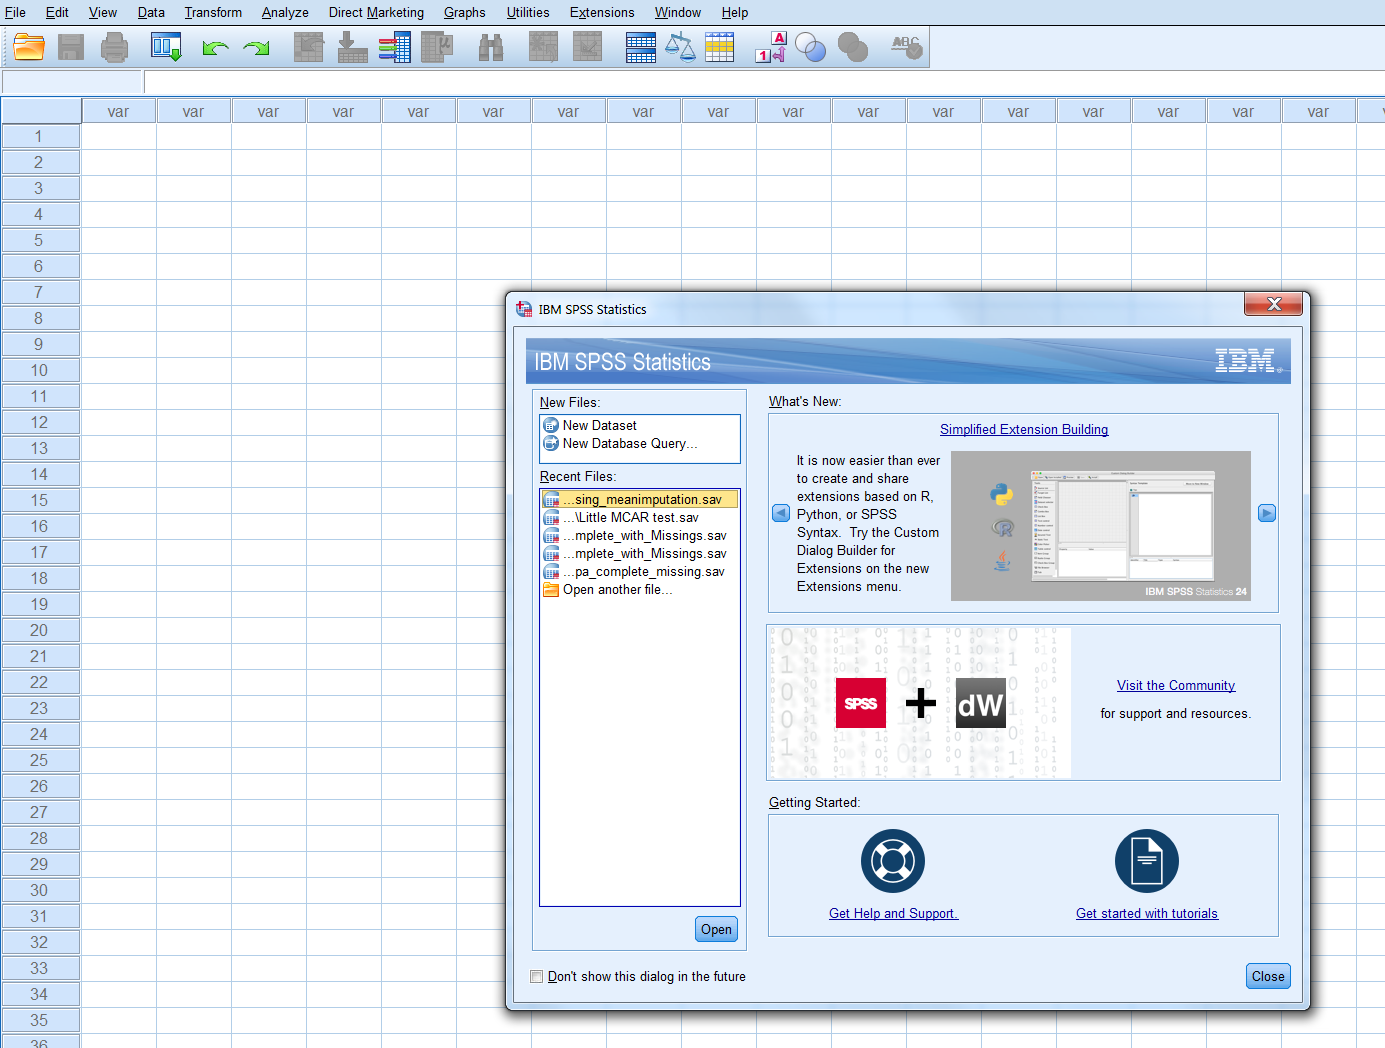
\includegraphics[width=0.9\linewidth]{images/fig1.1} 

}

\caption{First window after you have started SPSS}\label{fig:fig1}
\end{figure}

When you click on Close on the right side below, the window will close
and you will see an empty Data View window. Now you are in the SPSS Data
Editor window. This window is always open when you start SPSS. The name
``SPSS Data Editor'' is also visible at the top of the screen and is
called ``IBM SPSS Statistics Data Editor'' (Figure \ref{fig:fig2}).

\begin{figure}

{\centering 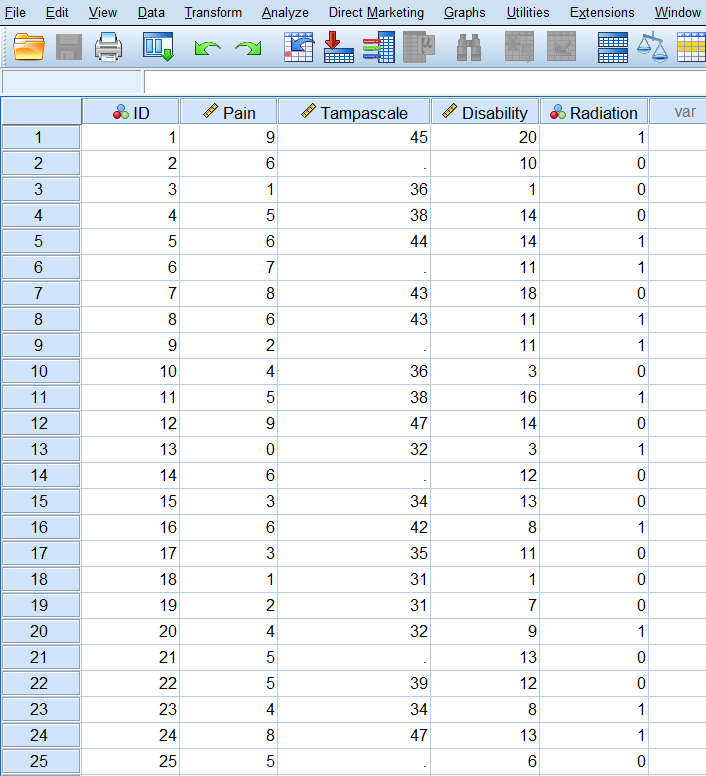
\includegraphics[width=0.9\linewidth]{images/fig1.2} 

}

\caption{Data View window in SPSS}\label{fig:fig2}
\end{figure}

In the SPSS Data Editor, you have the possibility to go to the Data View
and Variable View windows. In the Data View window, you can enter data
yourself or read in data by using the options in the file menu. In
Figure 1.2 you see an example of a dataset in the Data View window. Each
row in the Data View window represents a case and in the columns you
will find the variable names. In the Data View window, you can do all
kind of data manipulations by using the different menu's above in the
window. From here you can click on the tab Variable View, in the lower
left corner of the window. Than the Variable view window will appear
(Figure \ref{fig:fig3}).

\begin{figure}

{\centering 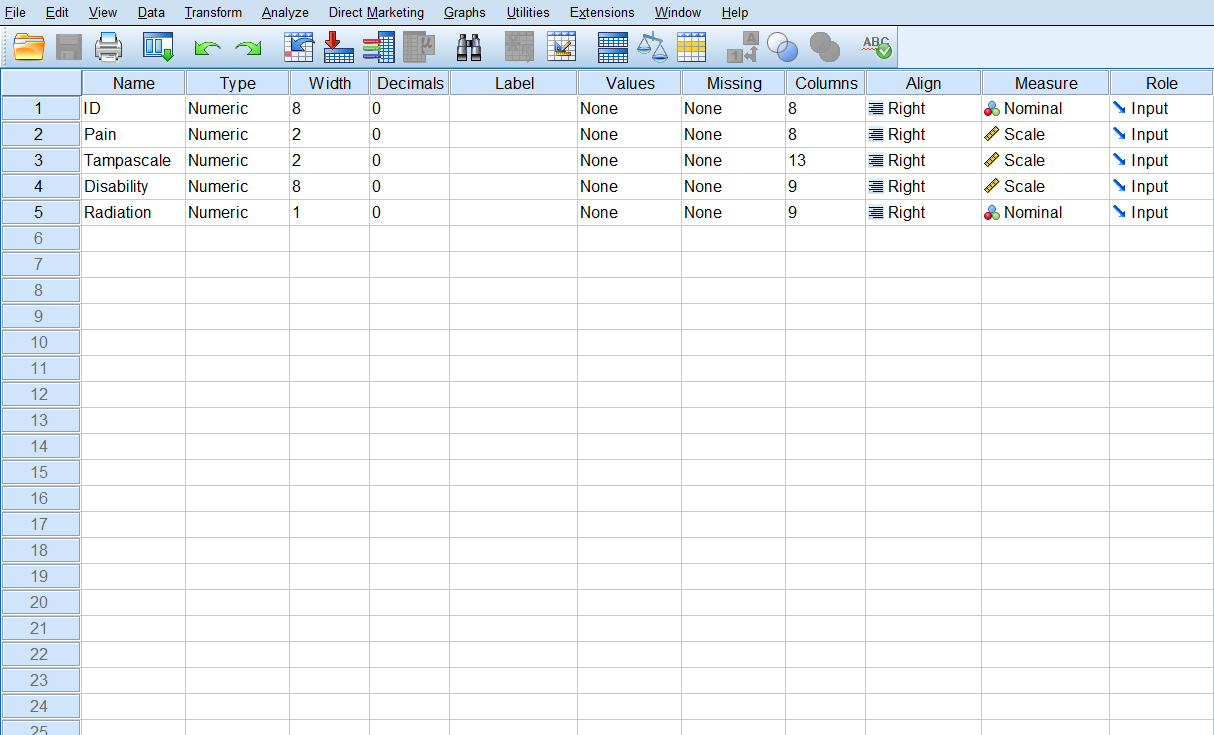
\includegraphics[width=0.9\linewidth]{images/fig1.3} 

}

\caption{Variable View window in SPSS}\label{fig:fig3}
\end{figure}

In the Variable View window, you can add new variables, by entering the
name in the name column. Further, you can change the columns by using
the following options: Type: Here you can change the type of variables
in your dataset. Mostly you work with numeric variables, i.e.~a variable
whose values are numbers. Other possibilities are Date variables which
is a numeric variable whose values are displayed in one of several
calendar-date or clock-time formats or String variables, a character
(text) variable that can contain any characters up to the defined
length. String values are not numeric and therefore are not used in
calculations. Width: By default SPSS defines a numeric variable with 8
digits for each new variable.

Decimals: the number of decimal places displayed.

Label: The variable name.

Values: To assign numbers to the categories of a variable. To define
Variable values do the following: 1. Click the button in the Values cell
for the variable that you want to define. 2. For each value, enter the
value and a label. 3. Click Add to enter the value label. 4. Click OK.

Missing: Here you can define specified data values as user-missing. You
can enter up to three discrete (individual) missing values, a range of
missing values, or a range plus one discrete value.

Columns: To change the number of characters displayed in the Data View
window.

Align: Here you can specify the alignment of your data.

Measure: Here you can specify the level of each variable, scale
(continuous), ordinal or nominal.

Role: Here you can define the role of the variable during your analysis.
Examples are, Input for independent variable, Target for dependent or
outcome variable, Both, independent and dependent variable. There are
more possibilities, but most of the times you use the default Input
setting.

\section{Analyzing data in SPSS}\label{analyzing-data-in-spss}

All statistical procedures in SPSS can be found under the Analyze button
(Figure \ref{fig:fig4}). Here you also will find the option ``Multiple
Imputation'' which plays an important role in this manual. We will use
this menu later on in Chapter 4.

\begin{figure}

{\centering 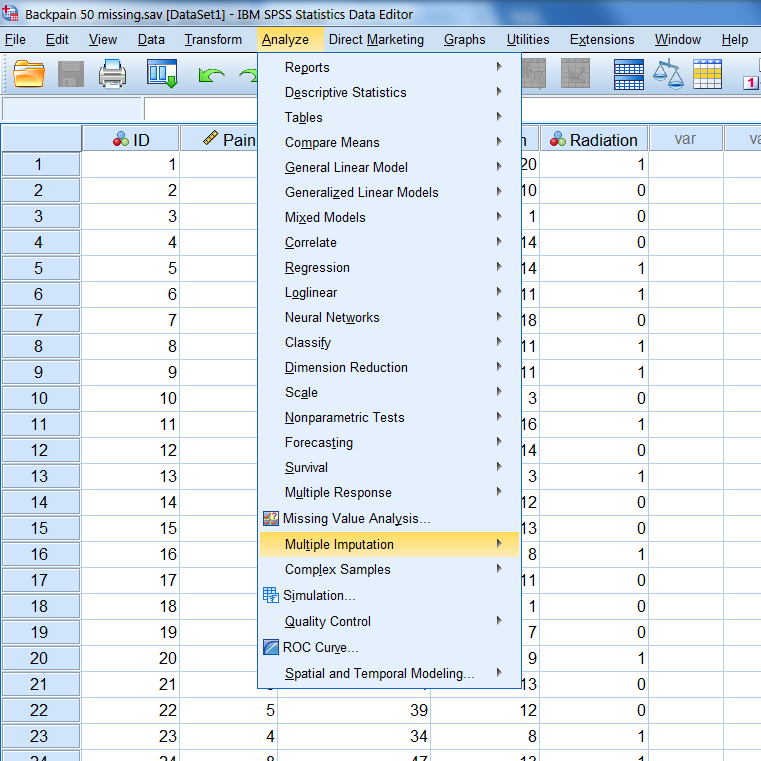
\includegraphics[width=0.9\linewidth]{images/fig1.4} 

}

\caption{Statistical procedures that can be found under the Analyze menu in SPSS}\label{fig:fig4}
\end{figure}

\section{Data Transformations in
SPSS}\label{data-transformations-in-spss}

Two other interesting buttons are Data and Transform. The Data menu
allows you to make changes to the data editor. Here you can add new
variables or cases. You can also use the Split File option, to get
analyses results separately for categories of a variable. The Transform
menu allows you to manipulate your variables by for example
dichotomizing a numeric variable.

\section{The Output window in SPSS}\label{the-output-window-in-spss}

If you have run your analyses in SPSS, an SPSS Output (or viewer) Window
will pop-up. The main body of the Output Window consists of two panes
(left and right panes). In the left pane you will find an outline of the
output. In the right pane you will find the actual output of your
statistical procedure (Figure \ref{fig:fig5}).

\begin{figure}

{\centering 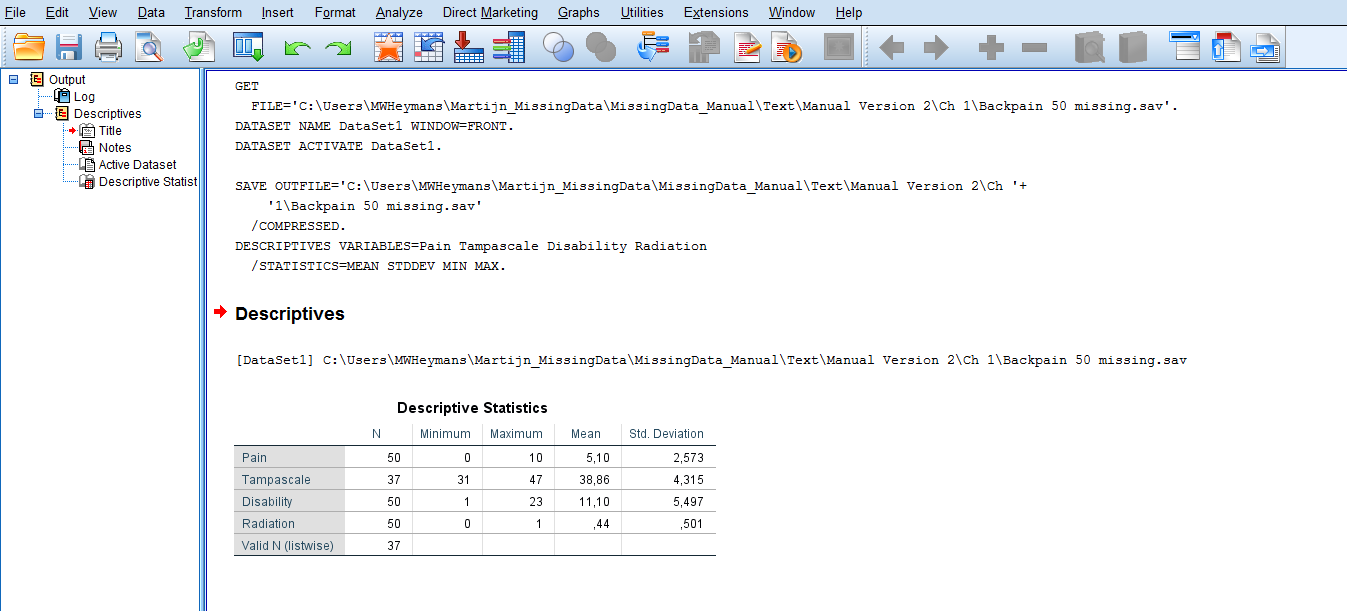
\includegraphics[width=0.9\linewidth]{images/fig1.5} 

}

\caption{Part of the Output or Viewer window in SPSS after making use of Descriptive Statistics under the Analyze menu}\label{fig:fig5}
\end{figure}

\section{The Syntax Editor in SPSS}\label{the-syntax-editor-in-spss}

In the syntax editor of SPSS, you use the SPSS syntax programming
language. You can run all SPSS procedures by typing in commands in this
syntax editor window, instead of using the graphical user interface,
i.e.~by using your mouse and clicking on the menu´s. You can get access
to the syntax window in two ways. The first is just by opening a new
syntax file by navigating to File -\textgreater{} New -\textgreater{}
Syntax. This will open a new syntax window (Figure \ref{fig:fig6}).

\begin{figure}

{\centering 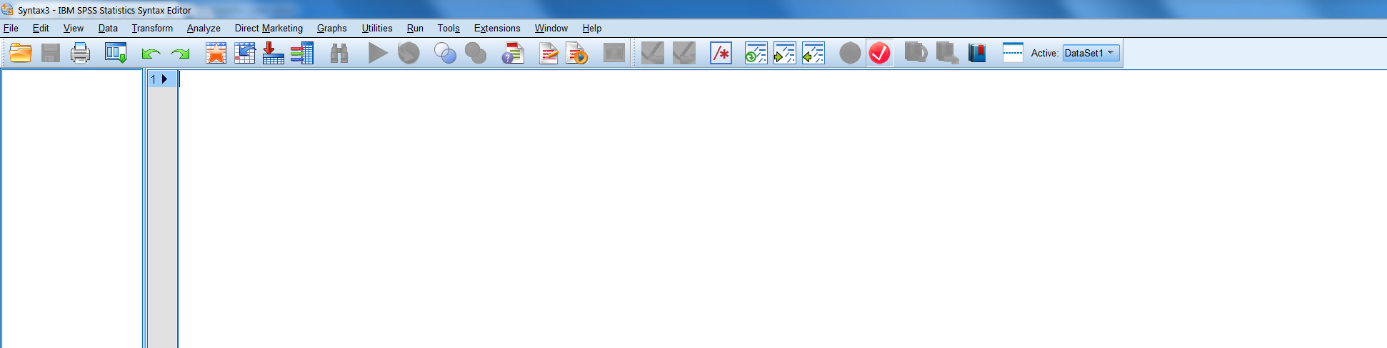
\includegraphics[width=0.9\linewidth]{images/fig1.6} 

}

\caption{Screenshot of new syntax file}\label{fig:fig6}
\end{figure}

Now you can start writing your syntax directly in this window. You can
also generate syntax by accessing statistical procedures through the
dropdown menus and clicking the Paste button instead of clicking the OK
button after you have specified the options. When you have clicked the
Paste button, a new Syntax Editor window will pop up or the new syntax
will automatically be added to the open Syntax Editor window. This is a
very useful way to keep track of the analysis that you have performed.
An example can be found in Figure \ref{fig:fig7}, where the syntax is
shown for the Descriptive Statistics procedure of Figure \ref{fig:fig5}.

\begin{figure}

{\centering 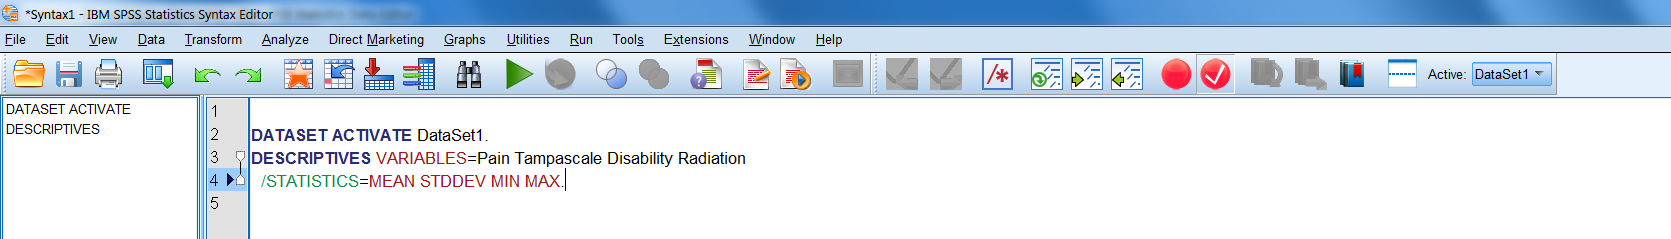
\includegraphics[width=0.9\linewidth]{images/fig1.7} 

}

\caption{Screenshot of Syntax editor of SPSS including the Syntax code for descriptive statisitcs}\label{fig:fig7}
\end{figure}

By using the SPSS Syntax it is possible for users to perform the same
analyses over and over again or to adapt the analysis via the syntax
code for complex calculations in the data. In this manual we will not
use SPSS syntax code to access statistical procedures, however we
recommend to use the SPSS syntax to keep track of the analysis that you
have performed. SPSS is most frequently used via the graphical user
interface, and we will use that method also in this manual.

\section{Reading and saving data in
SPSS}\label{reading-and-saving-data-in-spss}

Reading in data in SPSS is very easy; via the menu File choose for File
-\textgreater{} Open -\textgreater{} Data. All kind of file types can be
selected. Of course the SPSS .sav files, but also .por, .xlsx, .cvs,
SAS, Stata, etc. (Figure 1.8). After you have selected a specific file
type you may have to go through several steps before you see the data in
the Data View window. These steps are not necessary for SPSS files, they
open directly in the data editor.

\begin{figure}

{\centering 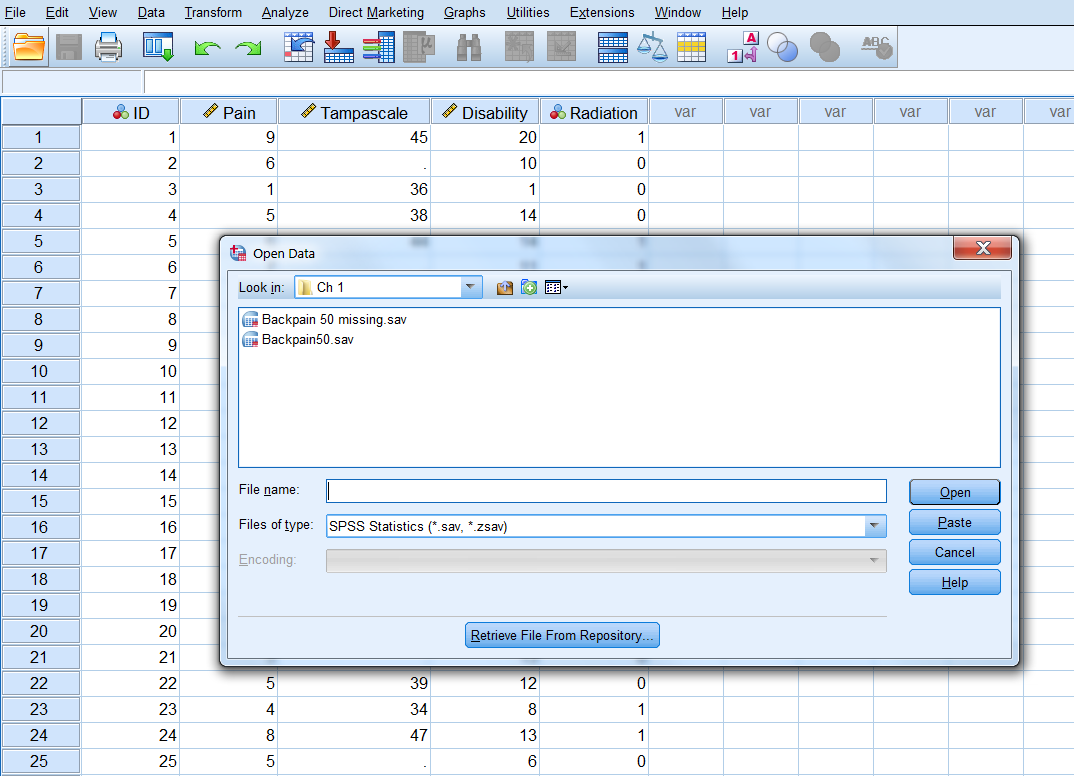
\includegraphics[width=0.9\linewidth]{images/fig1.8} 

}

\caption{Window to read in different file types in SPSS}\label{fig:fig8}
\end{figure}

Saving files in SPSS is possible via the Save Data As option under the
menu File. You can choose the same kind of file types (Figure
\ref{fig:fig9}).

\begin{figure}

{\centering 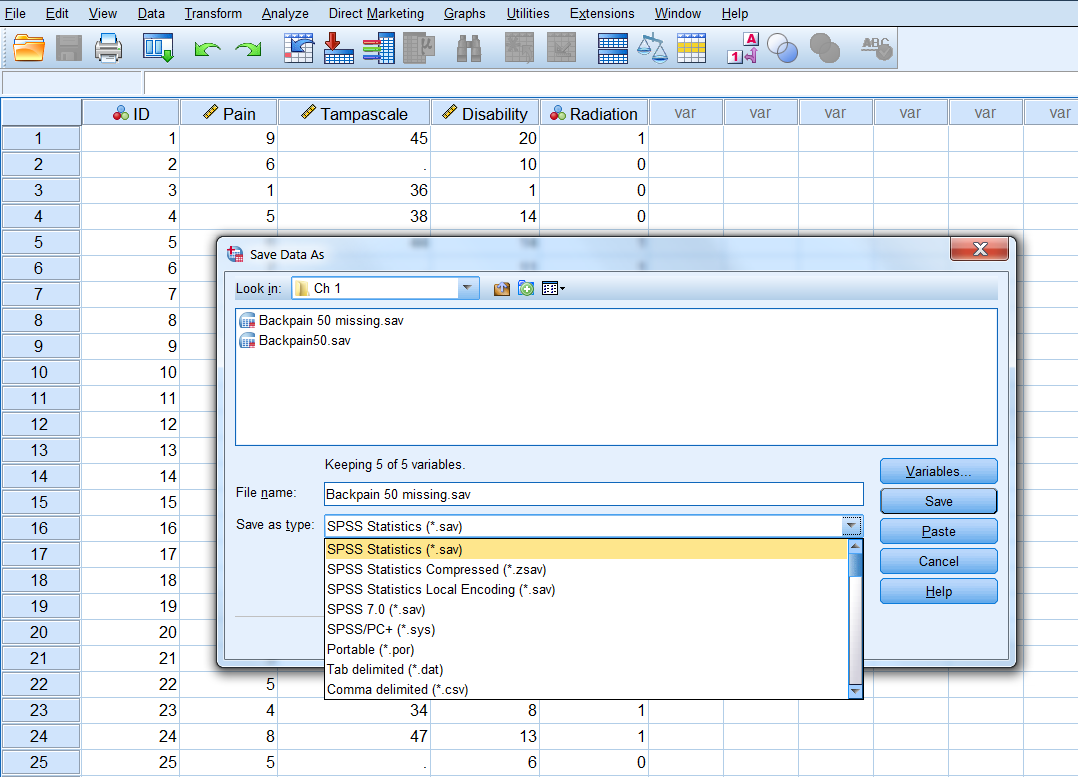
\includegraphics[width=0.9\linewidth]{images/fig1.9} 

}

\caption{Option Save Data As under the menu File}\label{fig:fig9}
\end{figure}

\section{R and RStudio}\label{r-and-rstudio}

RStudio is an integrated environment to work with the software program
R. Consequently, to work with RStudio, R has to be installed. RStudio
uses the R language and is also freely available. In this manual we will
only show some possibilities and options in RStudio that are needed to
run the R code and the programs that are discussed in this manual. For
more information about RStudio and its possibilities visit the RStudio
website at www.rstudio.com. When you open RStudio the following screen
will appear.

\begin{figure}

{\centering 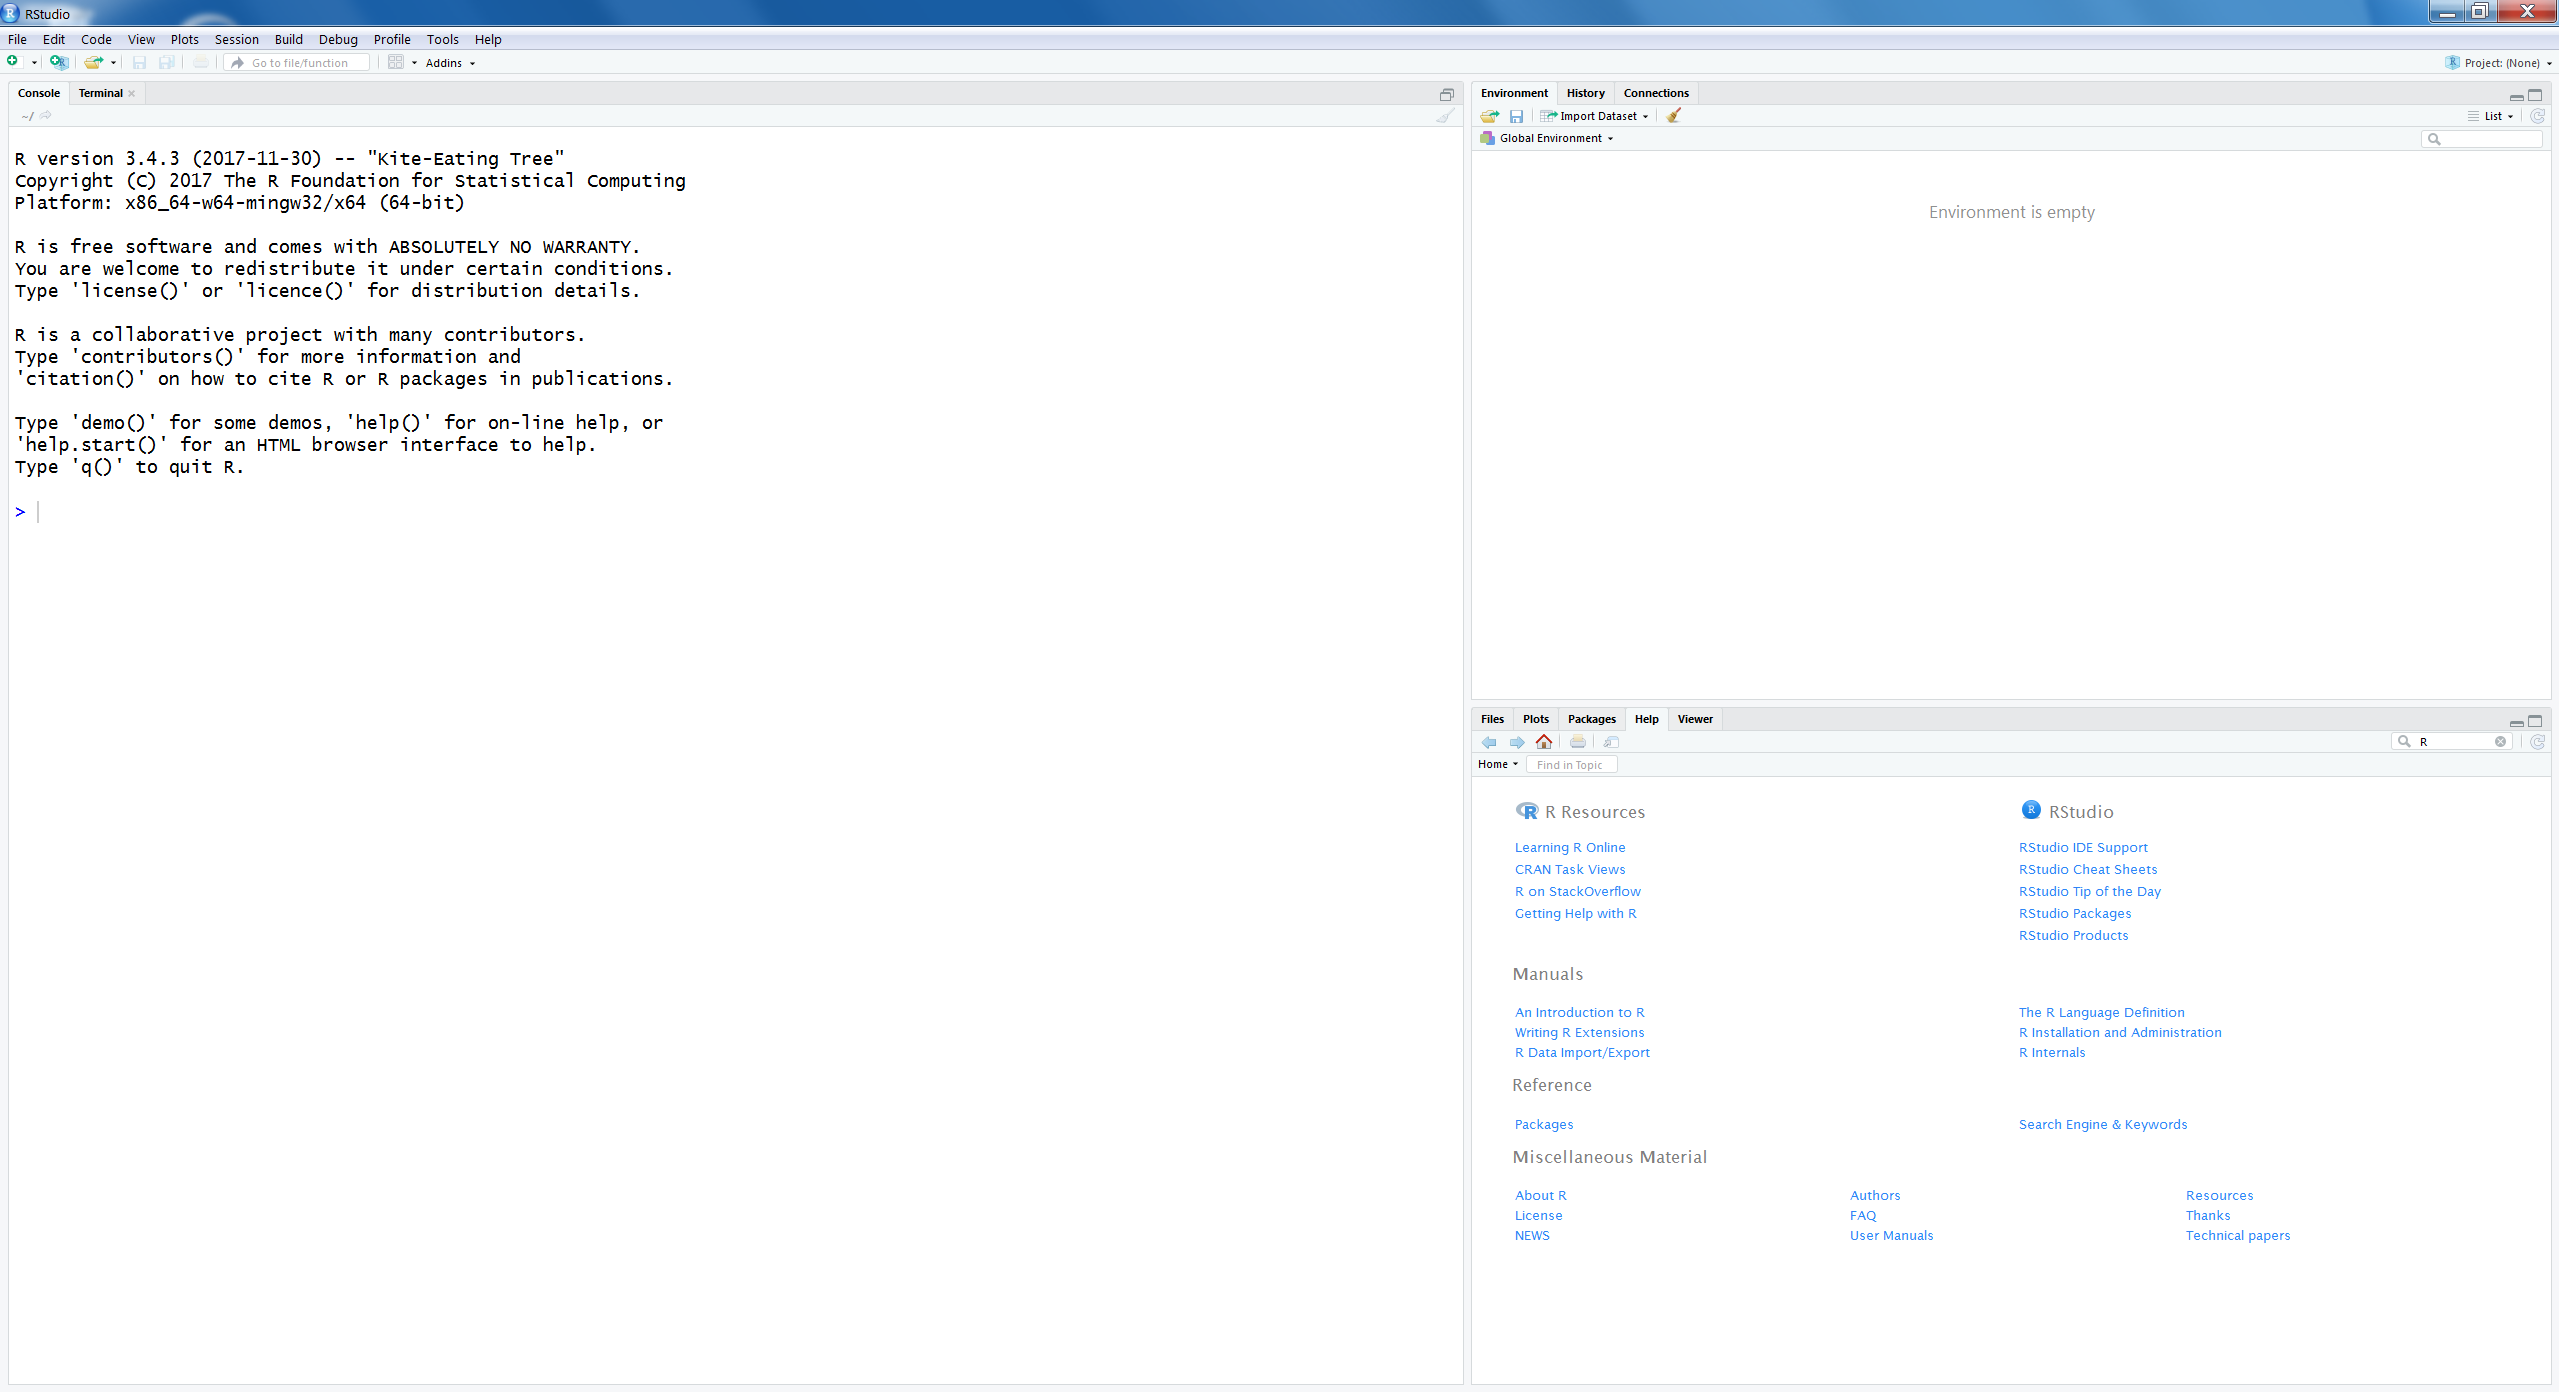
\includegraphics[width=0.9\linewidth]{images/fig1.10} 

}

\caption{First screen that appears after you have started RStudio}\label{fig:fig10}
\end{figure}

There are three windows opened:

\begin{enumerate}
\def\labelenumi{\arabic{enumi}.}
\tightlist
\item
  On the left is the Console window
\end{enumerate}

This is the main window to run R code (see below for more information
about the Console window).

\begin{enumerate}
\def\labelenumi{\arabic{enumi}.}
\setcounter{enumi}{1}
\tightlist
\item
  Right above is the window where you can choose between the Environment
  and History tabs (e.g.~history tracks the code you typed in the
  Console window).
\item
  At the right site below is the window where you can choose between
  Files, Plots, Packages, Help and Viewer tabs.
\end{enumerate}

\subsection{The role of the Console
Window}\label{the-role-of-the-console-window}

When you enter code in the Console window you will directly receive a
result. For example, you can type the following code and the result will
appear directly in the Console window.

\begin{Shaded}
\begin{Highlighting}[]
\DecValTok{3} \OperatorTok{+}\StringTok{ }\DecValTok{3}
\end{Highlighting}
\end{Shaded}

\begin{verbatim}
## [1] 6
\end{verbatim}

As you can see, you can use R as a large calculator. Other
multiplication procedures as divide, square, etc. can also be executed.
However, the main use for R is its functions. For example, when you
generate 20 random numbers you can use the following function code (we
will discuss more about functions in R later):

\begin{Shaded}
\begin{Highlighting}[]
\KeywordTok{rnorm}\NormalTok{(}\DecValTok{20}\NormalTok{)}
\end{Highlighting}
\end{Shaded}

\begin{verbatim}
##  [1] -0.34856279 -0.90024815  1.63862714  1.17861626  0.03059941
##  [6] -1.19207296  0.93739296  0.09470795  1.22563277  0.12140848
## [11] -0.61991184  1.01064413 -1.18046004  0.01268044  2.58441690
## [16] -0.17549766 -0.21294877 -0.01599572  1.83793974 -1.59347635
\end{verbatim}

The number {[}1{]} between brackets is the index of the first number or
item in the vector. That can be useful when you have many numbers
printed in the Console window.

\subsection{R assignments and objects}\label{r-assignments-and-objects}

In R it is possible to create objects and to assign values to these
objects. In this way it is for example possible to store some
intermediate results and recall or use them later on. Assigning values
to objects is done by using the assignment operator \textless{}- (R code
below). You can also use the = sign as an assignment operator. This is
not recommended because this is also a symbol used for some mathematical
operations. For example, when we want to assign the value 3 to the
object x, we use the following code.

\begin{Shaded}
\begin{Highlighting}[]
\NormalTok{x <-}\StringTok{ }\DecValTok{3} 
\end{Highlighting}
\end{Shaded}

When we subsequently type in the letter x we get the following result:

\begin{Shaded}
\begin{Highlighting}[]
\NormalTok{x }
\end{Highlighting}
\end{Shaded}

\begin{verbatim}
## [1] 3
\end{verbatim}

As result we see the value 3 again. Now the value 3 is assigned to the
object x. In R all kind of information can be assigned to an object,
i.e.~one number, a vector of numbers, results from analysis or other R
objects such as data frames, matrices or lists. Objects can have all
kinds of different names, composed of different letters and numbers.
Here are some examples where number 3 is assigned to different objects
with different names:

\begin{Shaded}
\begin{Highlighting}[]
\NormalTok{test <-}\StringTok{ }\DecValTok{3}
\NormalTok{test.}\DecValTok{1}\NormalTok{ <-}\StringTok{ }\DecValTok{3}
\NormalTok{test.manual <-}\StringTok{ }\DecValTok{3}
\NormalTok{test}
\end{Highlighting}
\end{Shaded}

\begin{verbatim}
## [1] 3
\end{verbatim}

\begin{Shaded}
\begin{Highlighting}[]
\NormalTok{test.}\DecValTok{1}
\end{Highlighting}
\end{Shaded}

\begin{verbatim}
## [1] 3
\end{verbatim}

\begin{Shaded}
\begin{Highlighting}[]
\NormalTok{test.manual }
\end{Highlighting}
\end{Shaded}

\begin{verbatim}
## [1] 3
\end{verbatim}

Note that some letters and words are used by R itself. It is not
recommended to use these leters as names for objects in R that you
create yourself. For example, the letter T and F are used as TRUE and
FALSE by R. Other letters that are already in use are c, q, t, C, D, I
and diff, df, and pt.

\subsection{Vectors, matrices, lists and data
frames}\label{vectors-matrices-lists-and-data-frames}

\emph{Vectors} In the previous paragraph we created the one-vector x,
i.e.~a vector that contained only one number, the number 3. Mostly you
do your analysis on more numbers than just one. R has several
possibilities to create objects with more data. We start with a simple
dataset, called a data vector, which is an array of numbers (such as
created in R code 1.2. A vector can be created by the following code:

\begin{Shaded}
\begin{Highlighting}[]
\NormalTok{y <-}\StringTok{ }\KeywordTok{c}\NormalTok{(}\DecValTok{1}\NormalTok{, }\DecValTok{2}\NormalTok{, }\DecValTok{3}\NormalTok{, }\DecValTok{4}\NormalTok{, }\DecValTok{5}\NormalTok{)}
\NormalTok{y}
\end{Highlighting}
\end{Shaded}

\begin{verbatim}
## [1] 1 2 3 4 5
\end{verbatim}

Now the numbers 1, 2, 3, 4 and 5 are assigned to the data vector y. The
``c'' in the above code stand for concatenate which makes that all
separate (one-vector) numbers are merged into one vector. It is also
possible to create character vectors, which are vectors that contain
strings (text). An example:

\begin{Shaded}
\begin{Highlighting}[]
\NormalTok{y <-}\StringTok{ }\KeywordTok{c}\NormalTok{(}\StringTok{"a"}\NormalTok{, }\StringTok{"b"}\NormalTok{, }\StringTok{"test"}\NormalTok{)}
\NormalTok{y}
\end{Highlighting}
\end{Shaded}

\begin{verbatim}
## [1] "a"    "b"    "test"
\end{verbatim}

Vectors can also be made by using the ``:'' symbol. With that symbol it
is easy to generate a sequence of numbers. An example:

\begin{Shaded}
\begin{Highlighting}[]
\NormalTok{y <-}\StringTok{ }\DecValTok{1}\OperatorTok{:}\DecValTok{10}
\NormalTok{y}
\end{Highlighting}
\end{Shaded}

\begin{verbatim}
##  [1]  1  2  3  4  5  6  7  8  9 10
\end{verbatim}

\begin{Shaded}
\begin{Highlighting}[]
\NormalTok{y <-}\StringTok{ }\DecValTok{2}\OperatorTok{:}\DecValTok{6}
\NormalTok{y}
\end{Highlighting}
\end{Shaded}

\begin{verbatim}
## [1] 2 3 4 5 6
\end{verbatim}

Both lines of code produce a vector containing a sequence of numbers.
The first example produces the numbers 1 to 10 and the second example
the numbers 2 to 6.

\emph{Matrix} A matrix in R contains rows and columns and can be created
by using the matrix function.

\begin{Shaded}
\begin{Highlighting}[]
\KeywordTok{matrix}\NormalTok{(}\KeywordTok{c}\NormalTok{(}\DecValTok{1}\NormalTok{, }\DecValTok{2}\NormalTok{, }\DecValTok{3}\NormalTok{, }\DecValTok{4}\NormalTok{, }\DecValTok{5}\NormalTok{, }\DecValTok{6}\NormalTok{), }\DataTypeTok{nrow=}\DecValTok{2}\NormalTok{, }\DataTypeTok{ncol=}\DecValTok{3}\NormalTok{)}
\end{Highlighting}
\end{Shaded}

\begin{verbatim}
##      [,1] [,2] [,3]
## [1,]    1    3    5
## [2,]    2    4    6
\end{verbatim}

Now we have created a matrix with 2 rows and 3 columns. In essence we
converted the vector c(1, 2, 3, 4, 5, 6) into a matrix.

\emph{List} Another popular R object class is a list. The advantage of a
list is that it can contain components of different formats. Let's look
at an example using the following code:

\begin{Shaded}
\begin{Highlighting}[]
\NormalTok{x <-}\StringTok{ }\DecValTok{1}\OperatorTok{:}\DecValTok{5}
\NormalTok{x}
\end{Highlighting}
\end{Shaded}

\begin{verbatim}
## [1] 1 2 3 4 5
\end{verbatim}

\begin{Shaded}
\begin{Highlighting}[]
\NormalTok{y <-}\StringTok{ }\KeywordTok{c}\NormalTok{(}\StringTok{"a"}\NormalTok{, }\StringTok{"b"}\NormalTok{, }\StringTok{"test"}\NormalTok{)}
\NormalTok{z <-}\StringTok{ }\KeywordTok{list}\NormalTok{(}\DataTypeTok{x=}\NormalTok{x, }\DataTypeTok{y=}\NormalTok{y)}
\NormalTok{z}
\end{Highlighting}
\end{Shaded}

\begin{verbatim}
## $x
## [1] 1 2 3 4 5
## 
## $y
## [1] "a"    "b"    "test"
\end{verbatim}

The code created the list object z consisting of the two components x
and y which are the vectors that were created above. You can see that in
a list two components of different data type can be combined, a numeric
and a character factor. The names of the list components are indicated
by the dollar sign,
\(. The list component can be obtained separately by typing z\)x for
component x or x\$y for component y.

\emph{Dataframe} Mostly we work with datasets that contain information
of different variables and persons. In R such a dataset is called a
dataframe. In essence, a dataframe in R is a list, where each component
of the list is a vector of equal length. This example code first creates
a list, consisting of 3 vectors of the same length. Than this list is
converted into a dataframe, using the data.frame function.

\begin{Shaded}
\begin{Highlighting}[]
\NormalTok{k <-}\StringTok{ }\KeywordTok{list}\NormalTok{(}\DataTypeTok{a=}\DecValTok{1}\OperatorTok{:}\DecValTok{10}\NormalTok{, }\DataTypeTok{b=}\DecValTok{11}\OperatorTok{:}\DecValTok{20}\NormalTok{, }\DataTypeTok{c=}\DecValTok{21}\OperatorTok{:}\DecValTok{30}\NormalTok{)}
\NormalTok{k}
\end{Highlighting}
\end{Shaded}

\begin{verbatim}
## $a
##  [1]  1  2  3  4  5  6  7  8  9 10
## 
## $b
##  [1] 11 12 13 14 15 16 17 18 19 20
## 
## $c
##  [1] 21 22 23 24 25 26 27 28 29 30
\end{verbatim}

\begin{Shaded}
\begin{Highlighting}[]
\NormalTok{z <-}\StringTok{ }\KeywordTok{data.frame}\NormalTok{(k)}
\NormalTok{z}
\end{Highlighting}
\end{Shaded}

\begin{verbatim}
##     a  b  c
## 1   1 11 21
## 2   2 12 22
## 3   3 13 23
## 4   4 14 24
## 5   5 15 25
## 6   6 16 26
## 7   7 17 27
## 8   8 18 28
## 9   9 19 29
## 10 10 20 30
\end{verbatim}

Typically, a dataframe is created by reading in an existing dataset. How
to create a dataframe by reading in a dataset will be further discussed
in the paragraph ``Reading in and saving data''.

\subsection{Indexing Vectors, Matrices, Lists and Data
frames}\label{indexing-vectors-matrices-lists-and-data-frames}

\emph{Vectors} An important operation in R is to select a subset of a
given vector. This is called indexing vectors. This subset of the vector
elements can be assigned to another vector. An example how to do this:

\begin{Shaded}
\begin{Highlighting}[]
\NormalTok{y <-}\StringTok{ }\KeywordTok{c}\NormalTok{(}\DecValTok{3}\NormalTok{, }\DecValTok{5}\NormalTok{, }\DecValTok{2}\NormalTok{, }\DecValTok{8}\NormalTok{, }\DecValTok{5}\NormalTok{, }\DecValTok{4}\NormalTok{, }\DecValTok{8}\NormalTok{, }\DecValTok{1}\NormalTok{, }\DecValTok{3}\NormalTok{, }\DecValTok{6}\NormalTok{)}
\NormalTok{y[}\KeywordTok{c}\NormalTok{(}\DecValTok{1}\NormalTok{, }\DecValTok{4}\NormalTok{)]}
\end{Highlighting}
\end{Shaded}

\begin{verbatim}
## [1] 3 8
\end{verbatim}

The R code y{[}c(1, 4){]}, extracts the first and fourth element of the
vector. Another example is by using the ``:'' symbol, to extract several
subsequent elements:

\begin{Shaded}
\begin{Highlighting}[]
\NormalTok{y[}\DecValTok{2}\OperatorTok{:}\DecValTok{5}\NormalTok{]}
\end{Highlighting}
\end{Shaded}

\begin{verbatim}
## [1] 5 2 8 5
\end{verbatim}

The R code y{[}2:5{]}, extracts the second to the fifth element of the
vector.

A minus sign excludes the specific element from the vector, like:

\begin{Shaded}
\begin{Highlighting}[]
\NormalTok{y[}\OperatorTok{-}\DecValTok{3}\NormalTok{]}
\end{Highlighting}
\end{Shaded}

\begin{verbatim}
## [1] 3 5 8 5 4 8 1 3 6
\end{verbatim}

The R code y{[}-3{]}, excludes the third element of the vector (i.e.~2).
A new vector z can be created where the third and fourth element of the
y vector are excluded, by using the following code:

\begin{Shaded}
\begin{Highlighting}[]
\NormalTok{z <-}\StringTok{ }\NormalTok{y[}\OperatorTok{-}\KeywordTok{c}\NormalTok{(}\DecValTok{3}\NormalTok{, }\DecValTok{4}\NormalTok{)]}
\NormalTok{z}
\end{Highlighting}
\end{Shaded}

\begin{verbatim}
## [1] 3 5 5 4 8 1 3 6
\end{verbatim}

\emph{Matrices} When we index matrices we can choose to index rows,
columns or both. Here are some examples:

First we construct the matrix

\begin{Shaded}
\begin{Highlighting}[]
\NormalTok{z <-}\StringTok{ }\KeywordTok{matrix}\NormalTok{(}\DecValTok{1}\OperatorTok{:}\DecValTok{9}\NormalTok{, }\DataTypeTok{nrow=}\DecValTok{3}\NormalTok{)}
\NormalTok{z}
\end{Highlighting}
\end{Shaded}

\begin{verbatim}
##      [,1] [,2] [,3]
## [1,]    1    4    7
## [2,]    2    5    8
## [3,]    3    6    9
\end{verbatim}

We extract from the first row the number in the second column

\begin{Shaded}
\begin{Highlighting}[]
\NormalTok{z[}\DecValTok{1}\NormalTok{, }\DecValTok{2}\NormalTok{]}
\end{Highlighting}
\end{Shaded}

\begin{verbatim}
## [1] 4
\end{verbatim}

We extract all numbers in each column in the first row

\begin{Shaded}
\begin{Highlighting}[]
\NormalTok{z[}\DecValTok{1}\NormalTok{, ]}
\end{Highlighting}
\end{Shaded}

\begin{verbatim}
## [1] 1 4 7
\end{verbatim}

We extract all numbers in each row of the first column

\begin{Shaded}
\begin{Highlighting}[]
\NormalTok{z[, }\DecValTok{1}\NormalTok{]}
\end{Highlighting}
\end{Shaded}

\begin{verbatim}
## [1] 1 2 3
\end{verbatim}

A minus sign can also be used to delete specific elements or complete
rows or columns.

Omit the first row from the matrix

\begin{Shaded}
\begin{Highlighting}[]
\NormalTok{z[}\OperatorTok{-}\DecValTok{1}\NormalTok{, ]}
\end{Highlighting}
\end{Shaded}

\begin{verbatim}
##      [,1] [,2] [,3]
## [1,]    2    5    8
## [2,]    3    6    9
\end{verbatim}

\emph{Lists} We first create a list with 3 components, each component
consists of a vector of the same length and with 10 elements each.

\begin{Shaded}
\begin{Highlighting}[]
\NormalTok{k <-}\StringTok{ }\KeywordTok{list}\NormalTok{(}\DataTypeTok{a=}\DecValTok{1}\OperatorTok{:}\DecValTok{10}\NormalTok{, }\DataTypeTok{b=}\DecValTok{11}\OperatorTok{:}\DecValTok{20}\NormalTok{, }\DataTypeTok{c=}\DecValTok{21}\OperatorTok{:}\DecValTok{30}\NormalTok{)}
\NormalTok{k}
\end{Highlighting}
\end{Shaded}

\begin{verbatim}
## $a
##  [1]  1  2  3  4  5  6  7  8  9 10
## 
## $b
##  [1] 11 12 13 14 15 16 17 18 19 20
## 
## $c
##  [1] 21 22 23 24 25 26 27 28 29 30
\end{verbatim}

There are several options to index list components and elements of the
components. If we want to index the individual component b we can use
the following code:

\begin{Shaded}
\begin{Highlighting}[]
\NormalTok{k}\OperatorTok{$}\NormalTok{b}
\end{Highlighting}
\end{Shaded}

\begin{verbatim}
##  [1] 11 12 13 14 15 16 17 18 19 20
\end{verbatim}

\begin{Shaded}
\begin{Highlighting}[]
\NormalTok{k[[}\StringTok{"b"}\NormalTok{]]}
\end{Highlighting}
\end{Shaded}

\begin{verbatim}
##  [1] 11 12 13 14 15 16 17 18 19 20
\end{verbatim}

\begin{Shaded}
\begin{Highlighting}[]
\NormalTok{k[[}\DecValTok{2}\NormalTok{]]}
\end{Highlighting}
\end{Shaded}

\begin{verbatim}
##  [1] 11 12 13 14 15 16 17 18 19 20
\end{verbatim}

As you have may noticed, to extract individual list components double
square brackets are used, compared to single brackets for indexing
vectors and matrices.

When we use single brackets, we get the following results:

\begin{Shaded}
\begin{Highlighting}[]
\NormalTok{k[}\StringTok{"b"}\NormalTok{]}
\end{Highlighting}
\end{Shaded}

\begin{verbatim}
## $b
##  [1] 11 12 13 14 15 16 17 18 19 20
\end{verbatim}

The difference between using single and double brackets is that single
brackets return the component data type, which is in this case a vector
(but could be any kind of data type) and single brackets always return a
list.

\emph{Data frames} Indexing data frames follows the same method as
indexing matrices, but we can also use the method that is used to index
lists, since data frames are essentially lists of vectors of the same
length. Data frames consist of rows and columns which can be accessed
separately or both to extract specific elements. We use the data frame
that was constructed in R code 1.11.

\begin{Shaded}
\begin{Highlighting}[]
\NormalTok{z}
\end{Highlighting}
\end{Shaded}

\begin{verbatim}
##      [,1] [,2] [,3]
## [1,]    1    4    7
## [2,]    2    5    8
## [3,]    3    6    9
\end{verbatim}

Examples of indexing the first column are:

\begin{Shaded}
\begin{Highlighting}[]
\NormalTok{z[, }\DecValTok{1}\NormalTok{]}
\end{Highlighting}
\end{Shaded}

\begin{verbatim}
## [1] 1 2 3
\end{verbatim}

\begin{Shaded}
\begin{Highlighting}[]
\NormalTok{k}\OperatorTok{$}\NormalTok{a}
\end{Highlighting}
\end{Shaded}

\begin{verbatim}
##  [1]  1  2  3  4  5  6  7  8  9 10
\end{verbatim}

The second row can be accessed by using:

\begin{Shaded}
\begin{Highlighting}[]
\NormalTok{z[}\DecValTok{2}\NormalTok{, ]}
\end{Highlighting}
\end{Shaded}

\begin{verbatim}
## [1] 2 5 8
\end{verbatim}

\subsection{Vectorized Calculation}\label{vectorized-calculation}

An advantage of working with R is that it is possible to perform
vectorized calculations. This means that you can do calculations
elementwise, i.e.~the same calculation is done on each element of an
object. Let's look at an example.

We first create a vector z with numerical variables.

\begin{Shaded}
\begin{Highlighting}[]
\NormalTok{z <-}\StringTok{ }\KeywordTok{c}\NormalTok{(}\DecValTok{1}\NormalTok{, }\DecValTok{2}\NormalTok{, }\DecValTok{3}\NormalTok{, }\DecValTok{4}\NormalTok{, }\DecValTok{5}\NormalTok{, }\DecValTok{6}\NormalTok{, }\DecValTok{7}\NormalTok{, }\DecValTok{8}\NormalTok{)}
\NormalTok{z}
\end{Highlighting}
\end{Shaded}

\begin{verbatim}
## [1] 1 2 3 4 5 6 7 8
\end{verbatim}

Now it is fairly easy to square each element of the vector by typing:

\begin{Shaded}
\begin{Highlighting}[]
\NormalTok{z}\OperatorTok{^}\DecValTok{2}
\end{Highlighting}
\end{Shaded}

\begin{verbatim}
## [1]  1  4  9 16 25 36 49 64
\end{verbatim}

The \^{}2 means take the power of 2. We see that each element is
squared. These vectorized calculations can be done by using all kinds of
mathematical functions, e.g.~taking the square root, logarithms, adding
constant values to each element, etc.

\subsection{R Functions}\label{r-functions}

Functions play an important role in R. Functions can be seen as lines of
R code to run all kind of data procedures and to return a result. Let's
write a small function that we name ``sum.test'' that generates a
sequence of numbers from 1 to 5 and sums all values from 1 to the value
we define beforehand, which is in our example the value 3. This means
that the function will sum all values from 1 to 3, i.e.~1 + 2 + 3 when
it is at the value of 3 and all values from 1 to 4 when we use as input
value the value 4. The function can be found in R code 1.26.

\begin{Shaded}
\begin{Highlighting}[]
\NormalTok{print.sum.test <-}\StringTok{ }\ControlFlowTok{function}\NormalTok{(x) }
\NormalTok{\{}
 \ControlFlowTok{for}\NormalTok{ (i }\ControlFlowTok{in} \DecValTok{1}\OperatorTok{:}\DecValTok{5}\NormalTok{) }
\NormalTok{ \{}
   \ControlFlowTok{if}\NormalTok{ (i}\OperatorTok{==}\NormalTok{x) y <-}\StringTok{ }\KeywordTok{sum}\NormalTok{(}\DecValTok{1}\OperatorTok{:}\NormalTok{i)  }
\NormalTok{ \}}
\KeywordTok{return}\NormalTok{(y)}
\NormalTok{\}}
\KeywordTok{print.sum.test}\NormalTok{(}\DecValTok{3}\NormalTok{)}
\end{Highlighting}
\end{Shaded}

\begin{verbatim}
## [1] 6
\end{verbatim}

At the first line we define the function print.sum.test that includes
one argument x. Than in de body of the function (in italic) which starts
with a left brace and ends with another brace, the actual calculations
take place. The return statement gives back the result. At the end we
call the function with the statement print.sum.test(3), where the value
3 is actually used in the function.

Once the function is defined, we can call the function and plug in other
values. For example:

\begin{Shaded}
\begin{Highlighting}[]
\KeywordTok{print.sum.test}\NormalTok{(}\DecValTok{4}\NormalTok{)}
\end{Highlighting}
\end{Shaded}

\begin{verbatim}
## [1] 10
\end{verbatim}

That will directly lead to the result 10 when the value 4 is used.

You can write functions yourself but in R many functions are available
which means that many calculations are done by using function calls. A
function name is followed by a set of parentheses which contain some
arguments. In the above self-written function, we already made use of a
function, which is the sum function. We can use it separately as
follows:

\begin{Shaded}
\begin{Highlighting}[]
\KeywordTok{sum}\NormalTok{(}\DecValTok{3}\NormalTok{,}\DecValTok{4}\NormalTok{)}
\end{Highlighting}
\end{Shaded}

\begin{verbatim}
## [1] 7
\end{verbatim}

The arguments in this function are the numbers 3 and 4 and the result is
their sum. This function uses as arguments numbers or complete vectors.
If you want to see the formal arguments of each function you can use the
args function. You have to type the name of the function as the argument
in the args function. For example, we can use it for the matrix
function:

\begin{Shaded}
\begin{Highlighting}[]
\KeywordTok{args}\NormalTok{(matrix)}
\end{Highlighting}
\end{Shaded}

\begin{verbatim}
## function (data = NA, nrow = 1, ncol = 1, byrow = FALSE, dimnames = NULL) 
## NULL
\end{verbatim}

As a result the arguments of the functions are listed with their default
settings. In this case the arguments are:

data: an optional data vector (including a list or expression vector).

nrow: the desired number of rows.

ncol: the desired number of columns.

byrow: logical. If FALSE (the default) the matrix is filled by columns,
otherwise the matrix is filled by rows.

dimnames: A dimnames attribute for the matrix: NULL or a list of length
2 giving the row and column names respectively. An empty list is treated
as NULL, and a list of length one as row names. The list can be named,
and the list names will be used as names for the dimensions.

\subsection{The Help function}\label{the-help-function}

There are several possibilities to start the help facilities in R and to
get more information about functions and their arguments in R.

You can just type help or use the question mark as follows:

help(matrix) ?matrix

In both ways the help tutorial for the matrix function will be activated
and appear in your web browser or in help tab in the right corner below
when you use R studio.

\subsection{Working with script files}\label{working-with-script-files}

If you want to use R code and functions more than once it is useful to
work with scripts files. In this way you can type and save R code and
reuse it. To create a script file in R is easy.

After you have started RStudio you go to File -\textgreater{} New File
-\textgreater{} R Scripts. Now a new window will open on the left side
above. In that file you can type for example the self-written function
print.sum.test. (Figure \ref{fig:fig11}). Now you can save the script
file by using the Save option under the File menu, open it again and use
it whenever you want.

\begin{figure}

{\centering 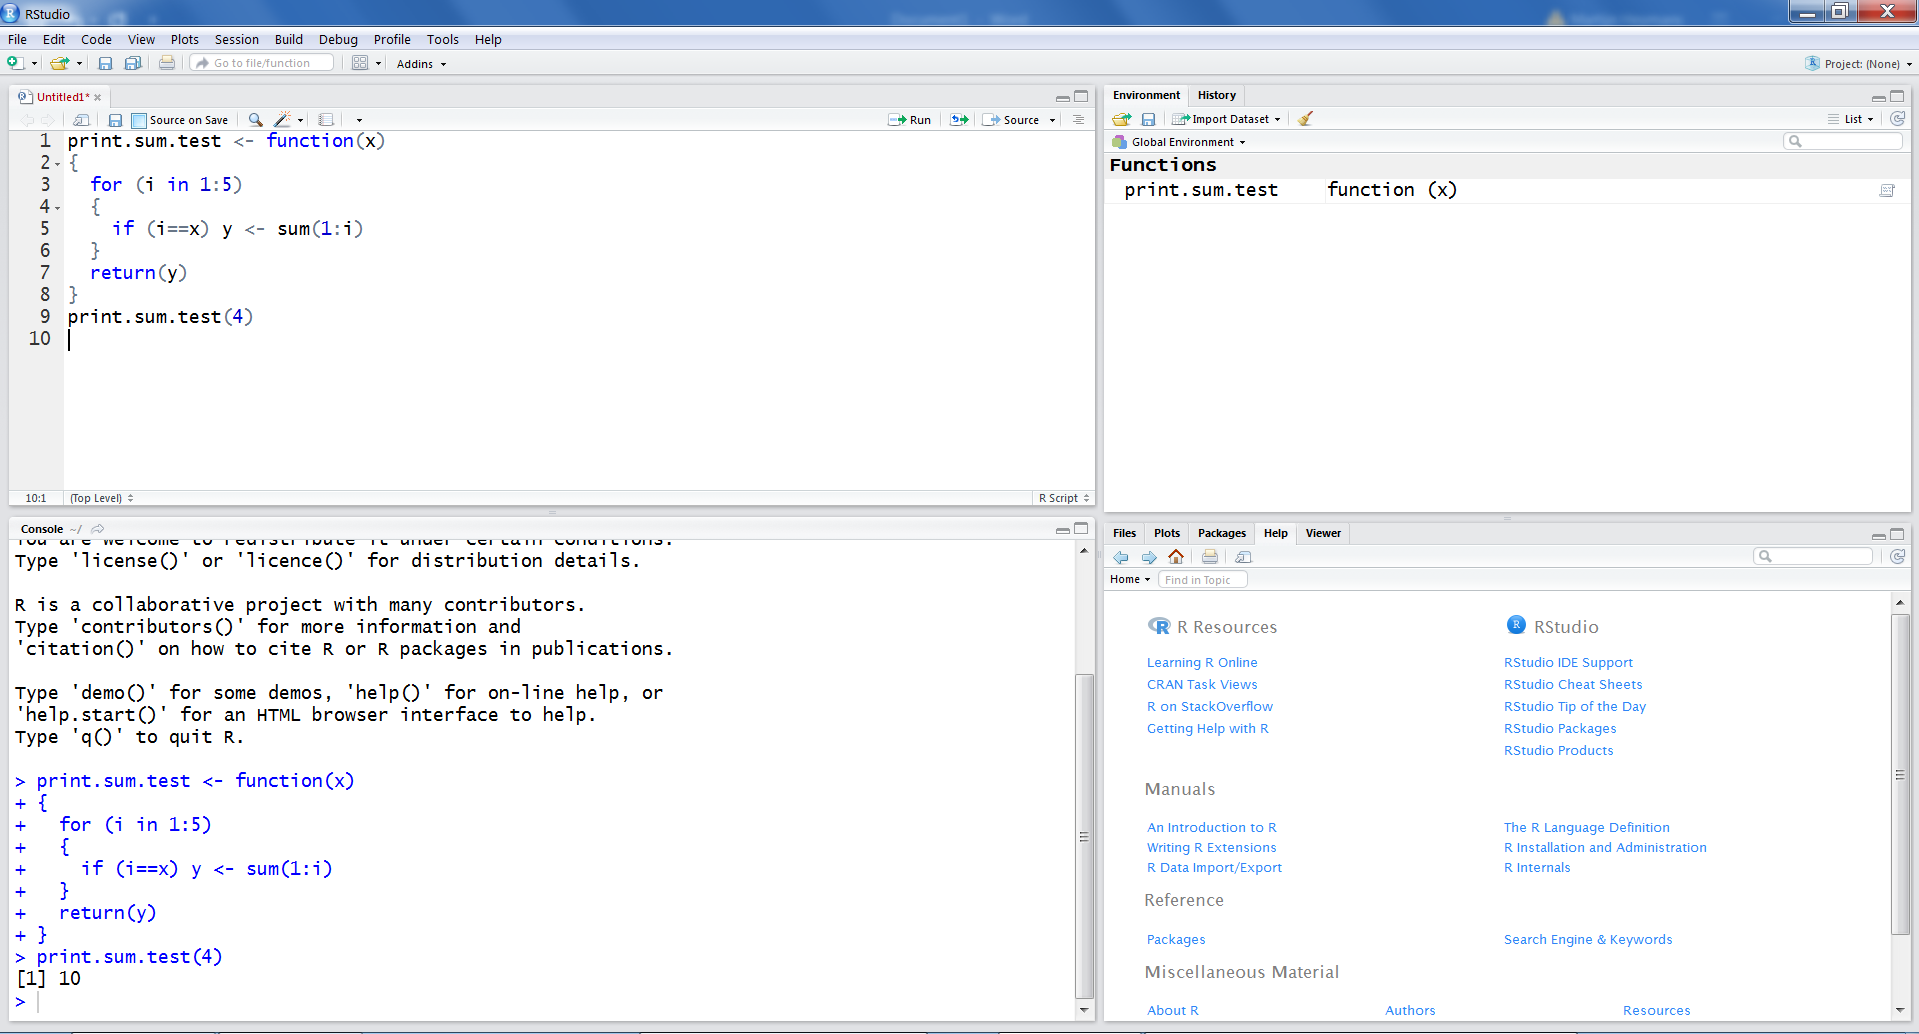
\includegraphics[width=0.9\linewidth]{images/fig1.11} 

}

\caption{Script file example in RStudio}\label{fig:fig11}
\end{figure}

\subsection{Creating a working
directory}\label{creating-a-working-directory}

It is a good idea to keep your R files at the same place when you are
doing data analysis for some kind of project. If you do not use a
separate directory, R will use a default directory, that will mostly be
in Windows in the documents folder. All files that you have to use
during your R session are assumed to be in that directory. Further, all
files that you save during your session will be in that directory. To
locate your working directory, you can type in the Console window:

If you want to change your working directory to for example
C:\Users\MWHeymans\Documents\R (Note that the path in R uses forward
slashes and the path in Windows backward slashes!), you can type:
\code{setwd("C:/Users/MWHeyamns/Documents/R")} \code{getwd()}

In Rstudio there is another way to get information about the current
working directory and another way to change the working directory. Go in
RStudio to the window on the right site below and go to the Files tab
and click on the right site of the screen on the three dots. Than a
window will open and you can browse to your preferred folder. Then
choose for More in the Files tab and then select ``Set As Working
Directory'' (Figure \ref{fig:fig12}). Now you have set your preferred
working directory. You can check if your directory is set correctly by
choosing ``Go To Working Directory''.

\begin{figure}

{\centering 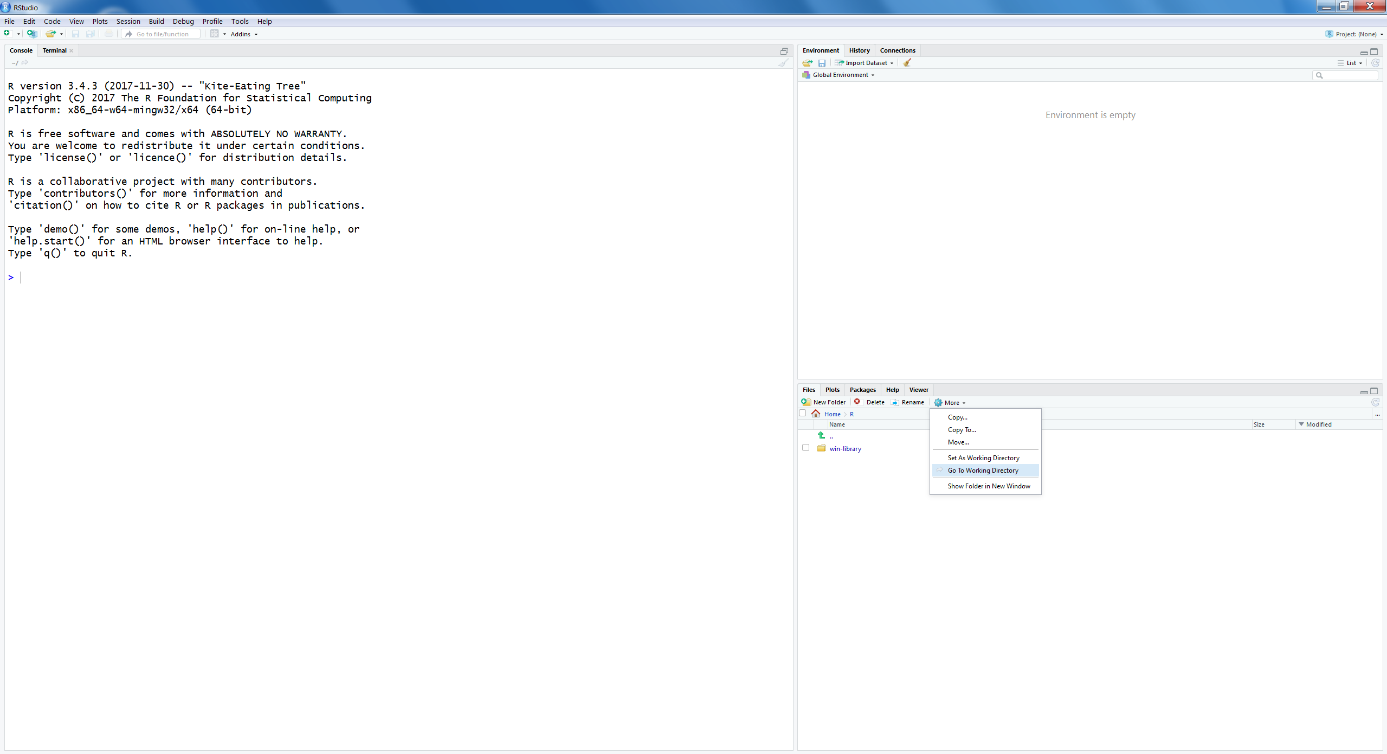
\includegraphics[width=0.9\linewidth]{images/fig1.12} 

}

\caption{Working directory selection in RStudio}\label{fig:fig12}
\end{figure}

\subsection{Reading in SPSS data in
RStudio}\label{reading-in-spss-data-in-rstudio}

There are several procedures in RStudio to read in datasets.

\begin{enumerate}
\def\labelenumi{\arabic{enumi}.}
\tightlist
\item
  Import datasets via ``Import Dataset'' An easy way to do that is via
  the window at the right site above. There you will find the button
  which is called ``Import Dataset''. When you click on it you can
  choose between different kind of file types, i.e.~CVS, Excel, SPSS,
  SAS and Stata files (Figure 1.13).
\end{enumerate}

\begin{figure}

{\centering 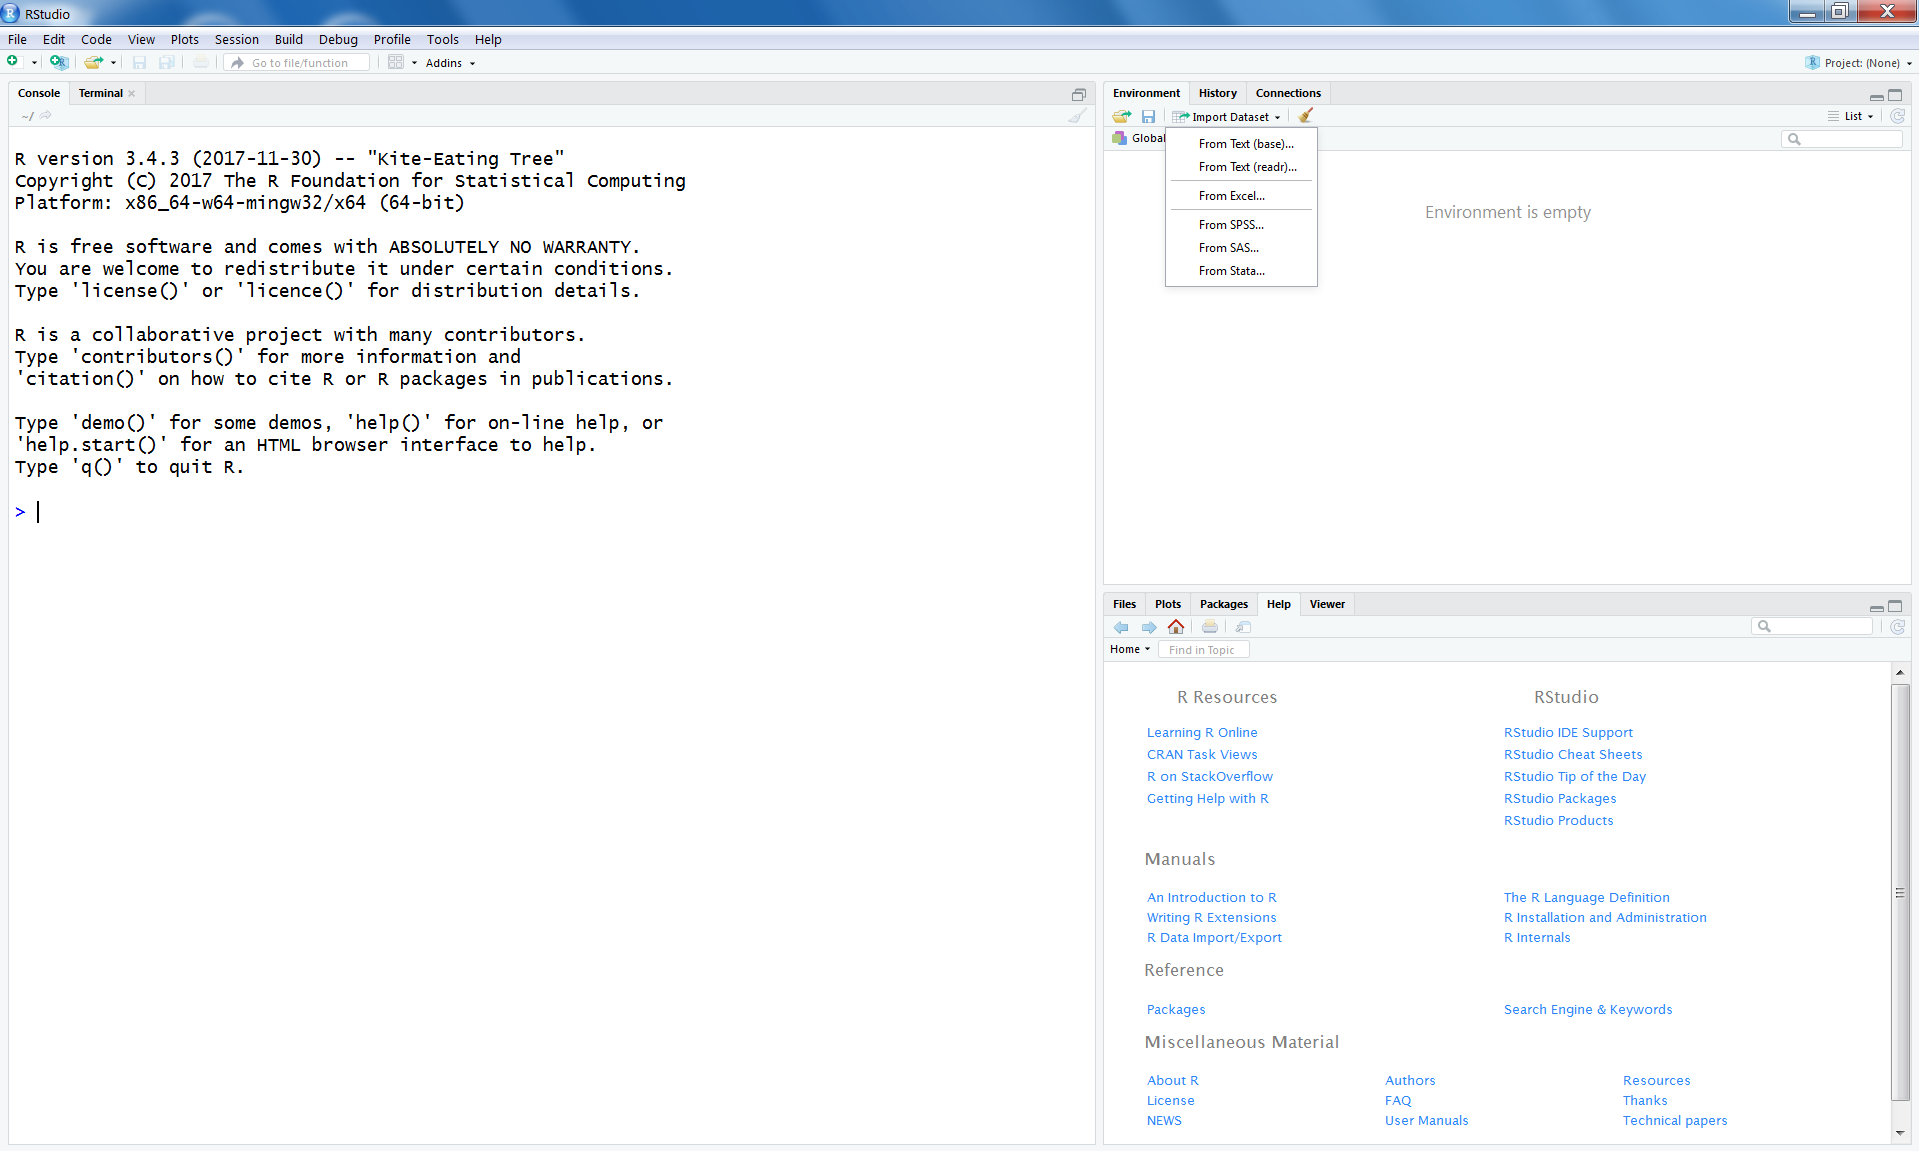
\includegraphics[width=0.9\linewidth]{images/fig1.13} 

}

\caption{Screen to import datasets in RStudio}\label{fig:fig13}
\end{figure}

In this example we choose for SPSS. When you approach this procedure for
the first time it could be that RStudio asks for your permission to
download a package called ``haven''. This package is built to import and
export data from several types. The following window will then appear
(Figure 1.14).

\begin{figure}

{\centering 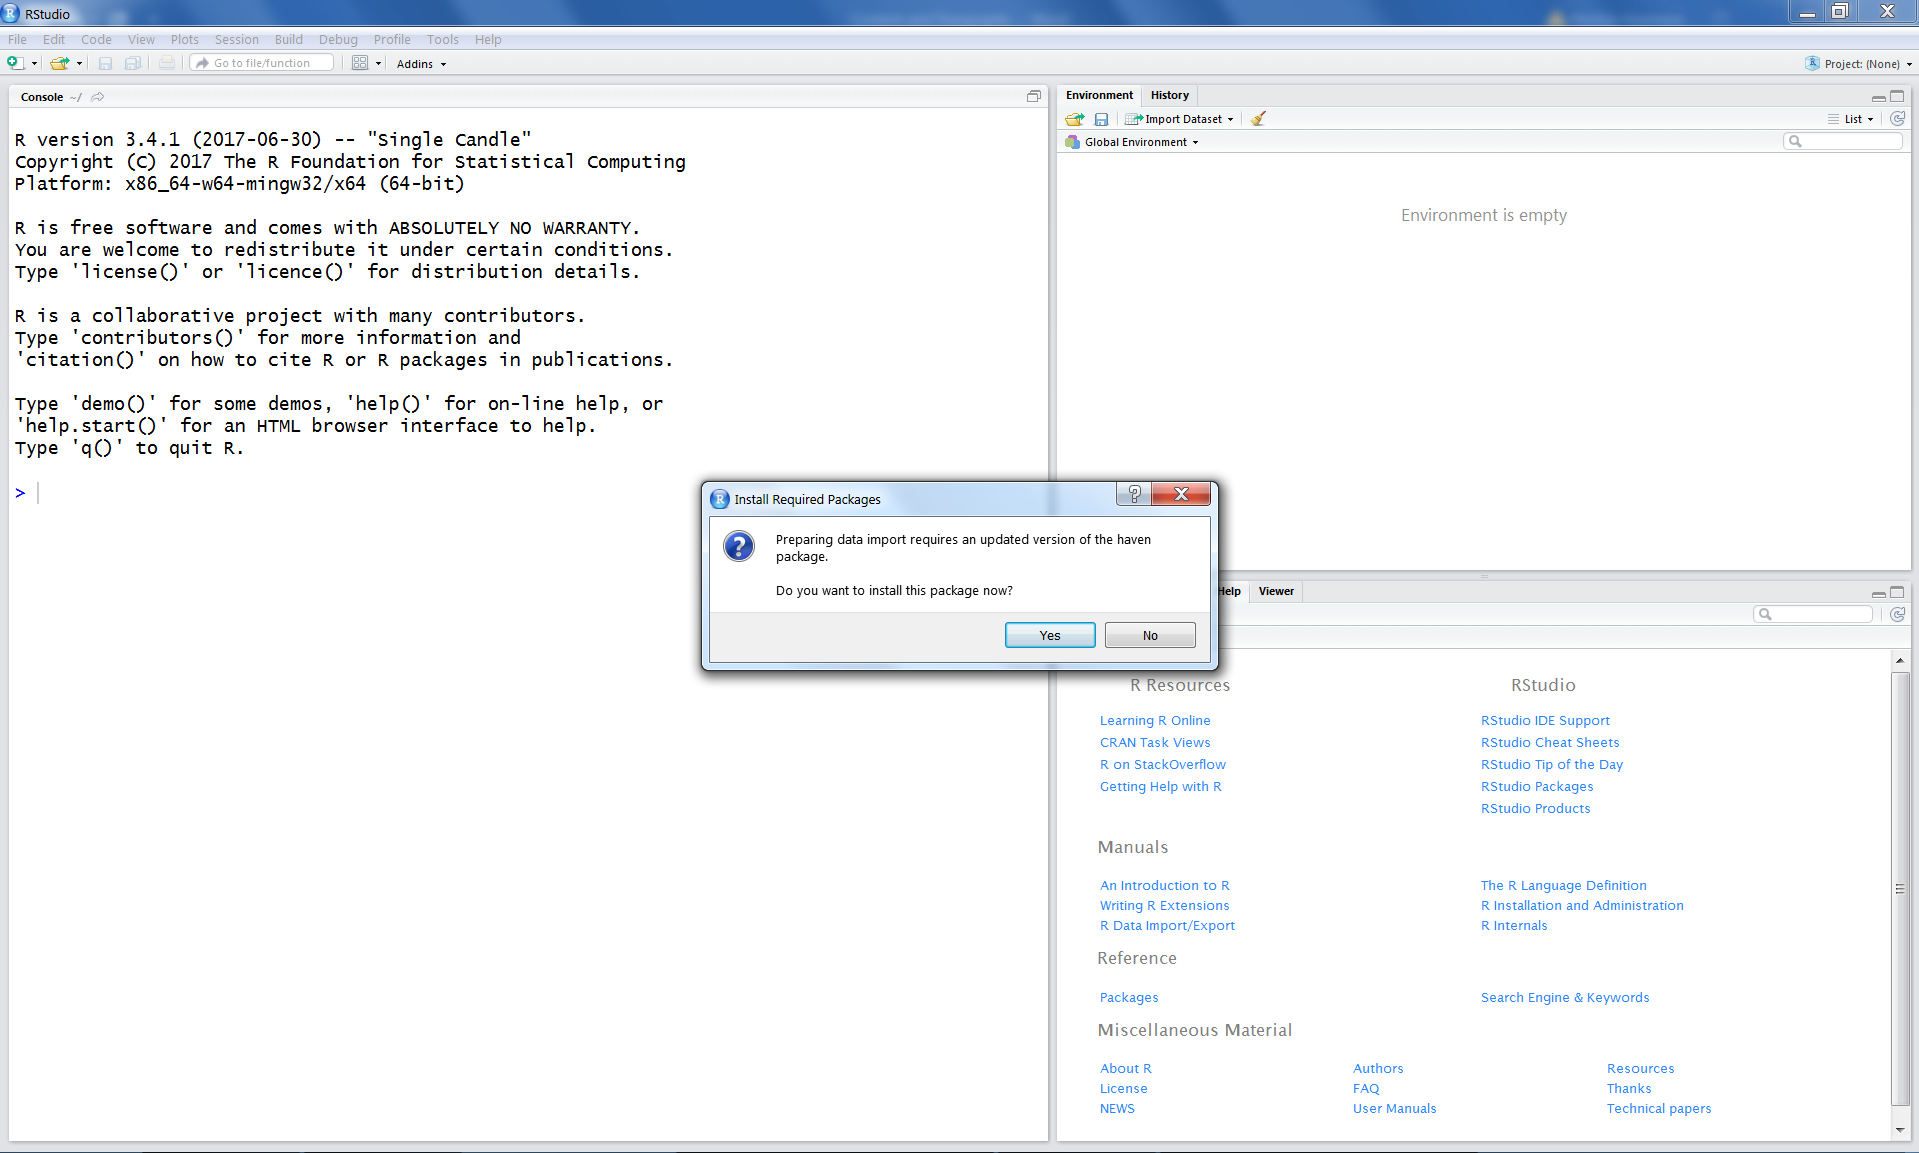
\includegraphics[width=0.9\linewidth]{images/fig1.14} 

}

\caption{Window to install the haven package}\label{fig:fig14}
\end{figure}

Click Yes and the download will start from the CRAN website. After the
package is installed a new window will open which is called ``Import
Statistical Data'' (Figure 1.15).

\begin{figure}

{\centering 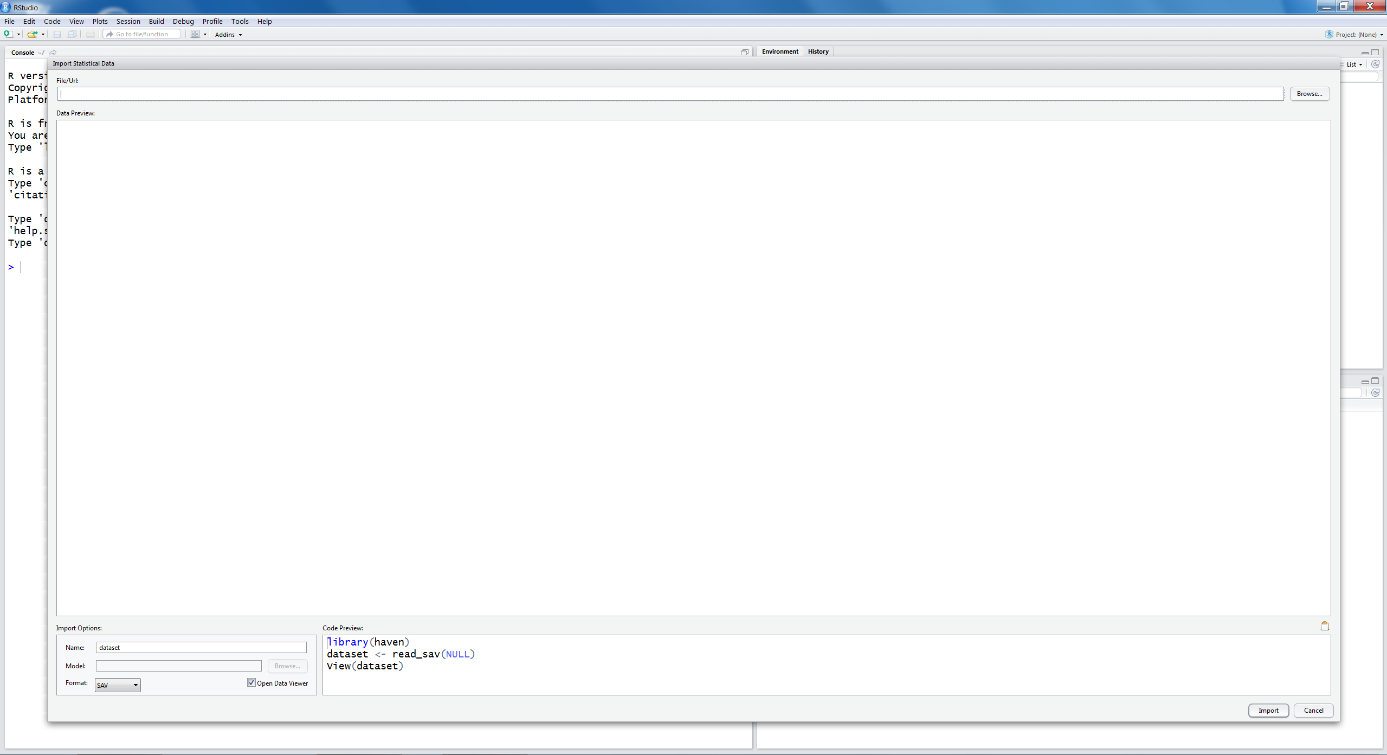
\includegraphics[width=0.9\linewidth]{images/fig1.15} 

}

\caption{The Import Statistical Data window in RStudio}\label{fig:fig15}
\end{figure}

At the top right site of the window you find the button which is called
``Browse''. That button allows you to browse to your dataset on your
computer. After you have opened your dataset you see a preview of your
dataset in RStudio (Figure 1.16).

\begin{figure}

{\centering 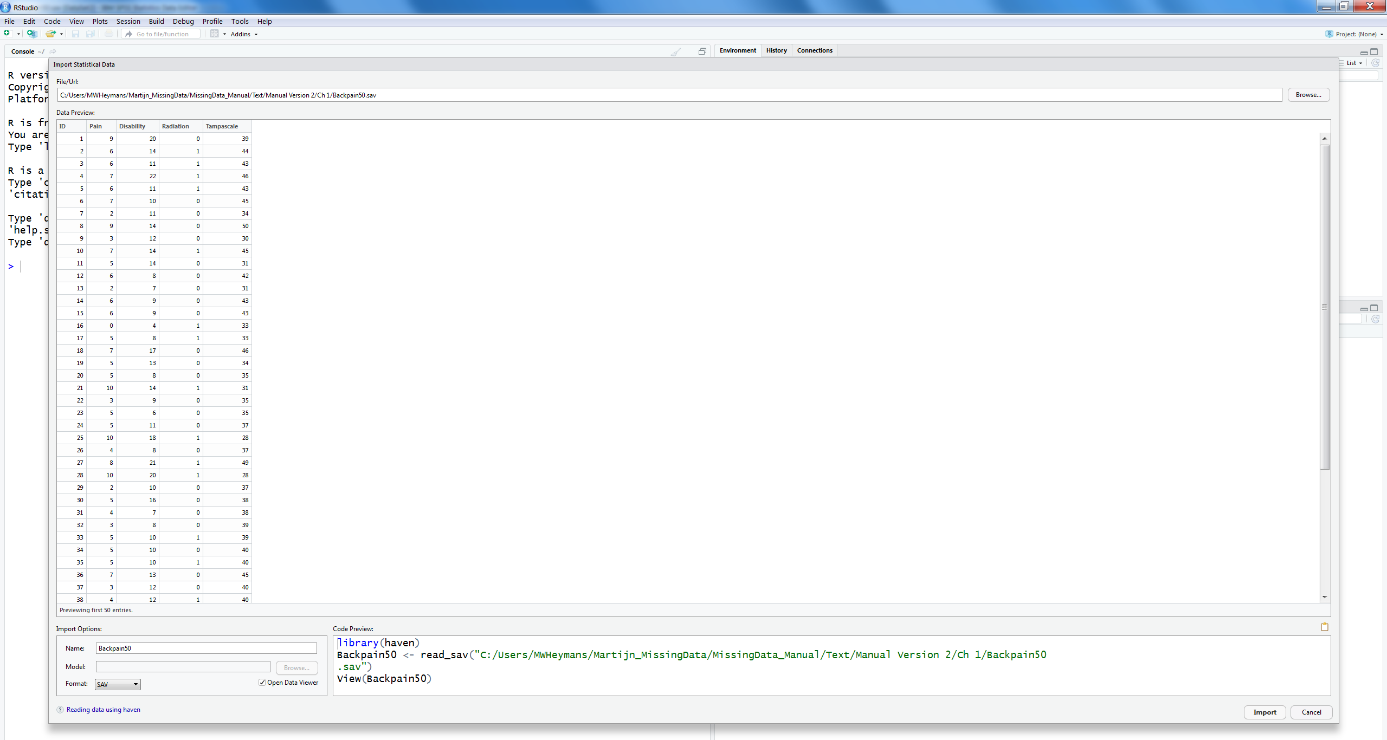
\includegraphics[width=0.9\linewidth]{images/fig1.16} 

}

\caption{A preview of the dataset in RStudio}\label{fig:fig16}
\end{figure}

Under Code Preview, under in the window, you see the code that was used
by RStudio to read in the dataset:

The dataset is automatically assigned to the object: Backpain50, which
is the original name of the dataset. When you click on Import, the
dataset is imported in the RStudio environment (Figure 1.17).

\begin{figure}

{\centering 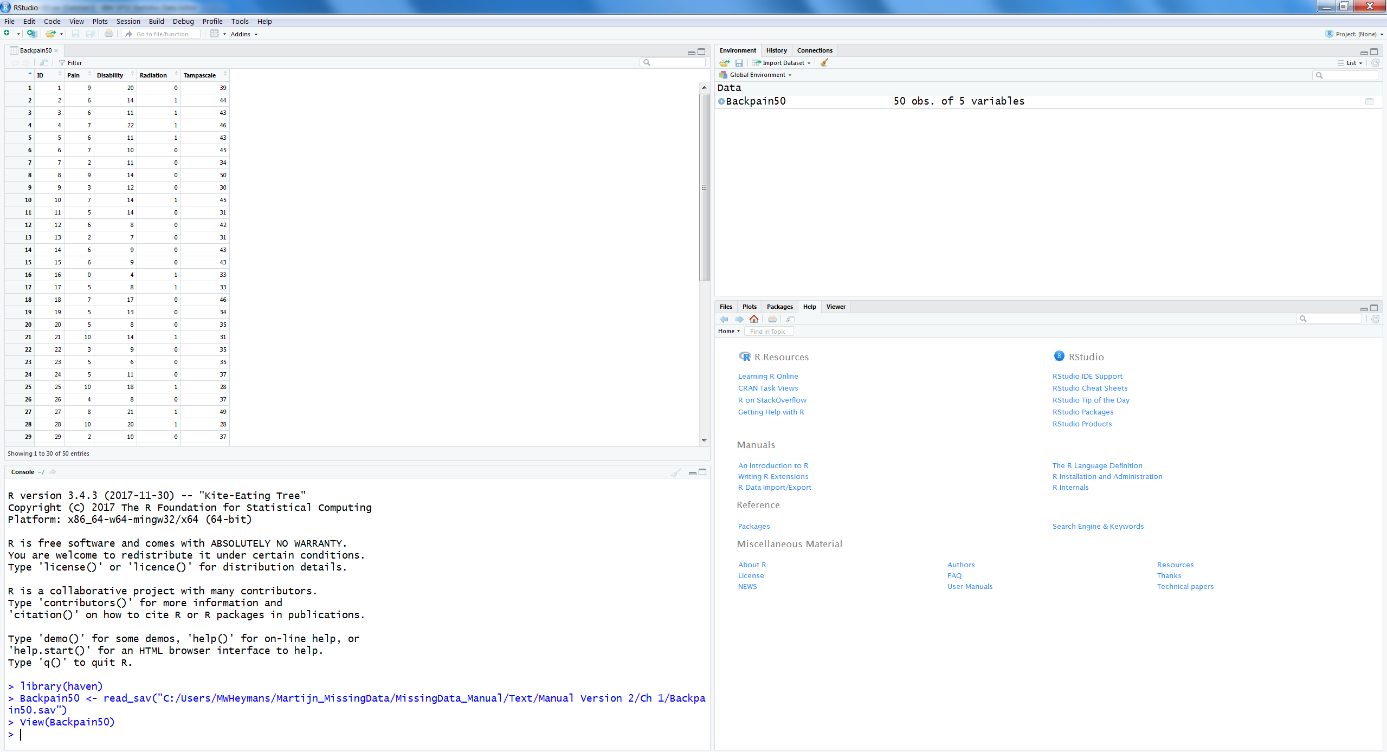
\includegraphics[width=0.9\linewidth]{images/fig1.17} 

}

\caption{Imported dataset in RStudio}\label{fig:fig17}
\end{figure}

Another way to import an SPSS dataset is by making use of the foreign
package. You can find this package under the Packages Tab in the window
at the right site below under the heading ``System Library''. Install
that package first. The foreign package includes the function
``read.spss''. Let's first explore the function arguments of this
function by using:

Now the following information can be found in the right window below,
under the Help tab:

read.spss(file, use.value.labels = TRUE, to.data.frame = FALSE,
max.value.labels = Inf, trim.factor.names = FALSE, trim\_values = TRUE,
reencode = NA, use.missings = to.data.frame)

The most important arguments to change for us are the file and
to.data.frame arguments. When you are in the correct working directory,
i.e.~the working directory where the file that you want to import is
stored, you use the following code to import the dataset:

\subsection{Saving and Reading R data in
RStudio}\label{saving-and-reading-r-data-in-rstudio}

Datasets can be saved and read in R using different commands.

\emph{Write.table} and \emph{Read.table}

\emph{Write.table} The write.table function can be used to write
matrices and data frames (datasets) to the working directory. The R code
is:

Files that have been written with write.table can be easily read in, in
SPSS by using the steps that will be discussed in the next paragraph.

\emph{Read.table} The read.table function can be used to read in
matrices and data frames by using:

\emph{Save and Load}

\emph{Save} You can also use the command save to save datasets,
according to (notice the .RData extension):

\emph{Load} Loading the dataset again in the workspace can be done by
using:

You can also use save by using the default options in the following way
to save your datasets:

To get direct access to the data that you have saved, you can use the
get function in combination with the load function like this:

With save, you can save any R object, also lists such as:

Subsequently, after you have removed object x from the workspace, you
can load it again by using:

\subsection{Reading in (R)Studio data into
SPSS}\label{reading-in-rstudio-data-into-spss}

When you have used the write.table function to save data in R you can
easily read them in into SPSS. First you have to use write.table in the
following way:

The extra parameter settings, mean: sep=``;'', separate each variable by
an ``;'' indicator. dec=``,'', use for decimals a ``,'' instead of an
``.''. row.names=F , Do not add an extra column with row.names.

Follow the next steps to read in the data into SPSS: choose File
-\textgreater{} Open data -\textgreater{} ``All files (\emph{.})'', than
you will see the file you want to read in into SPSS. In this example we
will use the file ``Backpain50 R file'' from R code 1.41 (Figure 1.18).

\begin{figure}

{\centering 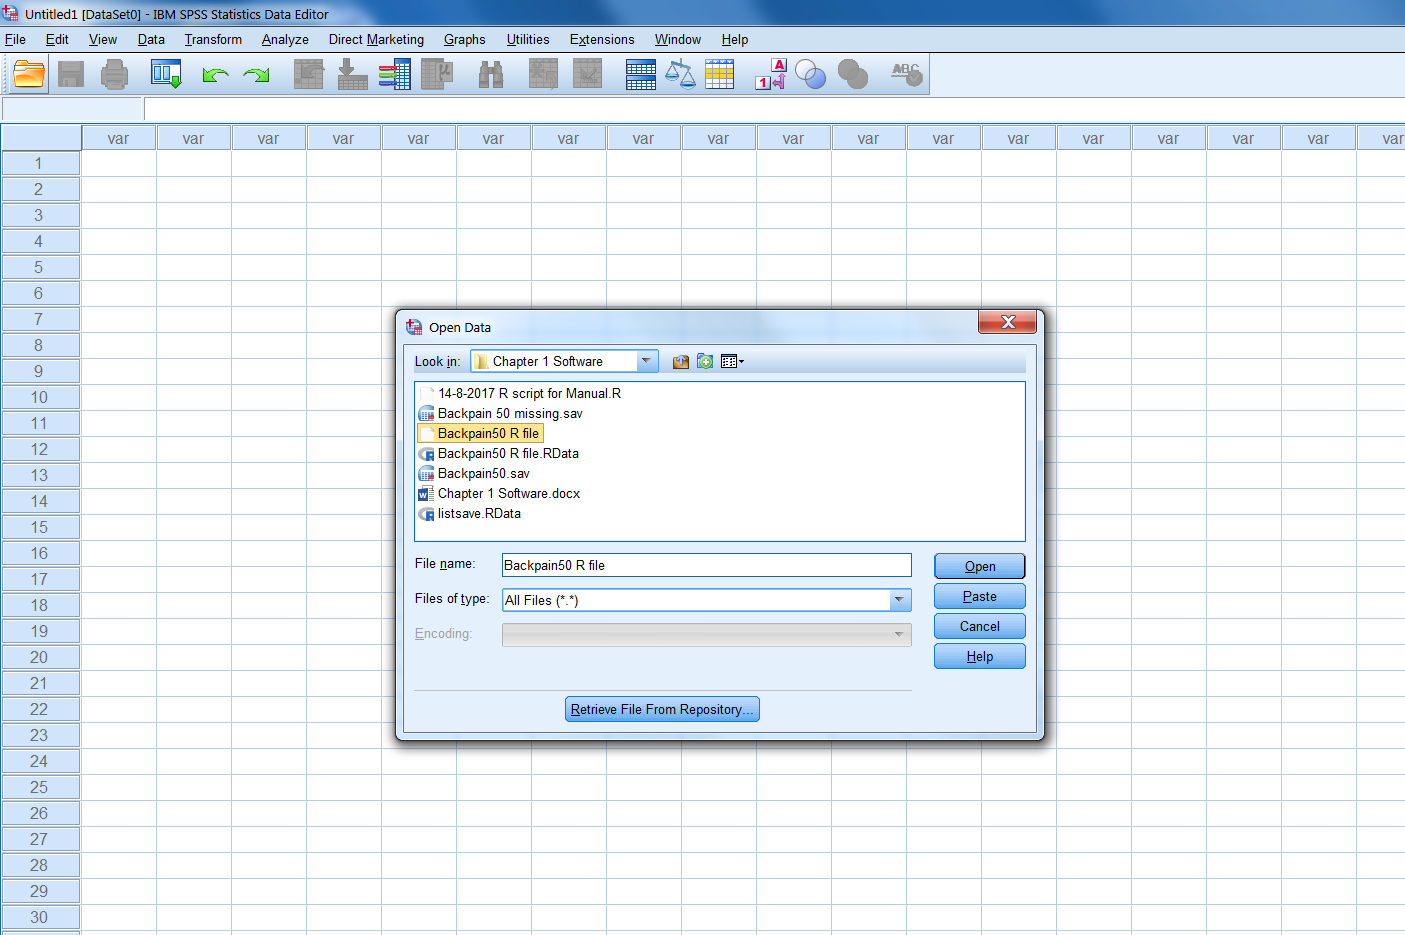
\includegraphics[width=0.9\linewidth]{images/fig1.18} 

}

\caption{Choosing the dataset to import in SPSS}\label{fig:fig18}
\end{figure}

Then click Open (wait a couple of seconds) and click on next. You will
see the following window that is part of the Text Import Wizard
procedure in SPSS (Figure 1.19):

\begin{figure}

{\centering 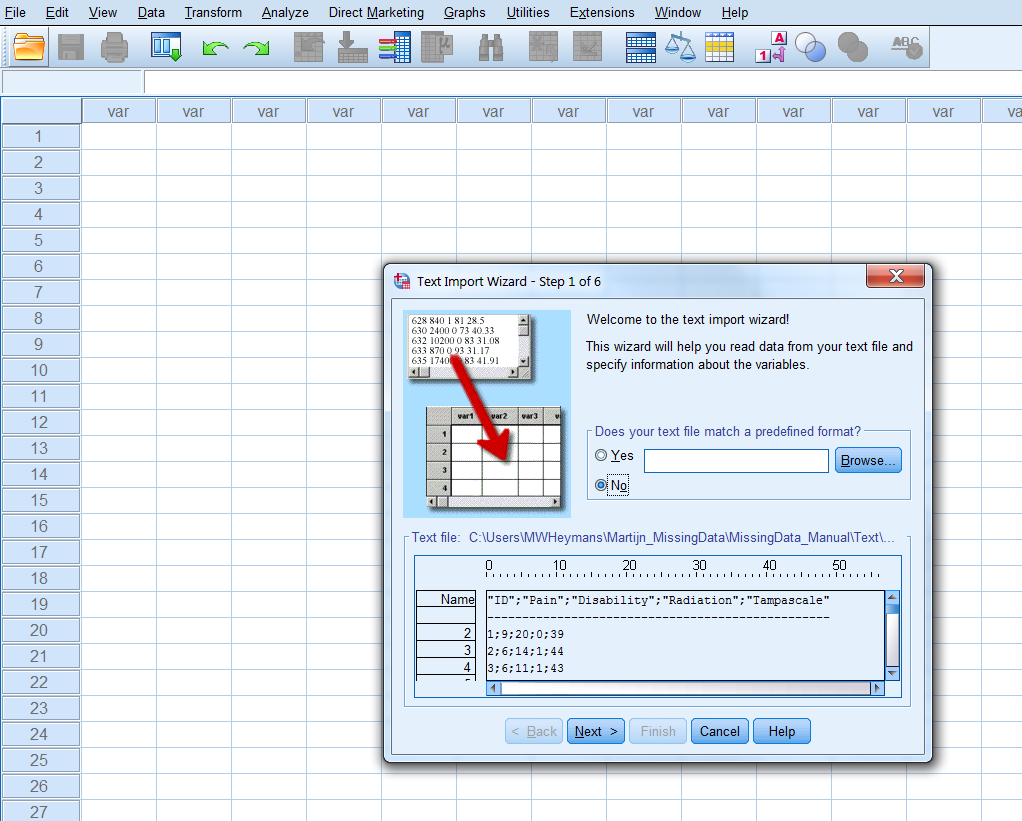
\includegraphics[width=0.9\linewidth]{images/fig1.19} 

}

\caption{Step 1 of the Text Import Wizard}\label{fig:fig19}
\end{figure}

Then click the ``Next \textgreater{}'' button 5 times, passing by the
following windows:

Step 2 of 6 (Figure 1.20): To change how variables are arranged: here
delimited To include variable names included at the top of the file:
here Yes. To set the decimal symbol: here a comma.

\begin{figure}

{\centering 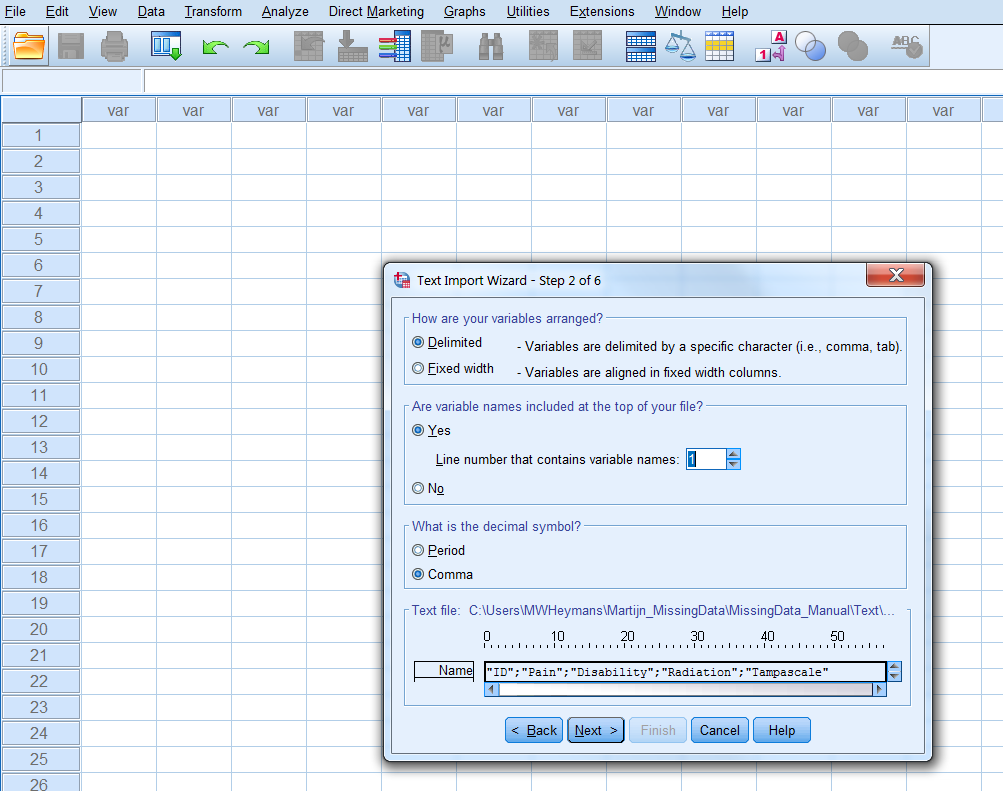
\includegraphics[width=0.9\linewidth]{images/fig1.20} 

}

\caption{Step 2 of the Text Import Wizard}\label{fig:fig20}
\end{figure}

Step 3 of 6 (Figure 1.21):

On which line number begins the first case: here 2 How cases are
represented: Each line is a case. How many cases you want to import:
here all cases.

\begin{figure}

{\centering 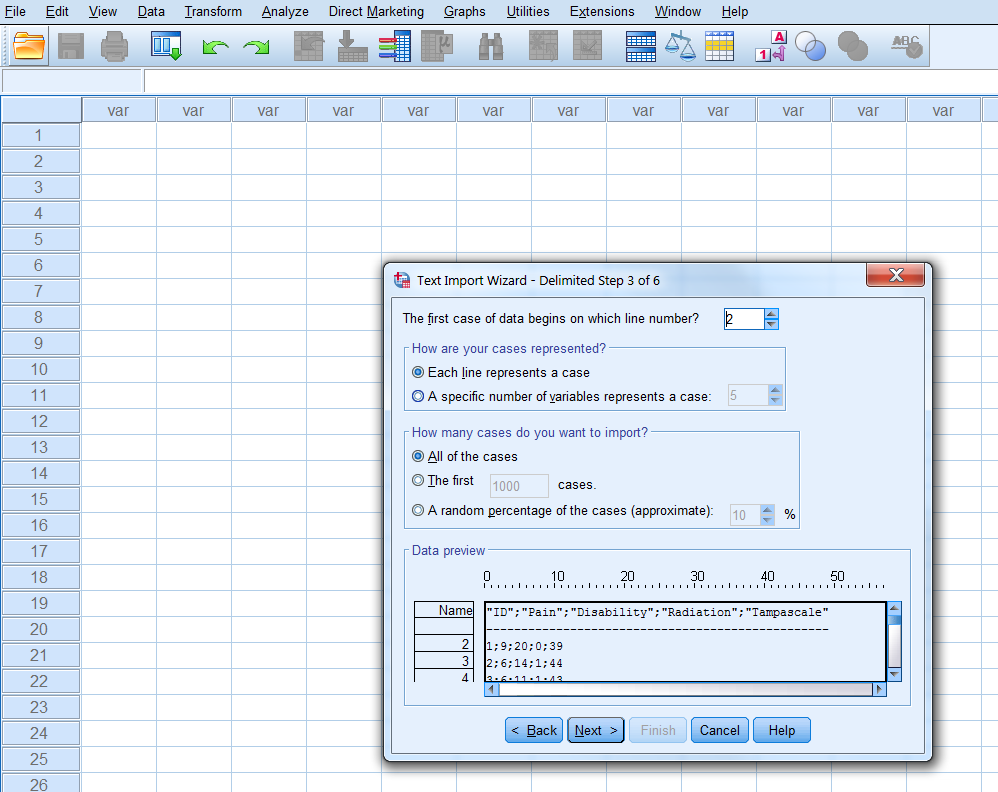
\includegraphics[width=0.9\linewidth]{images/fig1.21} 

}

\caption{Step 3 of the Text Import Wizard}\label{fig:fig21}
\end{figure}

Step 4 of 6 (Figure 1.22): The delimiters that appear between variables;
here the Semicolon. The text qualifier: here Double quote. Remove
trailing spaces from string values: skip.

\begin{figure}

{\centering 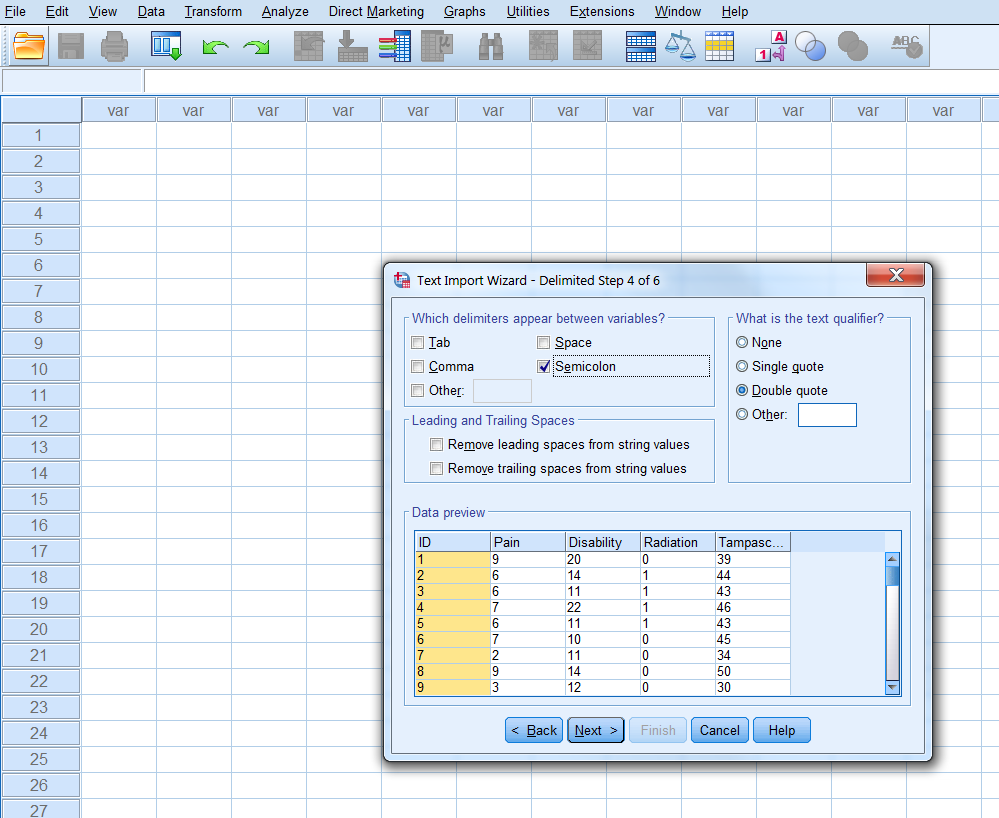
\includegraphics[width=0.9\linewidth]{images/fig1.22} 

}

\caption{Step 4 of the Text Import Wizard}\label{fig:fig22}
\end{figure}

Step 5 of 6 (Figure 1.23): Here you can overwrite the Data format of the
variable (you can also change that in the Variable View window, when the
data has been read in).

\begin{figure}

{\centering 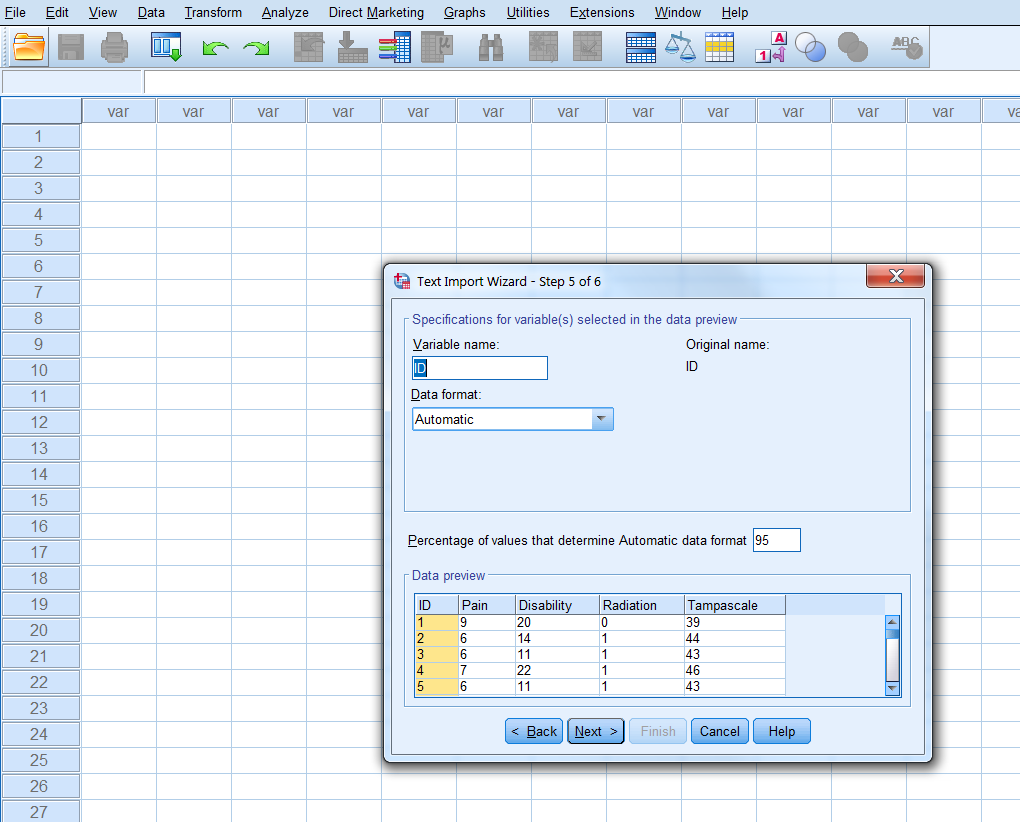
\includegraphics[width=0.9\linewidth]{images/fig1.23} 

}

\caption{Step 5 of the Text Import Wizard}\label{fig:fig23}
\end{figure}

Step 6 of 6: This step allows you to save your specifications of the
previous steps into a separate file (Figure 1.24).

\begin{figure}

{\centering 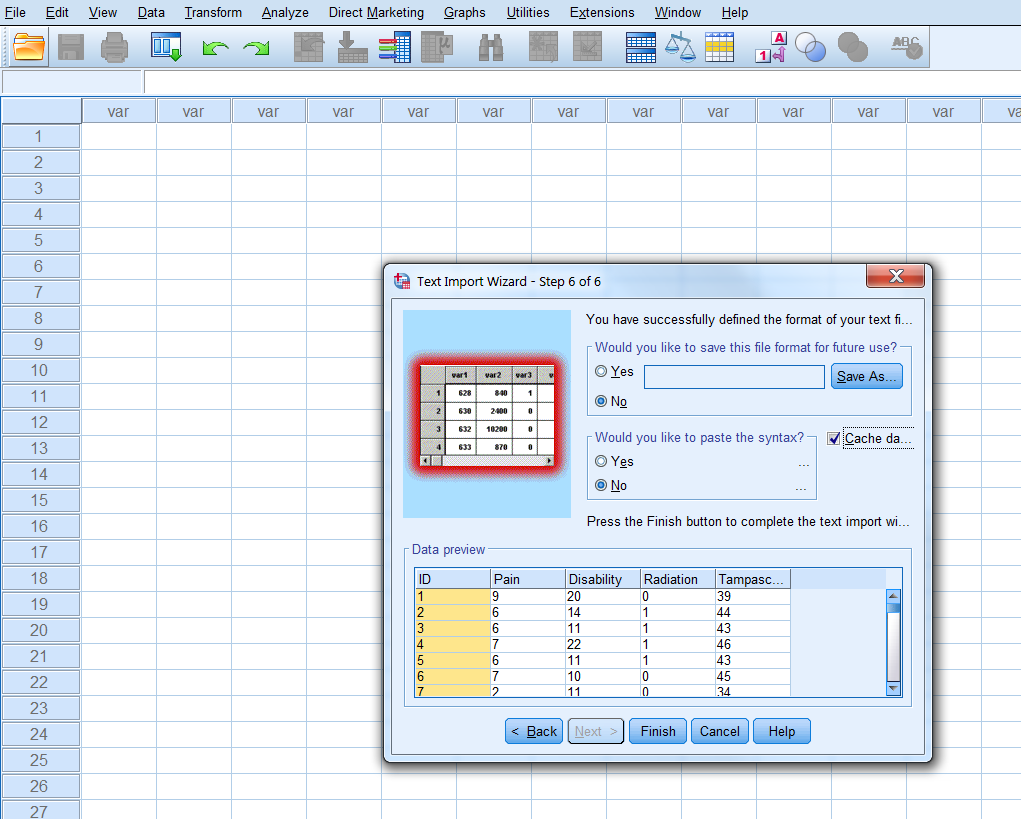
\includegraphics[width=0.9\linewidth]{images/fig1.24} 

}

\caption{Step 6 of the Text Import Wizard}\label{fig:fig24}
\end{figure}

Then click finish and the data will be read in, into a new SPSS file. In
that file you can of course change all kind of variable and data
settings in the Variable View Window.

You can also skip step 2 to 5 by clicking the Finish button twice when
you are at step 1. Than you use all default settings, which is most of
the times a good option.

\subsection{Installing R Packages}\label{installing-r-packages}

When R is installed on your computer also a folder called library is
created. This folder contains packages that are part of the basic
installation. A package is a collection of different functions written
in the R language. Besides packages that are part of the basic
installation of R there are also packages that are not part of the basic
installation but are written by others, i.e.~the add-on packages.
Packages can be downloaded from the CRAN website
(\url{https://cran.r-project.org/}). Currently, there are thousands of
user-written packages available on the CRAN website.

Before you can use a specific package that is not part of the basic
installation, you have to install it in your R library. In this manual
we will use the mice package to do all kind of imputation procedures,
such as multiple imputation. mice is not part of the basic installation
so we have to install it first. There are several procedures in RStudio
to install a package. One way is to use the install.packages function in
the Console window as follows:

The mice package will be automatically downloaded from the CRAN website.

Another way is to use the window on the right site below and go to the
Packages tab. When you click ``Install'' a new window is opened. Than
you can type ``mice'' on the blank line under ``Packages (separate
multiple with space or comma):'' (Figure 1.25a and b).

\begin{figure}

{\centering 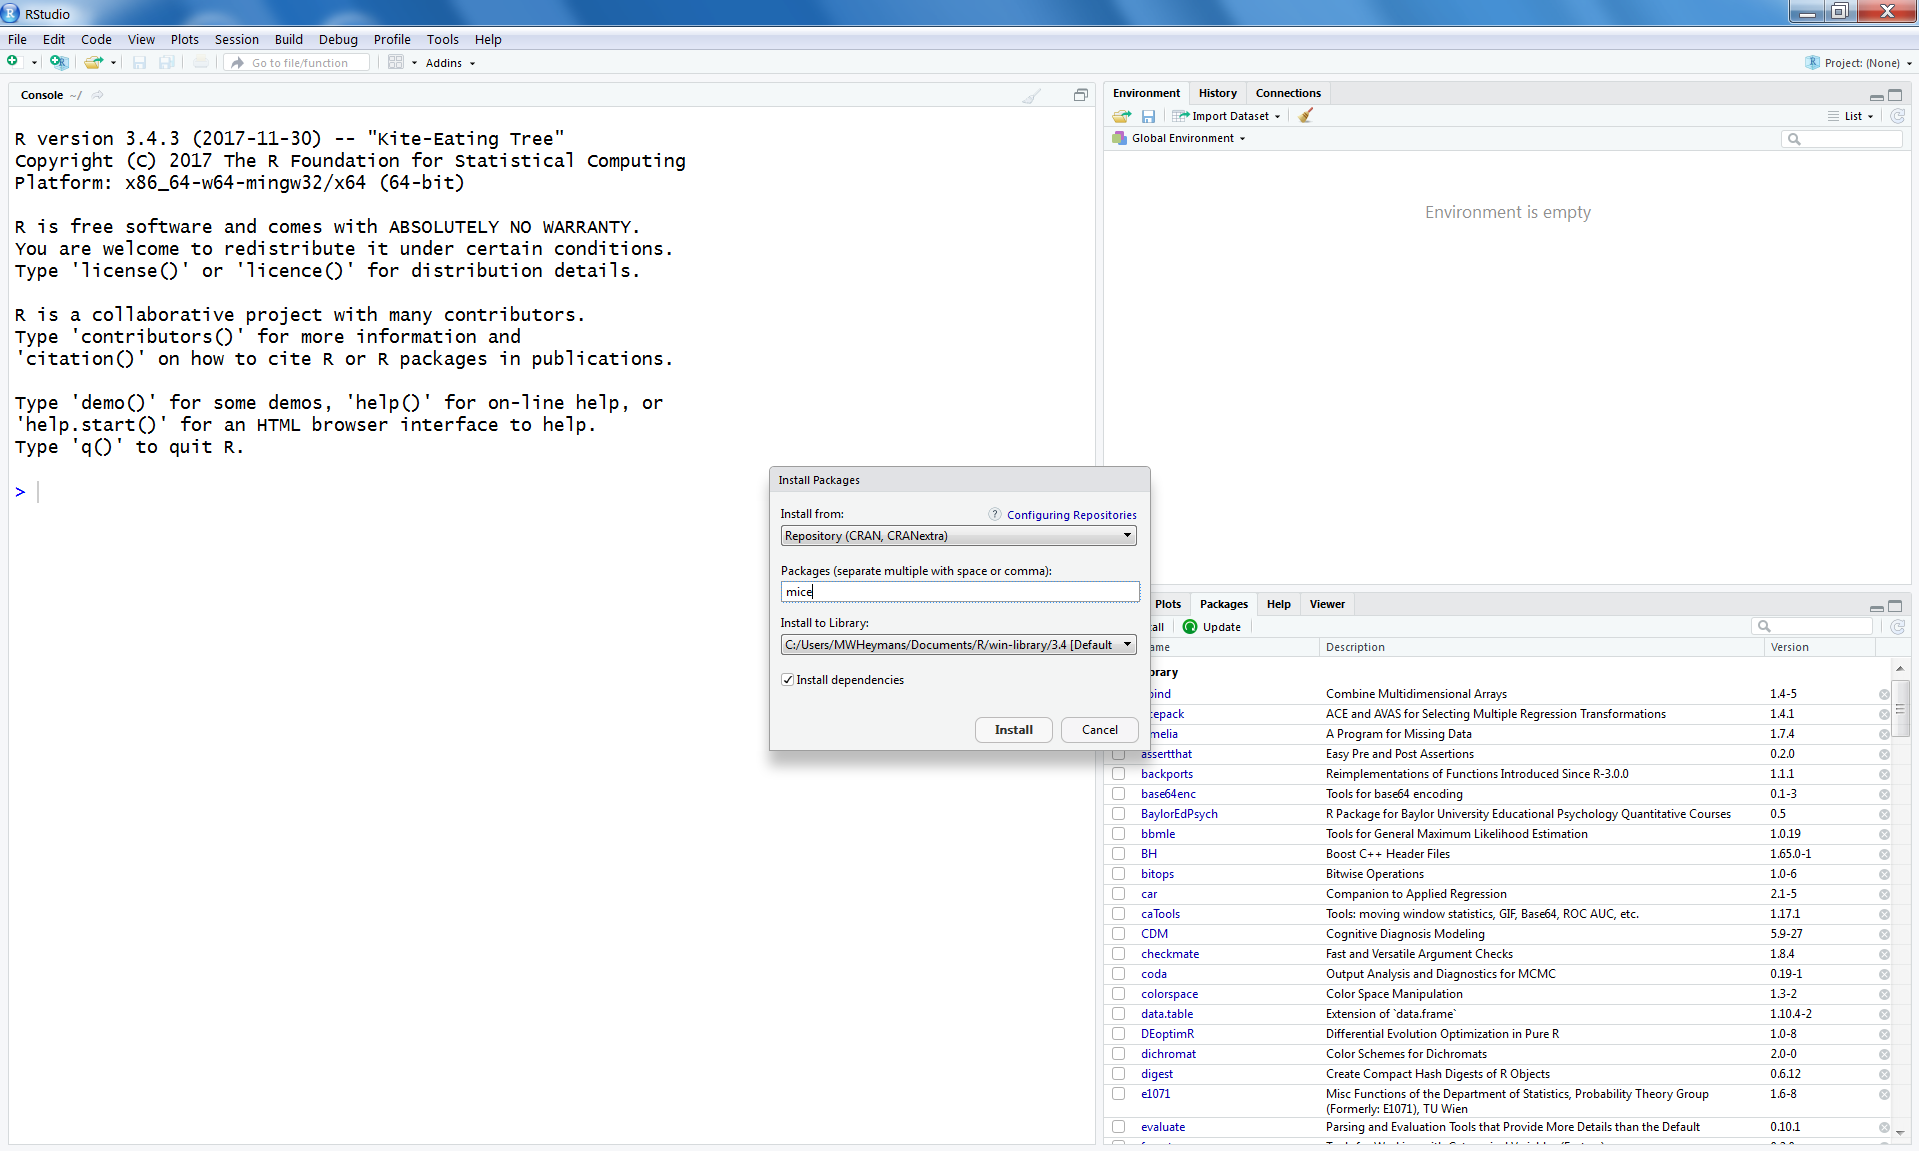
\includegraphics[width=0.9\linewidth]{images/fig1.25a} 

}

\caption{Install packages Window in RStudio to install packages from the CRAN website}\label{fig:fig25a}
\end{figure}

\begin{figure}

{\centering 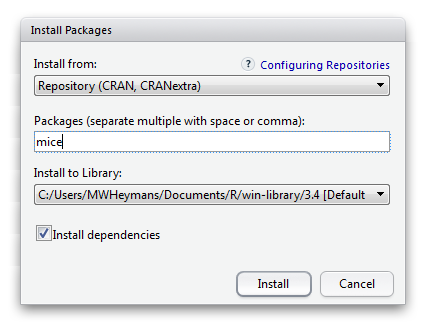
\includegraphics[width=0.9\linewidth]{images/fig1.25b} 

}

\caption{Enlarged Install packages Window in RStudio to install packages from the CRAN website}\label{fig:fig25b}
\end{figure}

After you have clicked on ``Install'' the package will be downloaded
from the CRAN website automatically and will be listed in the Package
list named ``User Library''.

Another way is to go to the CRAN website and download the package as a
zip file in a directory on your computer, for example your working
directory or in your library. Again use the window on the right site
below and go to the Packages tab. When you choose Install a new window
is opened. Now under ``Install from:'' choose for ``Package Archive File
(.zip; .tar.gz)'' (Figure 1.26a and 1.26b). Than you can browse to the
zip file and install the package.

\begin{figure}

{\centering 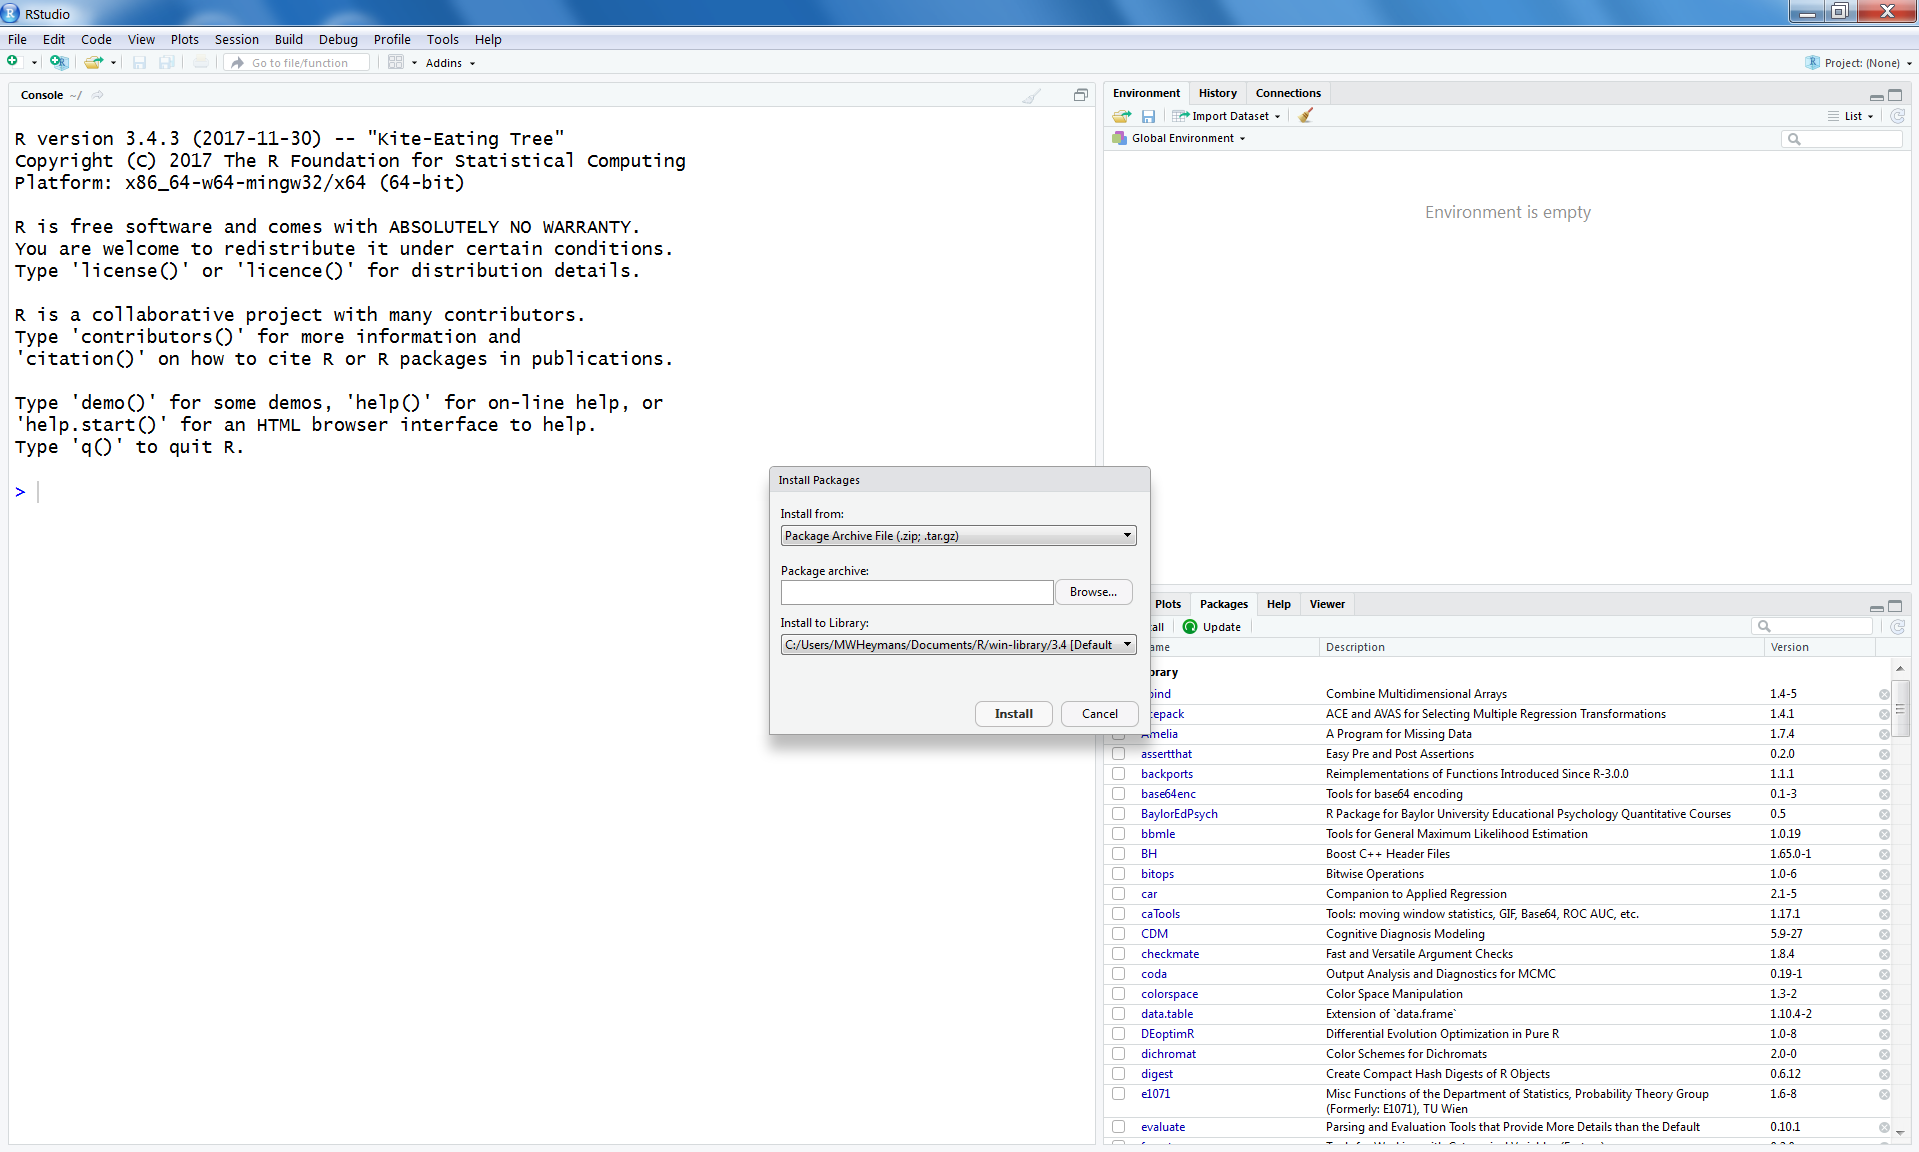
\includegraphics[width=0.9\linewidth]{images/fig1.26a} 

}

\caption{Install packages Window in RStudio to install packages from zip files}\label{fig:fig26a}
\end{figure}

\begin{figure}

{\centering 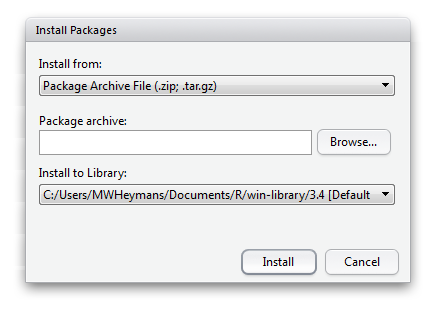
\includegraphics[width=0.9\linewidth]{images/fig1.26b} 

}

\caption{Enlarged Install packages Window in RStudio to install packages from zip files}\label{fig:fig26b}
\end{figure}

\subsection{Loading R Packages}\label{loading-r-packages}

Once an add-on (user written) R package has been installed it has to be
loaded to get access to all functions that are part of that package. To
load a library, you can use the function library() or require(). R code
1.43 shows an example of loading the mice package.

The require() function is used in the same way. You have to load add-on
packages each time you start a new R session.

\subsection{Updating R Packages}\label{updating-r-packages}

To keep the add-on packages up to date you can use the update.packages()
function in R. R code 1.44 presents an example.

R will ask you if you want to update each package. If you type ``y'' in
the Console window, R will update the package.

In RStudio updating packages can be done in the Package tab as well. You
can click on the Update button. A new window will open that contains a
list of all packages that need to be updated. Subsequently you can
select the packages you want to update.

\subsection{Useful Missing data Packages and
links}\label{useful-missing-data-packages-and-links}

The main package that we will use in this manual is mice which stand for
Multivariate Imputation by Chained Equations (MICE) (Van Buuren, 2009).

Other packages that are related to MICE are miceadds and micemd:
miceadds: this package contains some additional multiple imputation
functions (Robitzsch et al., 2017). See for more information:
\href{https://cran.r-project.org/web/packages/miceadds/index.html}{linked
phrase}

micemd: this package contains additional functions for the mice package
to perform multiple imputation in two-level (Multilevel) data (Audigier
\& Resche-Rigon, 2017). See for more information:
\href{https://cran.r-project.org/web/packages/micemd/index.html}{linked
phrase}

mi: provides functions for data manipulation, imputing missing values in
an approximate Bayesian framework, diagnostics of the models used to
generate the imputations, confidence-building mechanisms to validate
some of the assumptions of the imputation algorithm, and functions to
analyze multiply imputed data sets (Gelman et al., 2015). See for more
information:
\href{https://cran.r-project.org/web/packages/mi/index.html}{linked
phrase}

MItools: small package to perform analyses and combine results from
multiple-imputation datasets (Lumley, 2015). See for more information:
\href{https://cran.r-project.org/web/packages/mitools/index.html}{linked
phrase}

norm: this package is for the Analysis of multivariate normal datasets
with missing values. It contains the mi.inference function. This
function combines estimates and standard errors to produce a single
inference. Uses the technique described by Rubin (1987), which are
called the Rubin's Rules (RR) (Novo, 2015). See for more information:
\href{https://cran.r-project.org/web/packages/norm/index.html}{linked
phrase}

vim (visualization and imputation of missing values): This package
includes tools for the visualization of missing and/or imputed values.
In addition, the quality of imputation can be visually explored using
various univariate, bivariate, multiple and multivariate plot methods
(Templ et al., 2017). See for more information:
\href{https://cran.r-project.org/web/packages/mi/index.html}{linked
phrase}

BaylorEdPsych: R Package for Baylor University Educational Psychology
Quantitative Courses. This package included Little's MCAR test
(Beaujean, 2015). See for more information:
\href{https://cran.r-project.org/web/packages/BaylorEdPsych/index.html}{linked
phrase}

MKmisc: Contains several functions for statistical data analysis;
e.g.~for sample size and power calculations, computation of confidence
intervals, and generation of similarity matrices. This package contains
the mi.t.test function for pooling t-tests after multiple imputation
(Kohl, 2016). See for more information:
\href{https://cran.r-project.org/web/packages/MKmisc/index.html}{linked
phrase}

mvnmle: This package estimates the maximum likelihood estimate of the
mean vector and variance-covariance matrix for multivariate normal data
with missing values. This package is needed for the mlest function this
is used for Little's MCAR test in Cahpter 2. See for more information:
\href{https://cran.r-project.org/web/packages/mvnmle/index.html}{linked
phrase}

\chapter{Missing Data Evaluation}\label{missing-data-evaluation}

Before you decide what to do with your missing data it is important to
consider the reasons and probable causes of your missing data problem.
With that information you can compose an analysis plan to deal with the
missing data in your dataset. In this Chapter, you will learn how to
explore and evaluate your missing data in SPSS and R and why it is
important to think about the missing data mechanism. This knowledge is
important for the method you choose to handle the missing data problem.

\section{Definition of Missing Data}\label{definition-of-missing-data}

\subsection{Defining Missing Data in
SPSS}\label{defining-missing-data-in-spss}

Missing data in SPSS can be defined in two ways, as a system missing or
user missing value. System missing data is missing data that is not
present in the dataset and can be recognized by an empty cell (or dot).
User missing data is data that is coded as missing value in the dataset
by the user for some specific kind of reason. As an example we use a
small dataset with 50 Backpain patients consisting of males (coded as 1)
and females (coded as 0) patients (Figure 2.1). The female patients in
this dataset have been pregnant and the Gestational Age (GA) variable,
contains the duration of their pregnancy in weeks.

\begin{figure}

{\centering 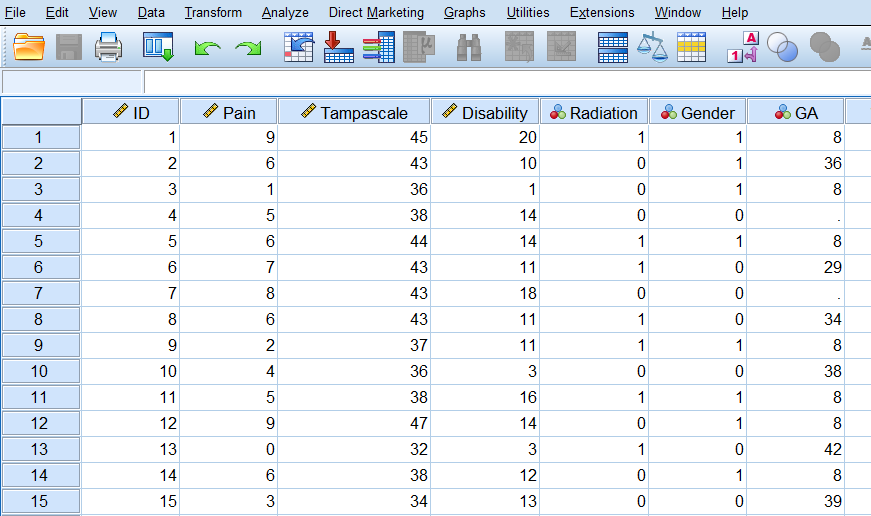
\includegraphics[width=0.9\linewidth]{images/fig2.1} 

}

\caption{SPSS dataset containing variables with system and user missing data}\label{fig:fig27}
\end{figure}

The Variable GA in the dataset consists of different values, like real
values for GA as 36 and 29, the value 8 and empty cells. The value 8 is
specified by us to exclude males from further analysis that include the
GA variable. This is a user missing value, that was indicated because
males cannot be pregnant. The system missing values are recognizable by
the empty cells (or dots) in the dataset, and these indicate the missing
GA values for women who did not report their GA. It makes no difference
if we code the missing values as a system or user missing value in SPSS,
because both kinds of missing values are recognized as missing values by
SPSS and will be excluded from further analyses.

\subsection{Missing data in R}\label{missing-data-in-r}

In R the missing values are denoted by NA which means ``Not Available''.
If we open the same dataset as above in R we get the following result.

\begin{Shaded}
\begin{Highlighting}[]
\KeywordTok{library}\NormalTok{(haven)}
\NormalTok{dataset <-}\StringTok{ }\KeywordTok{read_sav}\NormalTok{(}\StringTok{"data/CH2 example.sav"}\NormalTok{)}
\KeywordTok{head}\NormalTok{(dataset,}\DecValTok{10}\NormalTok{)}
\end{Highlighting}
\end{Shaded}

\begin{verbatim}
## # A tibble: 10 x 7
##       ID  Pain Tampascale Disability Radiation Gender    GA
##    <dbl> <dbl>      <dbl>      <dbl>     <dbl>  <dbl> <dbl>
##  1     1     9         45         20         1      1     8
##  2     2     6         43         10         0      1    36
##  3     3     1         36          1         0      1     8
##  4     4     5         38         14         0      0    NA
##  5     5     6         44         14         1      1     8
##  6     6     7         43         11         1      0    29
##  7     7     8         43         18         0      0    NA
##  8     8     6         43         11         1      0    34
##  9     9     2         37         11         1      1     8
## 10    10     4         36          3         0      0    38
\end{verbatim}

The Variable Gestational Age (GA) contains the values for GA (e.g.~36,
29, etc.), the value 8 for males and the NA's. In R the value 8 will be
treated as a real value, so we have to recode that value to NA by using
the following code.

\begin{Shaded}
\begin{Highlighting}[]
\NormalTok{dataset}\OperatorTok{$}\NormalTok{GA[dataset}\OperatorTok{$}\NormalTok{GA}\OperatorTok{==}\DecValTok{8}\NormalTok{] <-}\StringTok{ }\OtherTok{NA}
\KeywordTok{head}\NormalTok{(dataset,}\DecValTok{10}\NormalTok{)}
\end{Highlighting}
\end{Shaded}

\begin{verbatim}
## # A tibble: 10 x 7
##       ID  Pain Tampascale Disability Radiation Gender    GA
##    <dbl> <dbl>      <dbl>      <dbl>     <dbl>  <dbl> <dbl>
##  1     1     9         45         20         1      1    NA
##  2     2     6         43         10         0      1    36
##  3     3     1         36          1         0      1    NA
##  4     4     5         38         14         0      0    NA
##  5     5     6         44         14         1      1    NA
##  6     6     7         43         11         1      0    29
##  7     7     8         43         18         0      0    NA
##  8     8     6         43         11         1      0    34
##  9     9     2         37         11         1      1    NA
## 10    10     4         36          3         0      0    38
\end{verbatim}

The \texttt{NA} values will be recognized as missing values. For most
functions in R the handling of \texttt{NA} values has to be defined. For
example, the following code to obtain the mean of Gestational Age
results in an \texttt{NA} because the handling of missing data is not
defined.

\begin{Shaded}
\begin{Highlighting}[]
\KeywordTok{mean}\NormalTok{(dataset}\OperatorTok{$}\NormalTok{GA)}
\end{Highlighting}
\end{Shaded}

\begin{verbatim}
## [1] NA
\end{verbatim}

To obtain the mean of the observed data the following code has to be
used:

\begin{Shaded}
\begin{Highlighting}[]
\KeywordTok{mean}\NormalTok{(dataset}\OperatorTok{$}\NormalTok{GA, }\DataTypeTok{na.rm=}\OtherTok{TRUE}\NormalTok{)}
\end{Highlighting}
\end{Shaded}

\begin{verbatim}
## [1] 35.09524
\end{verbatim}

The \texttt{na.rm=TRUE} statement in the mean-function, indicates that
values that are NA need to be removed before the analysis can be
executed. Another NA handling procedure that is used in functions is
called na.action with as options \texttt{na.fail}, \texttt{na.omit},
\texttt{NULL} (no action) and \texttt{na.exclude}. For more information
about na.action options you can type the following code in the R console
\texttt{?na.action}.

\section{Missing data Patterns}\label{missing-data-patterns}

To get an idea about the complexity of the missing data problem in your
dataset and information about the location of the missing values, the
missing data pattern can be evaluated. Historically, the missing data
pattern was important as a starting point to choose the missing data
handling method (Little and Rubin, 2002). Currently, the missing data
pattern is less important because the most advanced (missing) data
analysis methods as multiple imputation can handle almost any missing
data pattern. We will discuss some frequently seen missing data
patterns, which are graphically displayed in Figure 2.2.

\begin{figure}

{\centering 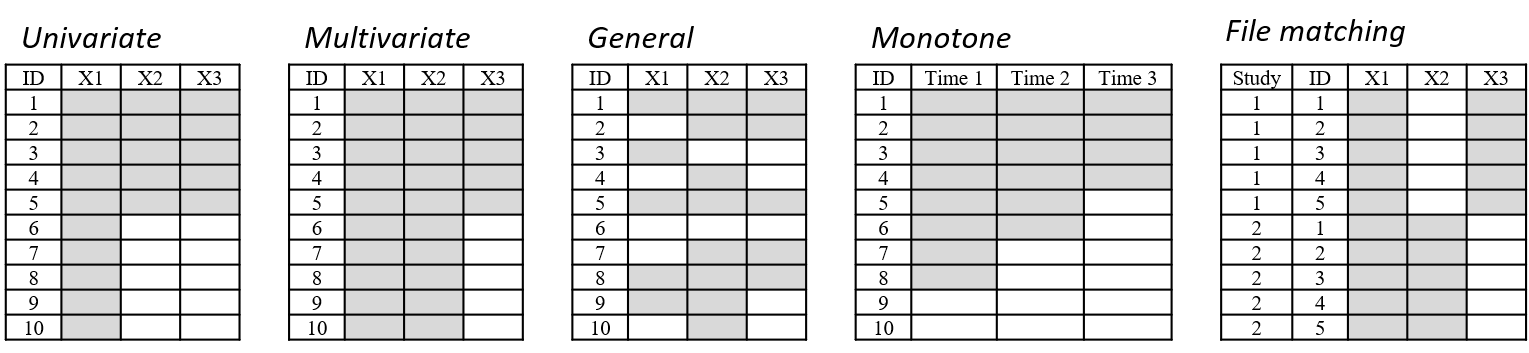
\includegraphics[width=0.9\linewidth]{images/fig2.2} 

}

\caption{Missing data patterns (ID means person identification number, X1 to X3 represent variables, Time 1 to 3 means that data is measured at 3 time points over time, Study means study number). The white cells represent the missing data}\label{fig:fig28}
\end{figure}

A univariate missing data pattern is a pattern with missing values in
only one variable (Figure 2.2a). An example of such a pattern is when
the independent variables are completely observed, but the outcome
variable is not, or when a selection of subjects refuse to fill in a
specific question such as their income level. Figure 2.2b and Figure
2.2c present examples of multivariate missing data patterns, where
multiple variables contain missing values. Figure 2.2b shows an example
where subjects miss values of the same two variables and Figure 2.2c
shows a more general pattern where different subject miss different
variable scores. A monotone pattern of missing data may occur in a
longitudinal study with data repeatedly assessed over time, and subjects
``drop-out'' of the study (Figure 2.2d). An example could be an elderly
study where persons become too frail to participate or just because
persons do not want to attend the study anymore because they are not
interested to fill in several questionnaires. A pattern called File
Matching can be observed when data from several studies is merged for an
individual participant data analysis and variables are not assessed in
all studies (Figure 2.2e). In our example, one variable is observed in
both studies (X1), but X2 and is only observed in study 1 and X3 in
study 2.

\subsection{Missing data patterns in
SPSS}\label{missing-data-patterns-in-spss}

\begin{quote}
To evaluate the missing data pattern, we can make use of the options
under the Missing Value Analysis (MVA) procedure in SPSS (IBM, 2016). We
use as an example a dataset that contains information of 150 Back pain
patients and 9 study variables. The variables are Pain (continuous),
Tampa scale (continuous), Radiation in the leg (dichotomous), Disability
(continuous), Body Weight (continuous), Body Length (continuous), Age
(continuous), Smoking (dichotomous), Gender (dichotomous). Only the
variables Gender and Age are completely observed.
\end{quote}

\begin{quote}
To access the MVA function in the SPSS menu choose: Analyze
-\textgreater{} Missing Value Analysis\ldots{} A new window will open
that is called ``Missing Value Analysis'' (Figure 2.3)
\end{quote}

\begin{figure}

{\centering 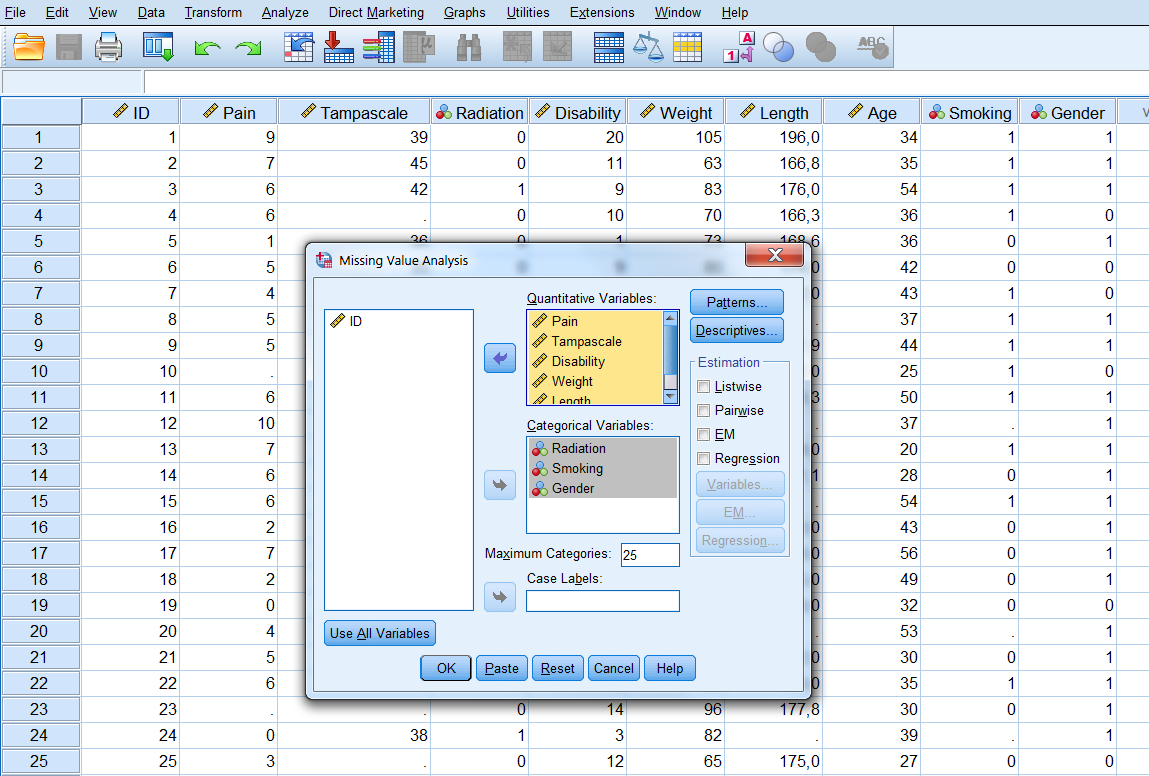
\includegraphics[width=0.9\linewidth]{images/fig2.3} 

}

\caption{The Missing Value Analysis menu}\label{fig:fig29}
\end{figure}

\begin{quote}
From this menu we first transfer all variables of interest in the
correct Quantitative and Categorical variables window and then choose
for the Patterns option. From the Patterns menu choose for the options
``Tabulated cases, grouped by missing value patterns'' and ``sort
variables by missing value pattern''. To obtain the full list of all
patterns that occur in the data, set the ``Omit patterns with less than
1\% of cases at 0\%, then click on continue and OK. This will produce
the output table that is displayed in Tables 2.1a and 2.1b.
\end{quote}

\begin{figure}

{\centering 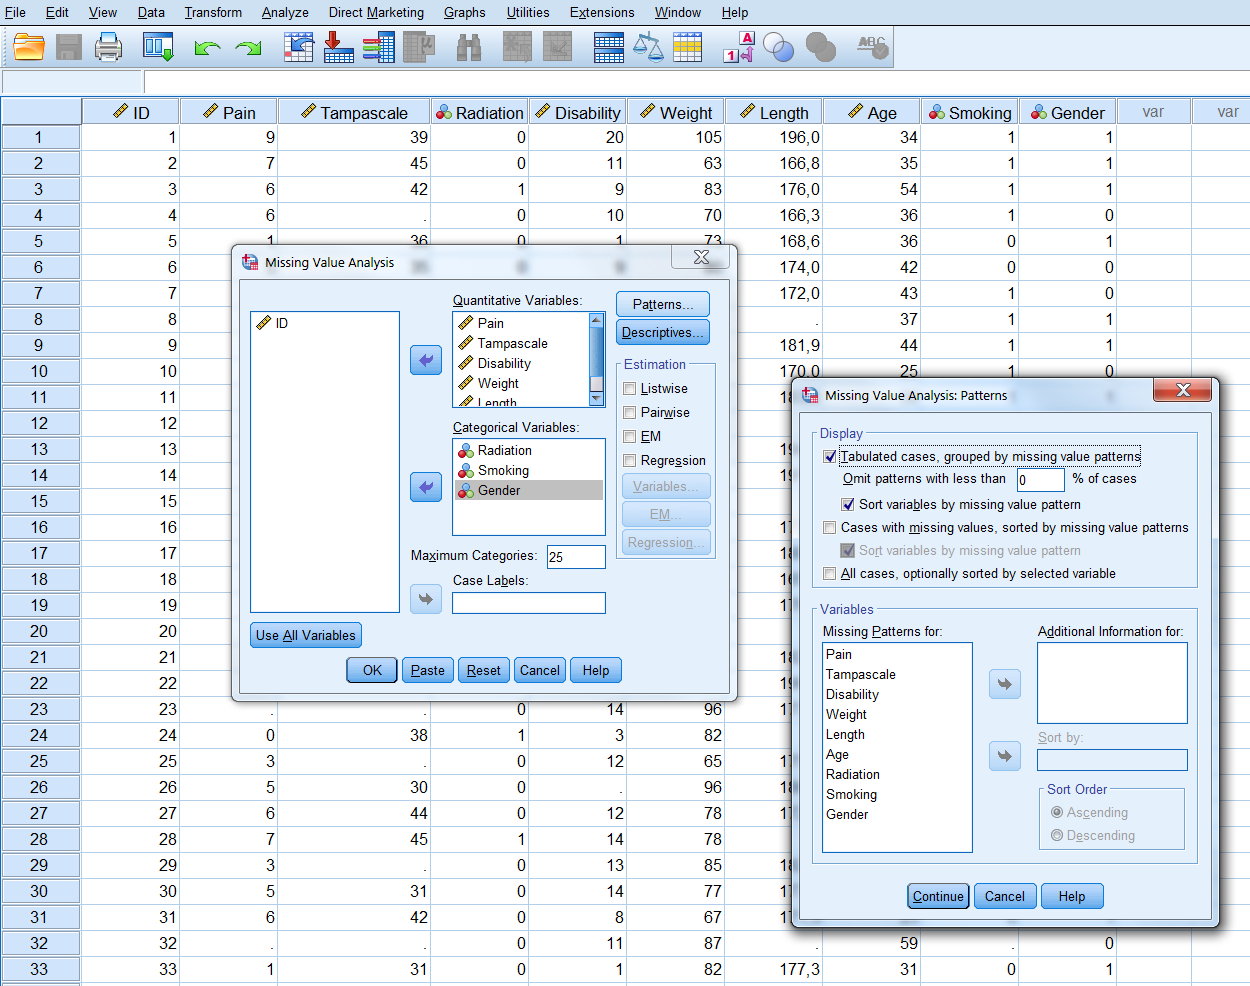
\includegraphics[width=0.9\linewidth]{images/fig2.4} 

}

\caption{The Patterns menu}\label{fig:fig30}
\end{figure}

As default procedure univariate statistics are presented including
output information about the number and percentages of missing data and
other descriptive statistics for each variable. Information about the
missing data patterns is provided in the Tabulated patterns table. On
the left column of that table, named ``Number of Cases'', the number of
cases are presented with that specific missing data pattern. In our
example, there are 75 cases in total without any missing values and 13
cases with a missing value in only the Tampa scale variable (see row 1
and 2 of Table 2.1). In the right column of that table named ``Complete
if\ldots{}'', the total number of subjects is presented if the variables
that contain missing data in that pattern are not used in the analysis.
Those variables are marked with the ``X'' symbol. For example, 88
subjects will be included in the analysis when the variable Tampa scale
is not used in the analysis, those are the 75 subjects that have
completely observed data on top of the 13 subjects with missing data in
the Tampa scale variable only.

\begin{figure}

{\centering 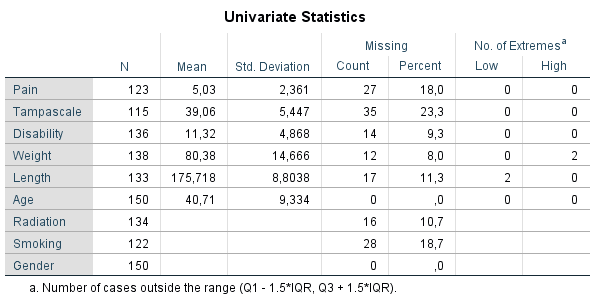
\includegraphics[width=0.9\linewidth]{images/tab2.1a} 

}

\caption{Descriptive missing data statistics and the missing data patterns.}\label{fig:tab1}
\end{figure}\begin{figure}

{\centering 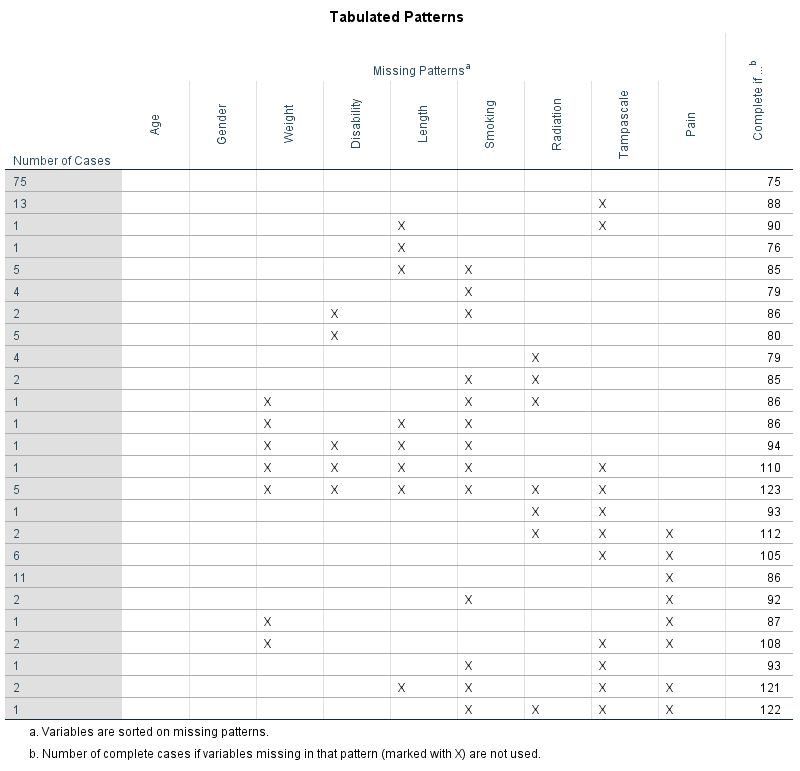
\includegraphics[width=0.9\linewidth]{images/tab2.1b} 

}

\caption{Descriptive missing data statistics and the missing data patterns.}\label{fig:tab1}
\end{figure}

\begin{quote}
Another way to obtain information about the missing data patterns is via
the Multiple Imputation option. To access this option, choose: Analyze
-\textgreater{} Multiple Imputation -\textgreater{} Analyze
Patterns\ldots{} A new window ``Analyze Patterns'' will open (Figure
2.5).
\end{quote}

\begin{figure}

{\centering \includegraphics[width=0.9\linewidth]{images/fit2.5} 

}

\caption{Analyse Patterns menu.}\label{fig:fig31}
\end{figure}

\begin{quote}
Now transfer all variables that have to be analyzed for their missing
values to the window ``Analyze Across Variables''. We choose for the
following output options in that window: Summary of missing values
(displays missing data information in pie charts, Patterns of missing
values (displays tabulated patterns of missing values) and Variables
with the highest frequency of missing values (displays a table of
analysis variables sorted by percent of missing values in decreasing
order). To get the full list of all patterns set the ``Minimum
percentage missing for variable to be displayed'' at 0. You can also
adjust the maximum number of variables displayed. This procedure will
generate the following output.
\end{quote}

\begin{figure}

{\centering \includegraphics[width=0.9\linewidth]{images/fit2.6a} 

}

\caption{Output as a result of the Analyze Patterns menu under Multiple Imputation.}\label{fig:fig32}
\end{figure}\begin{figure}

{\centering \includegraphics[width=0.9\linewidth]{images/fit2.6b} 

}

\caption{Output as a result of the Analyze Patterns menu under Multiple Imputation.}\label{fig:fig32}
\end{figure}\begin{figure}

{\centering \includegraphics[width=0.9\linewidth]{images/fit2.6c} 

}

\caption{Output as a result of the Analyze Patterns menu under Multiple Imputation.}\label{fig:fig32}
\end{figure}\begin{figure}

{\centering \includegraphics[width=0.9\linewidth]{images/fit2.6d} 

}

\caption{Output as a result of the Analyze Patterns menu under Multiple Imputation.}\label{fig:fig32}
\end{figure}

\subsection{Missing data patterns in
R}\label{missing-data-patterns-in-r}

To generate the missing data patterns in R we can make use of the mice
and \texttt{VIM} packages. We start with the \texttt{mice} package. That
package contains the \texttt{md.pattern} function that can generate the
missing data pattern.

\begin{Shaded}
\begin{Highlighting}[]
\KeywordTok{library}\NormalTok{(mice)}
\KeywordTok{md.pattern}\NormalTok{(dataset)}
\end{Highlighting}
\end{Shaded}

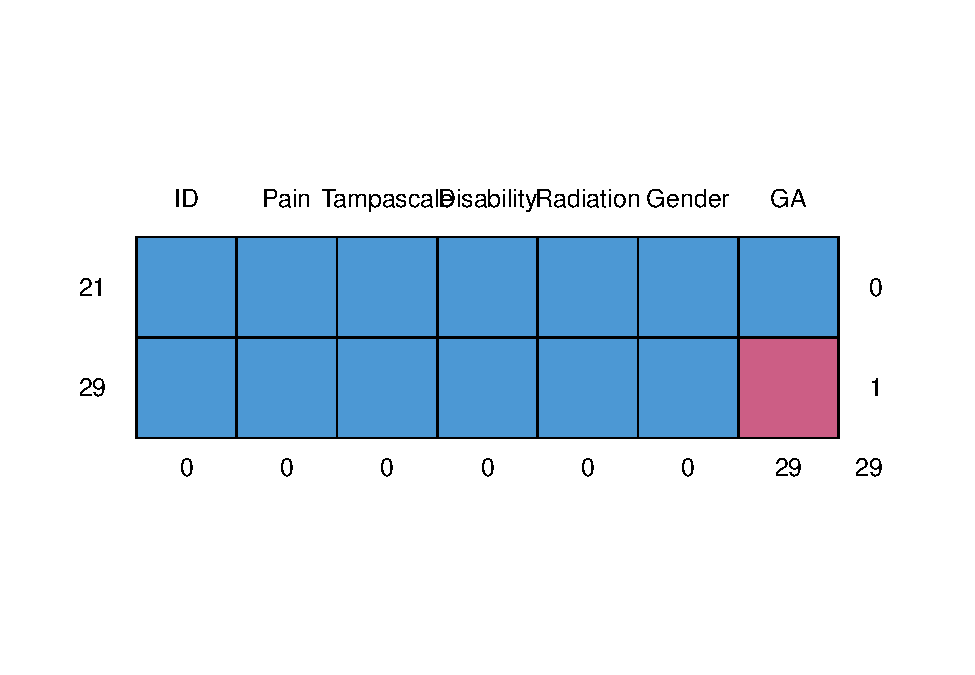
\includegraphics{Book_MI_files/figure-latex/unnamed-chunk-55-1.pdf}

\begin{verbatim}
##    ID Pain Tampascale Disability Radiation Gender GA   
## 21  1    1          1          1         1      1  1  0
## 29  1    1          1          1         1      1  0  1
##     0    0          0          0         0      0 29 29
\end{verbatim}

The first row contains the variable names. Each other row represents a
missing data pattern. The 1's in each row indicate that the variable is
complete and the 0's indicate that the variable in that pattern contains
missing values. The first column on the left (without a column name)
shows the number of cases with a specific pattern and the column on the
right shows the number of variables that is incomplete in that pattern.
The last row shows the total number of missing values for each variable.

To obtain a visual impression of the missing data patterns in R we use
the \texttt{VIM} package. That package contains the function
\texttt{aggr} As a result of using this function, the univariate
proportion of missing data is given in the Console window together with
two graphs.

\begin{Shaded}
\begin{Highlighting}[]
\KeywordTok{library}\NormalTok{(VIM)}
\KeywordTok{aggr}\NormalTok{(dataset, }\DataTypeTok{col=}\KeywordTok{c}\NormalTok{(}\StringTok{'white'}\NormalTok{,}\StringTok{'red'}\NormalTok{), }\DataTypeTok{numbers=}\OtherTok{TRUE}\NormalTok{, }\DataTypeTok{sortVars=}\OtherTok{TRUE}\NormalTok{, }\DataTypeTok{cex.axis=}\NormalTok{.}\DecValTok{7}\NormalTok{, }\DataTypeTok{gap=}\DecValTok{3}\NormalTok{, }\DataTypeTok{ylab=}\KeywordTok{c}\NormalTok{(}\StringTok{"Percentage of missing data"}\NormalTok{,}\StringTok{"Missing Data Pattern"}\NormalTok{))}
\end{Highlighting}
\end{Shaded}

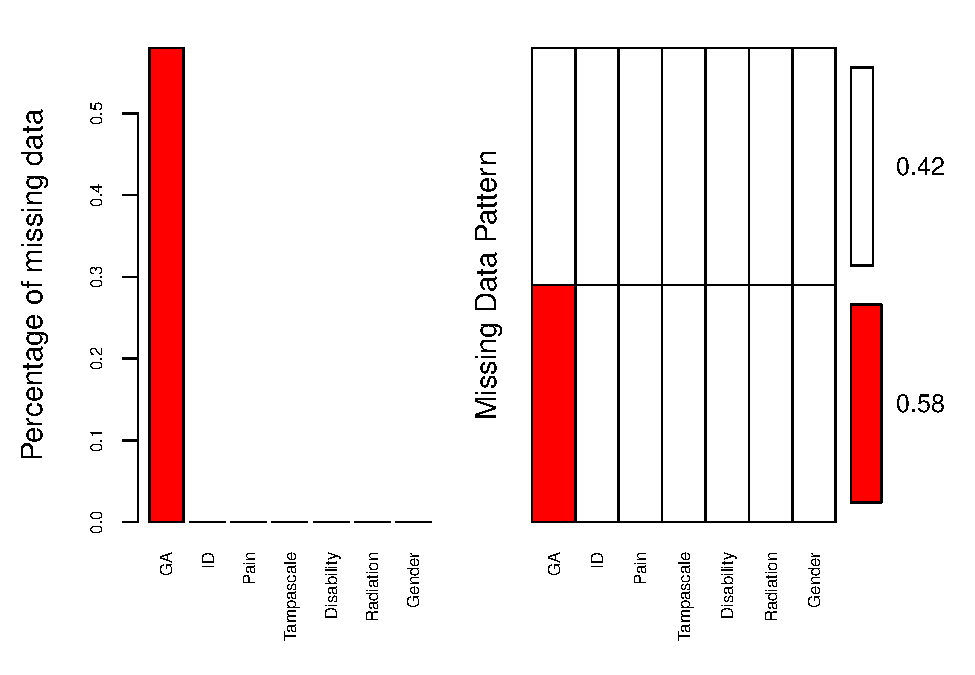
\includegraphics{Book_MI_files/figure-latex/unnamed-chunk-56-1.pdf}

\begin{verbatim}
## 
##  Variables sorted by number of missings: 
##    Variable Count
##          GA  0.58
##          ID  0.00
##        Pain  0.00
##  Tampascale  0.00
##  Disability  0.00
##   Radiation  0.00
##      Gender  0.00
\end{verbatim}

A histogram is displayed with the univariate percentage of missing
values in each variable, which is also shown as output in the Console
window and the patterns of missing data are also displayed. At the right
side of Figure 2.8 the proportion of patterns is presented. The variable
names are shown at the bottom of the figures. The red cells in the
Missing data patterns figure indicate that those variables contain
missing values. We see that 0.500 or 50\% of the patterns do not contain
missing values in any of the variables. Of the total patterns, 8.67\% of
the patterns have missing values in only the Tampa scale variable.

\section{2.3 Missing data Mechanisms}\label{missing-data-mechanisms}

By evaluating the missing data patterns, we can get insight in the
location of the missing data. With respect to the missing data mechanism
we are interested in the underlying reasons for the missing values and
the relationships between variables with and without missing data. In
general, we can say that missing values are either random or non-random.
Random missing values may occur because subjects accidentally do not
answer some questions or information of an entire subject is
accidentally not assessed. For example, a study subject has to fill out
some questionnaire instruments, gets distracted and misses a question
accidently or a questionnaire gets lost in the mail. Non-random missing
values may occur because subjects purposefully do not answer questions.
For example, subjects may be reluctant to answer questions about
sensitive topics like income, past crimes or sexual history. Rubin
introduced in 1976 a typology for missing data that makes a distinction
between random and non-random missing data situations, which are
abbreviated as MCAR, MAR and MNAR. These types of missing data are still
used as the basic missing data mechanisms. The key idea behind Rubin's
missing data mechanisms is that the probability of missing data in a
variable may or may not be related to the values of other measured
variables in the dataset. This means that we assume that there is some
kind of probability model for the missing data. With probability we
loosely mean the likelihood of a missing value to occur, i.e.~if a
variable has a lot of missing data, the probability of missing data in
that variable is high. This probability (i.e.~likelihood) can be related
to other measured or not-measured variables. For example, when mostly
older people have missing values, the probability for missing data is
related to age. Moreover, the missing data mechanisms also assume a
certain relationship (or correlation) between observed and variables
with missing values in the dataset. The extend of the relation between
observed variables and the probability of missing data, distinguishes
the three missing data mechanisms. In essence the missing data
mechanisms describe relationships between variables that may or may not
be causal, because in most missing data situations we never know the
real reason why data is missing. We will discuss the missing data
mechanisms in more detail below. As an example, we will use a study on
Low Back Pain (LBP). It is known that people with LBP may develop a fear
of movement (which is assessed by the Tampa scale) due to their pain in
the back. The idea is that these people believe that some underlying
serious problem causes their back pain and in order to prevent for more
damage they are afraid to move their back and experience a high fear of
movement.

\subsection{2.3.1 Missing Completely At
Random}\label{missing-completely-at-random}

Data are Missing Completely At Random (MCAR) when the probability that a
value is missing, is unrelated to the value of other observed (or
unobserved) variables, and unrelated to values of the missing data
variable itself. We will discuss what is means by using the LBP study as
an example. If LBP patients had to come to a research center to fill in
the Tampa scale (fear of movement) questionnaire and supply other
information for the study and some patients were not able to come
because they were ill that day due to the flu. In case of MCAR, there is
no relationship between having the flu and scores on the Tampa scale or
other study-related variables. This is realistic because there is no
evidence that patients with the flu, fear their back problem more, or
that the odds of having the flu is related to the study. For that
reason, we can assume that the missing data are MCAR. In other words,
the probability of missing data is not related to the values of the
Tampa scale variable. Another example is when respondents accidentally
skip questions in a questionnaire. Than the observed values of that
questionnaire are just a random sample of the entire dataset. An MCAR
missing data situation for the Tampa scale variable is visualized in the
MCAR column in the figure below. Although in real live we actually do
not know the completely observed data, as an example (for educational
reasons), the MCAR column is a copy of the completely observed Tampa
scale variable, with some values removed. When we compare the MCAR data
with the complete Tampa scale variable scores, we can observe that in
the MCAR situation an equal number of lower and higher values of the
Tampa scale variable are missing (in total 4 Tampa scores are missing, 2
for lower and 2 for higher values,). Also, the missing data in the Tampa
scale do not seem to be related to another variable like pain; an equal
number of Tampa scale values is missing for patients with low pain
scores as well as for patients with higher pain scores. This means that
the (observed) probability of missing data in the Tampa scale variable
will be equally large for lower and higher values of the Tampa scale and
of other measured variables in the data (i.e.~pain).

\begin{figure}

{\centering 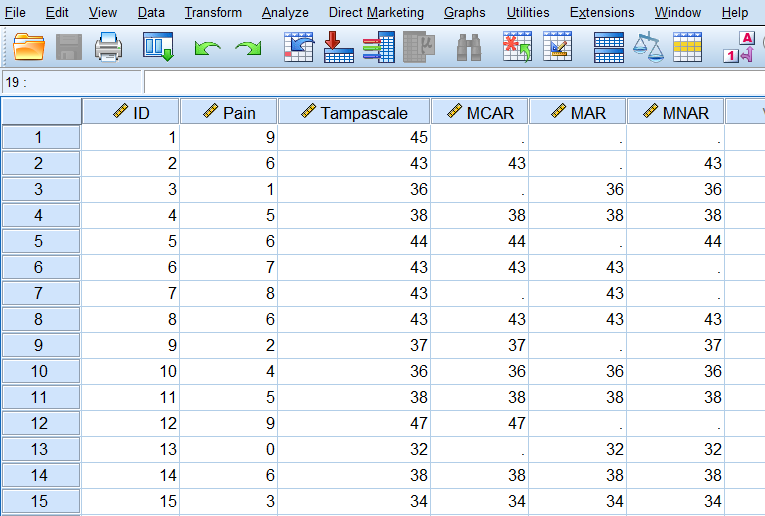
\includegraphics[width=0.9\linewidth]{images/fig2.7} 

}

\caption{Examples of MCAR, MAR and MNAR data.}\label{fig:fig33}
\end{figure}

This phenomenon for the Tampa scale variable in the LBP study is shown
in Table 2.2 below. This Table shows that the percentages (or observed
probabilities) of missing data are equally large for lower, middle and
higher values of the Tampa scale variable. These values are presented as
Percentile Groups of Tampa scale values with a range of 28-34, 35-37,
38-40, 41-44, 45-50 respectively. Over the whole range, the percentage
of missing data is around 25\% (equally large for different values and
(not shown) this is also the case for lower and higher values of other
variables e.g.~pain). In general, The MCAR mechanism does not lead to
parameter estimation problems as for example invalid mean or regression
coefficient estimates. However, excluding cases with MCAR data will
result in a smaller dataset for the analysis and thus larger standard
errors (i.e.~lower power).

\begin{figure}

{\centering 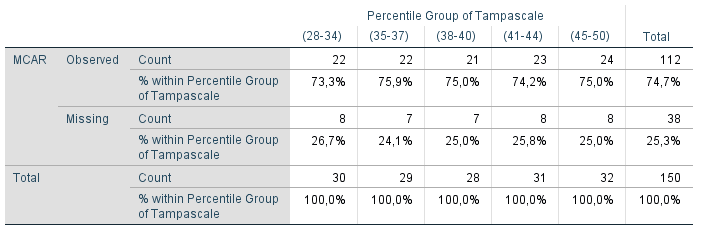
\includegraphics[width=0.9\linewidth]{images/tab2.2} 

}

\caption{MCAR missing data in the Tampa scale variable.}\label{fig:tab2}
\end{figure}

\subsection{Missing At Random}\label{missing-at-random}

The data are Missing At Random (MAR) when the probability that a value
for a variable is missing is related to other observed values in the
dataset but not to the variable itself. The reason of missing data may
lie outside the dataset but observed variables in the dataset capture
this by their associations. An example of MAR data is presented in the
MAR column of Figure 2.9 and in Table 2.3 below for 150 LBP patients. In
Figure 2.9 you can see in the MAR column that 4 Tampa scale scores are
missing for pain scores that are ≥ 6 and 1 for a pain score \textless{}
6, in other words the probability of missing data in the Tampa scale
scores is higher for higher pain scores. In other words, patients with
higher pain scores (≥ 6) have more missing values on the Tampa scale
variable than patients with lower pain scores (\textless{} 6). However,
within the category of pain scores with values ≥ 6, the Tampa scale
scores are MCAR, because within each category Tampa scale scores are
randomly missing for lower and higher values. In Table 2.3 the Tampa
scale data is split for at lower and higher pain score categories. It
can be observed that the means and standard deviations do not differ
between the observed and missing data for the Tampa scale variable.
Which is an indication that the Tampa scale data are MAR. (for
educational purposes we know the values of the missing values). A reason
could be that patients with higher Tampa scale scores were less likely
to show up at a next Tampa scale measurement because their back hurted
more. In a MAR missing data situation, missing values can be explained
by other (observed) variables, like for the Tampa scale and Pain
variable in the example above, due to the their (statistical)
relationship in the dataset. Further, within categories of the pain
variable (for low and high pain values) the Tampa scale scores are MCAR
(Raghunathan, 2016). However, it is not possible to test this
assumption, because for that you need information of the missing values
and that is impossible. In general, excluding MAR data leads to false
estimates of your statistical tests, like for example, regression
coefficients. A missing data method that works well with MAR data is
Multiple Imputation (Chapter 4).

\begin{figure}

{\centering 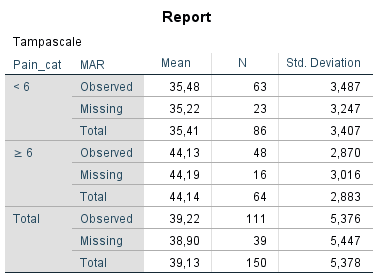
\includegraphics[width=0.9\linewidth]{images/tab2.3} 

}

\caption{MAR missing data in the Tampa scale variable.}\label{fig:tab34}
\end{figure}

\subsection{Missing Not At Random}\label{missing-not-at-random}

The data are MNAR when the probability of missing data in a variable is
related to the scores of that variable itself, e.g.~only high or low
scores are missing, and this missing data problem cannot be captured
anymore by other measured variables in the dataset because they are not
available in the dataset. In case of the LBP example, MNAR data occurs
when patients with the highest scores on the Tampa scale have missing
values. This is shown in the MNAR column of Figure 2.9. The MNAR column
shows that the values that are most frequently missing are the highest
Tampa scale scores, i.e.~for the patients that fear their back problems
most. A reason may be that these patients were so afraid to move (which
is assessed by the Tamp scale), that they were not able to visit an
assessment center. MNAR missing data can also occur indirectly through
the relationship of the variable with missing data with another variable
that is not available in the dataset. For example, it could also be that
patients that worry the most do not want to be confronted with questions
about their fear to move their back and therefore skip questions of the
Tampa scale. In case of a positive relationship between worriedness and
fear of movement, the highest values on the Tampa scale variable will be
missing for those patients that worry the most. If worriedness is not
measured in the dataset, the missing data in the Tampa scale variable
will be MNAR. The difference with MAR is that with MNAR, the missing
data problem cannot be handled by the observed variables in the dataset
or by using a technique as Multiple Imputation. However, as with MAR
data, MNAR data can also not be verified.

\subsection{The Missing Data
Indicator}\label{the-missing-data-indicator}

In the definitions of the missing data mechanisms in the previous
paragraphs we used the term probability several times, to indicate that
the relationship of variables with the probability of missingness in a
variable distinguishes the missing data mechanisms. The probability of
missing data can depend on other variables (MAR), on values of the
variables itself (MNAR) or not on other variables or values of the
variable itself (MCAR). Rubin (1987) proposed that variables with
missing data can be divided in a part that is observed and a part that
is missing. The observed and missing data can be coded by a 0 and 1
respectively. In case of the Tampa scale variable this means that the
observed data is coded by a 0 and a 1 is used for the Tampa scale values
that are missing. This dichotomous coding variable is called the missing
data indicator or R variable which means that the complete and missing
data are defined according to this variable. Figure 2.10 shows the R
indicator variable for the observed and missing data in the Tampa scale
variable. The R variable is now a single variable because there is
missing data in only the Tampa scale variable. When more variables
contain missing data, the R variable becomes a dataset of variables that
consist of 0´s and 1´s.

\begin{figure}

{\centering 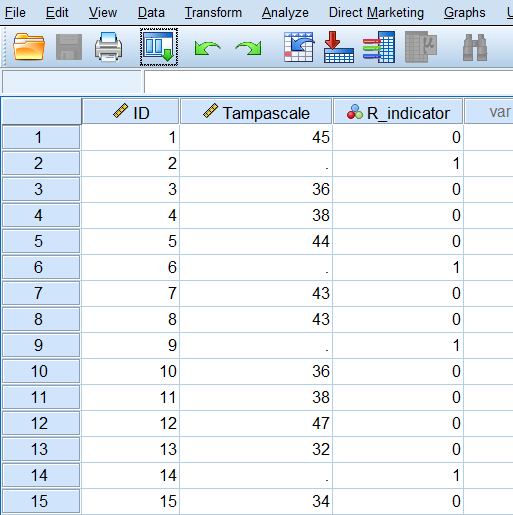
\includegraphics[width=0.9\linewidth]{images/fig2.8} 

}

\caption{The missing data in the Tampa scale variable coded according to the missing data indicator variable R.}\label{fig:fig34}
\end{figure}

Using the R indicator variable implies that missing values (or the
probability of missing values) can be described by a missing data model.
This missing data model may consist of variables that have a
relationship with the probability of missing data, in this case the R
indicator variable. A good example would be to use a logistic regression
model to describe the relationship of variables with the probability of
missing data in the Tampa scale variable. Graphically these models can
be visualized as in Figure 2.11. With logistic regression, which is in
essence a probability model, the relationship of a dichotomous outcome
variable (i.e.~the R missing data indicator variable) with other
variables can be described by using the models that are shown in Figure
2.12. In this Figure the missing data indicator variable R of the Tampa
scale variable that contain missing values is the outcome variable.

\begin{figure}

{\centering 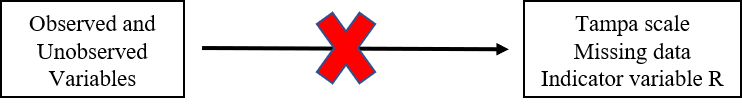
\includegraphics[width=0.9\linewidth]{images/fig2.9a} 

}

\caption{MCAR}\label{fig:fig35}
\end{figure}

There is no relationship between, how the data became missing (indicated
by R) and observed and unobserved variables.

\begin{figure}

{\centering 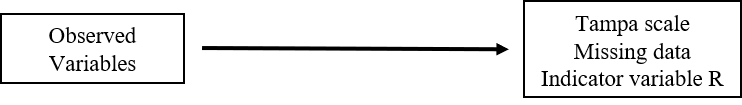
\includegraphics[width=0.9\linewidth]{images/fig2.9b} 

}

\caption{MAR}\label{fig:fig36}
\end{figure}

There is a relationship between, how the data became missing (indicated
by R) and observed variables.

\begin{figure}

{\centering 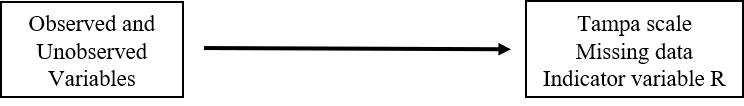
\includegraphics[width=0.9\linewidth]{images/fig2.9c} 

}

\caption{MNAR}\label{fig:fig37}
\end{figure}

There is a relationship between, how the data got missing (indicated by
R) and observed and unobserved variables.

The missing data mechanisms of Rubin can then be described by the
following logistic regression models:

MCAR: No variables in or outside the dataset explain the missingness in
the Tampa scale variable, the model would be empty:
\[LN(\frac{R_{Tampa=1}}{1-R_{Tampa=1}}) = \beta_0\]

MAR: Variables in the dataset, like Pain and Radiation in the Leg
explain the missingness in the Tampa scale variable and the model would
be:
\[LN(\frac{R_{Tampa=1}}{1-R_{Tampa=1}}) = \beta_0 + \beta_1 * Pain + \beta_2 * Radiation\]

MNAR: Missingness in the Tampa scale variable can be explained by
variables in the dataset and by the score on the Tampa scale itself:

\[LN(\frac{R_{Tampa=1}}{1-R_{Tampa=1}}) = \beta_0 + \beta_1 * Pain + \beta_2 * Radiation + \beta_3 * Tampa\]

From these models we observe that the missing data models can be defined
by other observed variables in the dataset and/or missing data (which we
do not observe). It should be noted however, that we can never be
completely sure about the reason why data are missing. The above
mentioned relationships are therefore statistical relationships from
descriptive models and not from causal models.

In summary, the MCAR assumption is mostly very strict and not realistic
in practice.The MAR assumption is more realistic and mostly assumed in
practice.The difference bewteen MAR and MNAR is that in MNAR the
probability of missingness is also related to the unobserved (missing)
data.

\subsection{The Role of Auxiliary
Variables}\label{the-role-of-auxiliary-variables}

Usually, the probability of missing data is related to other variables
and/or to the missing values itself (MAR or MNAR). Unfortunately, it is
not possible to distinguish between MAR and MNAR mechanisms, because the
missing values are unknown. Brand (Brand, 1999) describes in Chapter 2
of his dissertation two examples that demonstrate how an initially MNAR
missing data mechanism can change into MAR by including additional
variables that are related to the probability of missing data. In
practice, by including variables related to the probability of missing
data a MNAR mechanism can get closer to a MAR mechanism. Accordingly,
the MAR assumption can be made more plausible by including additional
information in the missing data handling method (Baraldi \& Enders,
2010). Therefore, it is advised, to include extra variables that have a
relationship with the missing data rate in other variables, i.e.~have a
relationship with the probability of missing data or that have a
relationship (correlated) with the variables that contain the missing
values (Collins, 2001, Curran, Bacchi, Schmitz, Molenberghs, \&
Sylvester, 1998). These variables are called auxiliary variables and are
included in the imputation procedure to generate valid imputations.
These variables may not be required for further data analyses. In
general, the MCAR assumption is unrealistic and does not hold in most
datasets. As a practical solution, many studies assume a MAR mechanism.
Mostly, this mechanism is realistic, however it is advised to evaluate
the plausibility of this assumption in analyses explained below.

\section{Missing Data evaluation}\label{missing-data-evaluation-1}

A useful data evaluation and data imputation method depends on the
underlying missing data mechanism that is assumed. We have seen in
Paragraph 2.3 that the difference between the MCAR and not MCAR
mechanisms depend on the relationship of the missing data with the
observed variables. If this relationship cannot be detected by the
observed data in the dataset we assume that the data is MCAR. If there
is some kind of relationship, the missing data may be MAR or MNAR. We
can never distinct between MAR or MNAR data, because for that we need
information about the missing values and we do not have that
information. Tests to distinguish the missing data assumptions are
therefore only aimed to accept or reject the MCAR missing data
assumption. The MCAR assumption is mostly a too strict assumption to use
in practice because there is commonly some kind of reason why persons do
not fill in ``working'' questions. Moreover, in practice we study and
measure outcome and independent variables that are related to each
other. This makes that the MAR assumption is the most accepted
``working'' missing data assumption in practice. There are two ways to
evaluate the missing data mechanism. First, it is important to think
about the most plausible substantive reasons for the data being missing.
Researchers mostly have some possible explanation about why data are
missing and this information is very important. For example, when during
web based data collection, the internet sometimes disconnects because of
malfunction at the address of the internet provider, data of a few
participants gets lost. When these malfunctions are coincidental, it can
be assumed that the missing data are MCAR. However, when cognitive
scores are assessed during this web based data collection and these are
mostly not filled out by people that have decreased cognitive functions,
the missing data can be assumed to be MNAR. There are statistical test
procedures that can be used to get an idea about the missing data
mechanism. In these statistical tests, the non-responders (i.e.,
participants with missing observations), can be compared to the
responders on several characteristics. By doing this, we can test
whether the missing data mechanism is likely to be MCAR or not-MCAR
(because we cannot distinguish between MAR and MNAR missing data). There
are several possibilities to compare the non-responders with the
responders groups, for example using t-tests, a logistic regression with
a missing data indicator as the outcome, or Little's MCAR test (Little,
1988). To discuss these tests, we will use the example data from the
previous chapter, where we have measured several variables in a group of
150 low back pain patients and some variables contain missing
observations. In the examples below we will assume a MAR missing data
mechanism for the variables Tampa scale and Disability. Researchers need
to be aware that the assumptions that underlie an independent t-test,
logistic regression, and Chi-square test apply to these missing data
mechanism procedures as well. This means that the data is assumed to be
normally distributed and that the tests depend on a decent sample size.

\subsection{Missing data Evaluation in
SPSS}\label{missing-data-evaluation-in-spss}

\subsubsection{Descriptive Statistics}\label{descriptive-statistics}

\begin{quote}
Descriptive information of variables can be obtained via the following
options of the Missing Value Analysis (MVA) module in the SPSS menu:
Analyze -\textgreater{} Missing Value Analysis\ldots{} than transfer all
variables in the correct Quantitative and Categorical variables window
and then clock Descriptives option -\textgreater{} Univariate
statistics.
\end{quote}

\begin{figure}

{\centering 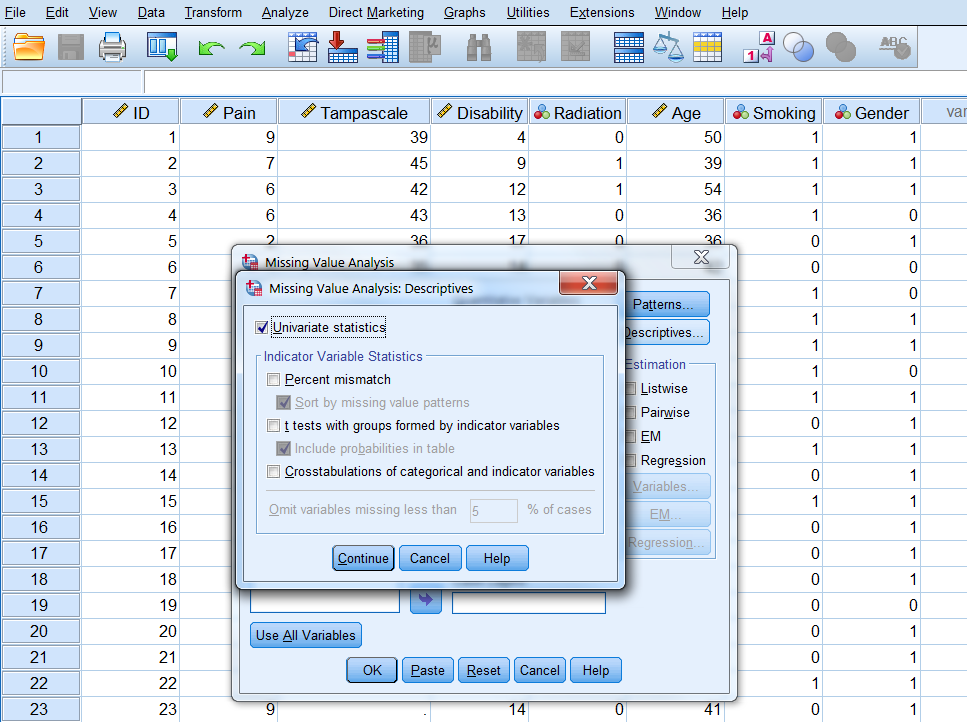
\includegraphics[width=0.9\linewidth]{images/fig2.10} 

}

\caption{Missing value Analysis menu in SPSS}\label{fig:fig38}
\end{figure}

\begin{figure}

{\centering 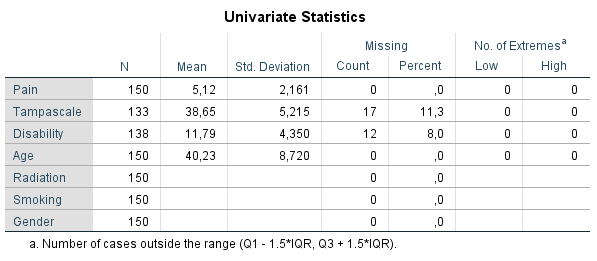
\includegraphics[width=0.9\linewidth]{images/tab2.4} 

}

\caption{Univariate descriptive statistics of variables with and without missing data.}\label{fig:tab4}
\end{figure}

Under the column N, the information of all cases in the dataset are
displayed, under the column Missing we get the number and percentage of
missing values in each variable and under the column No. of Extremes we
get information of cases that fall outside a range, which is specified
under the table. Further, for all continuous variables information about
the Mean and Standard deviation are displayed. No descriptive
information is given for categorical variables.

These descriptive information of variables with missing data gives us a
quick overview of the amount of missing data in each variable. However,
it does not provide us information about the relationship between
variables with complete and missing data and therefore does not give us
an idea about the potential missing data mechanism. Methods as T-tests,
regression or Little's MCAR test, that will be discussed in the next
section, can better be used for that purpose.

\subsubsection{T-test procedure}\label{t-test-procedure}

When we use the t-test procedure, SPSS first creates an indicator
variable, to distinguish the cases with missing values from the cases
with values that are present in each variable with missing values. Then,
group means are estimated and compared for other variables that are
complete with groups formed by the indicator variable, using Student's t
test. As a result, the t-statistic, degrees of freedom, counts of
missing and non-missing values, and means of the two groups are
displayed. You can also display any two-tailed probabilities associated
with the t statistic.

\begin{quote}
The t-test procedure can be found in the Missing Value Analysis window
under Descriptives. In that window choose for ``t-tests with groups
formed by indicator variables'' and ``include probabilities in table''
under the Indicator Variable Statistics options and then Click on
Continue -\textgreater{} OK.
\end{quote}

\begin{figure}

{\centering \includegraphics[width=0.9\linewidth]{images/fig2.11} 

}

\caption{The T-test procedure as part of the Missing Value Analysis menu}\label{fig:fig39}
\end{figure}

\begin{figure}

{\centering \includegraphics[width=0.9\linewidth]{images/tab2.5} 

}

\caption{Output table of the t-test procedure.}\label{fig:tab5}
\end{figure}

On the left side oft the output table the names of the variables with
missing values are presented which are the Tampa scale and Disability
variables. Of these variables, indicator variables are defined which are
used to compare group means of other variables, that can be tested for
significance using independent t-tests. The results of these t-tests are
given in the table according to the information in separate rows on the
left side with the t-value (t), degrees of freedom (df), P-value
(P(2-tail)), numbers of observed and missing cases (\# Present and \#
Missing) and means of observed and missing cases (Mean(Present) and
Mean(Missing)) presented. The variables for which the indicator groups
are compared, are listed in the columns of the table and are the Pain,
Tampa scale, Disability and Age variables. For the Tampa scale variable
that contain missing values, only the observed mean is presented,
because for the missing cases the values are missing! Notice that in the
row of the Tampa scale variable the means of the Disability variable can
still be compared between the observed and missing cases, because they
do not miss values for exactly the same cases. Table 2.5 shows that
patients that have observed values on the Tampa scale variable (row
Mean(Present)) differ significantly from patients with missing values on
the Tampa scale variable (row Mean(Missing)) on Pain (P(2-tail = 0.033)
and Disability (P(2-tail = 0.039). When we look at the means of the Pain
variable, we see that the mean of patients with missing values on the
Tampa scale variable is higher compared to the mean of patients with
observed scores. This means that there is a higher probability of
missing data on the Tampa scale variable for patients with higher pain
scores. If Tampa scale and Pain scores are correlated, the missing
values on the Tampa scale variable can also be explained by the Pain
score variable. This is also the case for the Age variable, but now the
t-test is not significant. For the Disability variable, it is the other
way around. We see more missing data on the Tampa scale variable for
lower Disability scores.

\begin{quote}
In the Missing Value Analysis window under the Indicator Variable
Statistics options you can also choose for ``Crosstabulations of
categorical and indicator variables''. In that case a separate table is
displayed for each categorical variable with missing values. For each
category of the variable, the frequency and percentages of non-missing
values for the other variables is displayed as well as the percentages
of each type of missing value. To reduce the size of the table, you can
omit statistics that are computed for only a small number of cases by
adjusting the option ``Omit variables missing less than \% of cases''.
\end{quote}

\subsubsection{Logistic Regression
Analysis}\label{logistic-regression-analysis}

The missing data mechanism can also be evaluated with a logistic
regression procedure (Ridout, Society, \& Diggle, 1991). In the logistic
regression analysis, we can evaluate if the probability of missing data
is related to other variables in the data. For this procedure, we first
generate an indicator variable that separates the subjects with missing
values from the participants with observed values. This indicator
variable is used as the dependent variable in a logistic regression
analysis. A backward regression can be used to determine the strongest
predictors of missing data. The output for the logistic regression with
the Tampa scale variable as the indicator outcome variable is presented
below:

\begin{figure}

{\centering \includegraphics[width=0.9\linewidth]{images/tab2.6} 

}

\caption{Logistic regression analysis with variable that contain missing data as the outcome variable.}\label{fig:tab6}
\end{figure}

We can observe that the variable Pain is significantly related to the
missing data indicator variable of the Tampa scale variable, which
indicates that the probability for missing data in the Tampa scale
variable can be explained by the Pain variable. The positive coefficient
of 0.315 indicates that the probability of missing data on the Tampa
scale variable is higher for higher Pain scores. The other variables do
not show a significant relationship with missing data on the Tampa scale
variable. This logistic regression analysis procedure can be repeated
for each variable with missing values in the dataset.

\subsubsection{Little's MCAR test in
SPSS}\label{littles-mcar-test-in-spss}

Another possibility is to use a test that was developed by Roderick
Little: Little's MCAR test. This test is based on differences between
the observed and estimated mean in each missing data pattern. This test
is developed for continuous data. In this procedure, the missing data in
the whole dataset is evaluated, because each missing data pattern is
included in the analysis. To conduct this test, you choose from the SPSS
menu:

\begin{quote}
Analyze -\textgreater{} Missing Value Analysis\ldots{}In the main
Missing Value Analysis dialog box, select the variable(s) for which you
want to estimate missing values (use only continuous variables) and
Select EM in the Estimation group and Click OK.
\end{quote}

\begin{figure}

{\centering \includegraphics[width=0.9\linewidth]{images/fig2.12} 

}

\caption{EM selection in the Missing Value Analysis menu.}\label{fig:fig40}
\end{figure}

\begin{figure}

{\centering \includegraphics[width=0.9\linewidth]{images/tab2.7a} 

}

\caption{Output tables with information of Little’s MCAR test.}\label{fig:tab7}
\end{figure}\begin{figure}

{\centering \includegraphics[width=0.9\linewidth]{images/tab2.7b} 

}

\caption{Output tables with information of Little’s MCAR test.}\label{fig:tab7}
\end{figure}\begin{figure}

{\centering \includegraphics[width=0.9\linewidth]{images/tab2.7c} 

}

\caption{Output tables with information of Little’s MCAR test.}\label{fig:tab7}
\end{figure}\begin{figure}

{\centering \includegraphics[width=0.9\linewidth]{images/tab2.7d} 

}

\caption{Output tables with information of Little’s MCAR test.}\label{fig:tab7}
\end{figure}\begin{figure}

{\centering \includegraphics[width=0.9\linewidth]{images/tab2.7e} 

}

\caption{Output tables with information of Little’s MCAR test.}\label{fig:tab7}
\end{figure}

\subsection{Missing data Evaluation in
R}\label{missing-data-evaluation-in-r}

\subsubsection{Little's MCAR test in R}\label{littles-mcar-test-in-r}

Little´s MCAR test is available in the \texttt{BaylorEdPsych} package
for R as the LittleMCAR function. To apply the test, we select only the
continuous variables. In the example blowe we use the dataset of 150 low
back pain patients with missing data in Genstatstional Age (GA). The
p-value for the test is not-siginificant, indicating that the missings
seem to be compeletely at random.

\begin{Shaded}
\begin{Highlighting}[]
\KeywordTok{library}\NormalTok{(BaylorEdPsych)}
\KeywordTok{LittleMCAR}\NormalTok{(dataset[,}\KeywordTok{c}\NormalTok{(}\StringTok{"Pain"}\NormalTok{, }\StringTok{"Tampascale"}\NormalTok{,}\StringTok{"Disability"}\NormalTok{, }\StringTok{"GA"}\NormalTok{)])}
\end{Highlighting}
\end{Shaded}

\begin{verbatim}
## this could take a while
\end{verbatim}

\begin{verbatim}
## $chi.square
## [1] 5.395246
## 
## $df
## [1] 3
## 
## $p.value
## [1] 0.14504
## 
## $missing.patterns
## [1] 2
## 
## $amount.missing
##                 Pain Tampascale Disability    GA
## Number Missing     0          0          0 29.00
## Percent Missing    0          0          0  0.58
## 
## $data
## $data$DataSet1
##    Pain Tampascale Disability GA
## 2     6         43         10 36
## 6     7         43         11 29
## 8     6         43         11 34
## 10    4         36          3 38
## 13    0         32          3 42
## 15    3         34         13 39
## 17    3         35         11 26
## 20    4         32          9 28
## 25    5         36          6 35
## 28    3         36          3 36
## 30    6         37         16 40
## 32    4         37          8 39
## 34    2         37          3 37
## 37    8         47          8 35
## 39    3         39          8 33
## 41    7         45         10 32
## 44    1         35          2 34
## 46    5         41         17 38
## 47    6         43         11 41
## 48    3         39          9 33
## 50    8         44         19 32
## 
## $data$DataSet2
##    Pain Tampascale Disability GA
## 1     9         45         20 NA
## 3     1         36          1 NA
## 4     5         38         14 NA
## 5     6         44         14 NA
## 7     8         43         18 NA
## 9     2         37         11 NA
## 11    5         38         16 NA
## 12    9         47         14 NA
## 14    6         38         12 NA
## 16    6         42          8 NA
## 18    1         31          1 NA
## 19    2         31          7 NA
## 21    5         39         13 NA
## 22    5         39         12 NA
## 23    4         34          8 NA
## 24    8         47         13 NA
## 26    5         38         16 NA
## 27    9         48         23 NA
## 29    2         36          9 NA
## 31   10         43         21 NA
## 33   10         42         20 NA
## 35    6         43         12 NA
## 36    3         38          7 NA
## 38    3         38          6 NA
## 40    7         44         15 NA
## 42    6         40         12 NA
## 43    7         40         16 NA
## 45    9         41         19 NA
## 49    2         33          6 NA
\end{verbatim}

\chapter{Single Missing data
imputations}\label{single-missing-data-imputations}

In the previous Chapter the missing data patterns and mechanisms were
evaluated and discussed. Both provide information about the locations of
the missing values in the dataset and the relationship of variables with
missing data and with other complete variables. Historically, this was
important because some imputation methods worked best with a specific
missing data pattern, or assumed missing data mechanism. Nowadays,
advanced imputation methods as multiple imputation can deal with almost
any missing data pattern. For the missing data mechanisms, it is still
important to provide a strong idea about variables that can explain the
missing data. When these variables are available in the dataset these
can be used to impute the missing values. We will start this Chapter
with a discussion of a in most missing data situations insufficient
missing data method, complete case analysis.

\section{Complete cases analysis}\label{complete-cases-analysis}

Complete case analysis (CCA) means that the statistical analysis is
performed in the dataset, after each missing data point has been
excluded. This procedure is still one of the most use missing data
handling procedures (Eekhout et al. 2012) and only results in correct
mean or regression coefficient estimates when the data is MCAR. However,
this method can have a large impact on the precision of the statistical
test results because the main drawback of using CCA is that much of the
information in the dataset will be excluded. It also leads to an
incorrect estimation of standard errors when the data is MCAR, MAR and
MNAR (Eekhout et al. 2014). It is for that reason not recommended. There
is only one situation in which CCA gives comparable results under MAR
data. That is the situation when only outcome data is missing in
randomized controlled trials (RCT) and observational study designs and
adjustment for covariates is required (Groenwold et al. 2011). This
situation gives the same results as with Multiple Imputation when the
covariates are predictive of the missing data. Groenwold et al.
therefore recommend the use of CCA because CCA would be more transparent
compared to Multiple Imputation. Luiblinska and Rubin (2012) however,
argued against this argument because the case of only outcome missing
data is limited and therefore not realistic for many missing data
situations where missing data is detected in more variables. This makes
that CCA can be used in one rare missing data situation and that makes
Multiple Imputation are more flexible procedure to use.

\section{Missing data imputation}\label{missing-data-imputation}

In this Chapter, we will discuss several single imputation methods.
These imputation methods will be considered by using a dataset
containing information of 50 Low Back Pain (LBP) patients. Although,
this dataset is small, the methods easily generalize to larger datasets
with missing values in more variables. From these 50 patients, data is
obtained about Pain, Tampa scale, Disability and if Radiation in the leg
is present or not. The SPSS dataset is shown in (Figure \ref{fig:fig1})
(first 15 patients are shown):

\begin{figure}

{\centering \includegraphics[width=0.9\linewidth]{images/fig3.1} 

}

\caption{SPSS dataset with missing values in the Tampa scale variable}\label{fig:fig50}
\end{figure}

Assume that we are interested in the relationship between Pain and the
Tampa scale variable. To get a first impression about this relationship
we make a scatterplot. The scatterplots of the complete and incomplete
datasets are displayed in (Figure \ref{fig:fig3}):

\begin{figure}

{\centering \includegraphics[width=0.9\linewidth]{images/fig3.2} 

}

\caption{ Relationship between the Tampa scale and Pain variables (green dots are observed and red dots are assumed to be missing data}\label{fig:fig51}
\end{figure}

\begin{figure}

{\centering \includegraphics[width=0.9\linewidth]{images/fig3.3} 

}

\caption{Relationship between the Tampa scale and Pain variable. Missing data are excluded}\label{fig:fig52}
\end{figure}

The green dots represent the observed data and the red dots the missing
data points. In essence, in our dataset we have the data points that are
visualized in Figure 3.2b. We will use this relationship to discuss what
it means when we use single imputation methods. These will be discussed
below.

\section{Mean Imputation}\label{mean-imputation}

\subsection{Mean imputation in SPSS}\label{mean-imputation-in-spss}

Mean imputation in SPSS can be applied by using three different methods.
One is to first compute the mean of the variable by using Descriptive
Statistics, and replace all missing values by the mean value, the other
is by using the Replace Missing Values procedure under Transform and the
last one is by using the Linear Regression procedure. We will start with
the first.

Descriptive Statistics Via Analyze -\textgreater{} Descriptive
statistics, the descriptive statistics are calculated. The results are
shown in Table 3.2.

\chapter{Multiple Imputation}\label{multiple-imputation}

\section{Multiple Imputation}\label{multiple-imputation-1}

In this Chapter we discuss an advanced missing data handling method,
that is called Multiple Imputation (MI). With MI, each missing value is
replaced by several different values and consequently several different
completed datasets are generated. The complete data is copied repeatedly
in the completed datasets. The concept of MI can be made clear by the
following figure 4.1.

\begin{figure}

{\centering \includegraphics[width=0.9\linewidth]{images/fig4.1} 

}

\caption{Graphical presentation of the MI procedure. }\label{fig:fig41}
\end{figure}

The large square on the left represents a dataset with missing values,
with the missing values indicated as small solid black squares. The
squares in the middle that are numbered from 1 to 5 are the separate
imputed and completed datasets and the square on the right represents
the combined study results.

Figure 4.1 shows that the imputation of missing values consists of three
steps, first the missing values are imputed, subsequently statistical
analyses are applied in each completed dataset and finally the
statistical test results from these analyses are synthesized by
combining the sperate analysis results into one pooled estimate.

\section{Multivariate Imputation by Chained Equation
(MICE)}\label{multivariate-imputation-by-chained-equation-mice}

The main MI method that is discussed in this manual is Multivariate
imputation by chained equations (MICE), also known as Sequential
Regression Imputation, Fully Conditional Specification or Gibbs sampling
(ref). In the MICE algorithm, a chain of regression equations is used to
obtain imputations, which means that variables with missing data are
imputed one by one using a chain of regression models. These regression
models make use of information of all other variables in the model,
i.e.~conditional imputation models. Essentially, applying MI is the same
as repeating stochastic regression imputation over several imputation
runs or chains to impute the missing data sequentially in different
variables.

Another multiple imputation procedure is called multivariate normal

In this Chapter, the first phase in multiple imputation, that of the
imputation step is the main topic. In the next Chapter, the analysis and
pooling phase will be discussed. First, we start with a small note about
Bayesian statistics because the default imputation procedure in MI uses
Bayesian statistics to generate the missing values and this is important
to understand. We will discuss Bayesian statistics conceptually. For a
better understanding of Bayesian statistics, we refer to the books of
Knight, Enders (2010), Gelman (2004), Box and Tiao (1973) and Rubin
(1987). The book of Enders is the least technical and a good book to
start with as an introduction into Bayesian statistics for missing data
and to get a better understanding of Bayesian estimation. The other
books are theoretical and you must have a firm understanding of
statistics and no fear of formulas to read those.

\section{4.1. A small note on Bayesian
Imputation}\label{a-small-note-on-bayesian-imputation}

Within the MI algorithm we account for imputation uncertainty by
replacing the missing values multiple times. Values are predicted by
using regression parameters. With regression parameters we mean the
parameters that result from applying a regression model to a dataset.
The estimates from a (regression) model, like regression coefficients or
the error variance, are called parameters in statistics. What separates
the non-Bayesian from the Bayesian imputation procedures is how the
regression parameters are estimated. In the context of linear regression
modeling these parameters are the regression coefficients and the
residual error variance. Non-Bayesian regression imputation models
account for the uncertainty in the missing values, by adding error
variance to imputed values that are estimated from the regression line
as in stochastic regression imputation (paragraph 3.5). This is done in
each imputed dataset. Bayesian regression imputation models also add
variation to the regression coefficients as in Bayesian stochastic
regression imputation (paragraph 3.6). Thus, the difference between
non-Bayesian and Bayesian imputation is that in the latter procedure not
only extra variation is added via the residual error variance, but also
via the (population) regression coefficients (in essence also for the
error variance component a Bayesian estimate is used).

We have seen an example of Bayesian and non-Bayesian imputation in
Chapter 3 when we compared the Bayesian and non-Bayesian stochastic
regression imputation procedure. By adding extra variation to the
regression coefficients, as with Bayesian Stochastic regression
imputation models, we take into account that the regression coefficient
by itself is surrounded by uncertainty. In other words, we use the idea
that there is not one true (population) regression coefficient but that
the regression coefficient, as the (true) population parameter, follows
a (probability) distribution itself. This is in contrast to a
frequentist idea, which assumes that there is one true population
parameter and that the uncertainty (by using a confidence interval)
around the population parameter can be interpreted as a probability
statement of the result if the study would be repeated infinite times.
In the frequentist approach the sample regression coefficient is
estimated by assuming that the regression coefficient, when repeating
the study infinite times, follow a normal distribution. We use the
sample regression coefficient as the best estimator of the population
regression coefficient and present these with the confidence interval
for the true population estimate. In contrast, in a Bayesian context, a
Bayesian interval is a direct reflection of the uncertainty of the
population regression coefficient. This means that, for Bayesian
estimates, we directly compute the probability distribution of the
regression coefficient itself. In other words, Bayesian statistics
assume that the regression coefficient is a random variable that has a
distribution.

\begin{verbatim}
What makes Bayesian estimation complex is that the distribution of the regression coefficient itself has to be estimated. This means that an estimation method has to be used to derive this distribution. Markov Chain Monte Carlo (MCMC) methods can help with this. A popular MCMC method to construct this distribution is the Gibbs Sampler. The Gibbs sampler produces a chain of iterations and updates regression parameters at each iteration step. This procedure is also used by the Multivariate Imputation by Chained Equations (MICE) package, that is the main MI method discussed in this manual, and therefore the MICE procedure is also called Gibbs sampling.

Bayesian estimates are used to incorporate parameter uncertainty, e.g. uncertainty in the regression coefficient, that is used to generate the imputed values (on top of the error variance). Consequently, imputed values are drawn from their posterior predictive distribution, conditional on the values of other variables. Posterior, in Bayesian statistics, refers to an estimate, e.g. a regression coefficient estimate, that is estimated by using the sample data together with prior information about the value of the regression coefficient. This combination of sample data and prior information leads to a posterior estimated value of the regression coefficient, i.e. the posterior distribution. The Gibbs sampler helps to estimate this posterior value, that is subsequently used in a regression model to generate imputed values. Conditional, means loosely that we make use of the idea that variables are related to each other. For example, the value of the Tampa scale variable, relates to  for example the Pain, Gender and Disability variables. The more we know about the values of Pain, Gender or Disability, the better we can estimate the value for the Tampa scale. This relation is important because this relation can be used to generate imputations for the Tampa scale variable. If Tampa scale values are missing for specific values of Pain, Gender and Disability, these variables can be used to impute the Tampa scale scores. These relationships are captured by specifying a regression model with the Tampa scale as the outcome variable and Pain, Gender and Disability as the independent variables. We use these regression models to estimate imputed values for the Tampa scale score conditional on the Pain, Gender and Disability scores. A posterior predictive distribution means that we first use the posterior distribution, i.e. determined by using the Gibbs sampler, to draw a regression coefficient from and that we use that regression coefficient and the observed data to predict the missing value by using a regression equation. 
\end{verbatim}

\section{4.2. Running Multiple Imputation in
R}\label{running-multiple-imputation-in-r}

Multipl imputation in R can be performed with the \texttt{mice} function
from the \texttt{mice} package. As an example we will apply this
function to deal with the missing values in the LBP dataset of 50 low
back pain patients. The dataset contains missing data in the two
continuous variables, the Tampa scale and the Disability variable. The
other variables in the dataset are Pain and Radiation, which are
completely observed.

\begin{Shaded}
\begin{Highlighting}[]
\NormalTok{data <-}\StringTok{ }\KeywordTok{read_sav}\NormalTok{(}\StringTok{"data/Backpain50 MI missing.sav"}\NormalTok{)}
\KeywordTok{head}\NormalTok{(data,}\DecValTok{15}\NormalTok{)}
\end{Highlighting}
\end{Shaded}

\begin{verbatim}
## # A tibble: 15 x 5
##       ID  Pain Tampascale Disability Radiation
##    <dbl> <dbl>      <dbl>      <dbl>     <dbl>
##  1     1     9         45         20         1
##  2     2     6         NA         10         0
##  3     3     1         36          1         0
##  4     4     5         38         NA         0
##  5     5     6         44         14         1
##  6     6     7         NA         11         1
##  7     7     8         43         NA         0
##  8     8     6         43         11         1
##  9     9     2         NA         11         1
## 10    10     4         36         NA         0
## 11    11     5         38         16         1
## 12    12     9         47         14         0
## 13    13     0         32          3         1
## 14    14     6         NA         12         0
## 15    15     3         34         13         0
\end{verbatim}

The variable with missing values is always defined as the dependent
variable and all other variables in the imputation model are the
independent variables. During each iteration, all variables with missing
values are imputed.

The following options are used in the \texttt{mice} function to start
MI, \texttt{m=5}, to generate 5 imputed datasets, \texttt{maxit=10}, to
use 10 iterations for each imputed dataset (i.e.~10 chains of regression
imputation models), \texttt{method=”pmm”}, which is the default
imputation procedure in mice (see \texttt{?mice} for all settings of the
mice function). We can also add a seed value to be able to obtain the
same results when we repeat the analysis.

\begin{Shaded}
\begin{Highlighting}[]
\KeywordTok{library}\NormalTok{(mice)}
\NormalTok{imp <-}\StringTok{ }\KeywordTok{mice}\NormalTok{(data, }\DataTypeTok{m=}\DecValTok{5}\NormalTok{, }\DataTypeTok{maxit=}\DecValTok{10}\NormalTok{, }\DataTypeTok{method=}\StringTok{"pmm"}\NormalTok{, }\DataTypeTok{seed=}\DecValTok{1050}\NormalTok{)}
\end{Highlighting}
\end{Shaded}

\begin{verbatim}
## 
##  iter imp variable
##   1   1  Tampascale  Disability
##   1   2  Tampascale  Disability
##   1   3  Tampascale  Disability
##   1   4  Tampascale  Disability
##   1   5  Tampascale  Disability
##   2   1  Tampascale  Disability
##   2   2  Tampascale  Disability
##   2   3  Tampascale  Disability
##   2   4  Tampascale  Disability
##   2   5  Tampascale  Disability
##   3   1  Tampascale  Disability
##   3   2  Tampascale  Disability
##   3   3  Tampascale  Disability
##   3   4  Tampascale  Disability
##   3   5  Tampascale  Disability
##   4   1  Tampascale  Disability
##   4   2  Tampascale  Disability
##   4   3  Tampascale  Disability
##   4   4  Tampascale  Disability
##   4   5  Tampascale  Disability
##   5   1  Tampascale  Disability
##   5   2  Tampascale  Disability
##   5   3  Tampascale  Disability
##   5   4  Tampascale  Disability
##   5   5  Tampascale  Disability
##   6   1  Tampascale  Disability
##   6   2  Tampascale  Disability
##   6   3  Tampascale  Disability
##   6   4  Tampascale  Disability
##   6   5  Tampascale  Disability
##   7   1  Tampascale  Disability
##   7   2  Tampascale  Disability
##   7   3  Tampascale  Disability
##   7   4  Tampascale  Disability
##   7   5  Tampascale  Disability
##   8   1  Tampascale  Disability
##   8   2  Tampascale  Disability
##   8   3  Tampascale  Disability
##   8   4  Tampascale  Disability
##   8   5  Tampascale  Disability
##   9   1  Tampascale  Disability
##   9   2  Tampascale  Disability
##   9   3  Tampascale  Disability
##   9   4  Tampascale  Disability
##   9   5  Tampascale  Disability
##   10   1  Tampascale  Disability
##   10   2  Tampascale  Disability
##   10   3  Tampascale  Disability
##   10   4  Tampascale  Disability
##   10   5  Tampascale  Disability
\end{verbatim}

After we have run the mice function, information is provided about the
iteration and imputation steps for the variable that are imputed under
the columns named ``iter'', ``imp'' and ``variable''. This information
can be turned off by setting the mice function parameter printFlag =
FALSE, which results in silent computation of the missing values.
However, the printed information gives feedback about at which iteration
step the imputation algorithm is, which gives you an idea how long it
takes until the imputations are finished. The results from the
imputation can be viewed by calling the imp object.

\begin{Shaded}
\begin{Highlighting}[]
\NormalTok{imp}
\end{Highlighting}
\end{Shaded}

\begin{verbatim}
## Class: mids
## Number of multiple imputations:  5 
## Imputation methods:
##         ID       Pain Tampascale Disability  Radiation 
##         ""         ""      "pmm"      "pmm"         "" 
## PredictorMatrix:
##            ID Pain Tampascale Disability Radiation
## ID          0    1          1          1         1
## Pain        1    0          1          1         1
## Tampascale  1    1          0          1         1
## Disability  1    1          1          0         1
## Radiation   1    1          1          1         0
\end{verbatim}

Under this object is information of the function that is called call
(function settings that we used for mice), the number of imputed
datasets, the missing values in each variable, the imputation method,
the information under VisitSequence which is information about the
sequence of variables that are firstly, secondly, etc. imputed during
the imputation process, information of the PredictorMatrix (see
paragraph XX) and the seed value of the random number generator.

The MI datasets can be extracted by using the complete function (R code
4.4). The settings action=''long'' and include=T mean that the imputed
datasets are stacked under each other and that the original dataset
(with missings) is also included (see ?complete for more possibilities
how to store the imputed datasets).

\begin{Shaded}
\begin{Highlighting}[]
\NormalTok{mi_long <-}\StringTok{ }\KeywordTok{complete}\NormalTok{(imp, }\DataTypeTok{action=}\StringTok{"long"}\NormalTok{, }\DataTypeTok{include=}\NormalTok{T)}
\end{Highlighting}
\end{Shaded}

In the imputed datasets two variables are added, an .id variable and an
.imp variable to distinguish the cases in the dataset and the imputed
datasets. The imputed datasets can be further used in mice to conduct
pooled analyses or to store them for further use in other software
packages as SPSS.

\subsection{The mice alogorithm iand iteration
steps}\label{the-mice-alogorithm-iand-iteration-steps}

Imputed dataset 1 Per imputed dataset we start with iteration number 0
(not shown in output).

Iteration 0: Data points are randomly drawn from the observed values of
the Tampascale and the Disability variable and these are used to replace
the missing values in these variables.

Iteration 1 (cycle 1): The Tampascale values are set back to missing.
Then, a linear regression model is applied in the available data
(i.e.~complete case analysis) with the Tampascale as the dependent and
Pain, Disability and Radiation as independent variables to their
regression coefficient estimates that are used to predict the missing
values in the Tampascale variable together with the completed variables,
i.e.~the completed Disability variable from iteration 0 (indicated by
Disability0, because only the Disability variable contained missing data
at this stage) and the available data from the Pain and Radiation
variable (which were complete). This regression equation is defined as:

〖Tampascale〗\_mis= β\_0+ β\_1× Pain+ β\_2× 〖Disability〗\_0+ β\_3×
Radiation

The same procedure is repeated for the Disability variable. The
Disability scores are first set back to missing, then the regression
coefficients of the Pain, Tampa scale and Radiation variables are
obtained in the complete case dataset and imputations are generated from
these regression coefficients. The missing values for Disability are
imputed by using the imputed values in the Tampa scale variable
(indicated by Tampa scale1, i.e.~which were imputed from the previous
regression model).

〖Disability〗\_mis= β\_0+ β\_1× Pain+ β\_2× 〖Tampascale〗\_1+ β\_3×
Radiation

Iteration 2 (cycle 2):

The Tampascale values are again set back to missing and (new) updated
regression coefficients for Pain, Disability and Radiation are obtained,
making use of the imputed values in the Disability variable from
iteration 1 (indicated by Disability1) and the complete data of the Pain
and Radiation variables. Subsequently, missing values are updated from
that regression model.

〖Tampascale〗\_mis= β\_0+ β\_1× Pain+ β\_2× 〖Disability〗\_1+ β\_3×
Radiation

The same holds for the Disability variable. The missing values are
updated by making use of the imputed values in the Tampascale variable
within iteration 2 (indicated by Tampascale2) and updated regression
coefficients.

〖Disability〗\_mis= β\_0+ β\_1× Pain+ β\_2× 〖Tampascale〗\_2+ β\_3×
Radiation

Iteration 3 to prespecified number of iterations: This process is
repeated within each iteration

Last iteration: The imputed values from the last iteration are used in
the imputed dataset. For the next imputed dataset, the entire process of
iterations is repeated.

\section{4.3 Customizing the Imputation
model}\label{customizing-the-imputation-model}

\begin{verbatim}
With MI the variables Tampa scale and Disability will be imputed with the help of the variables Pain and Radiation. The latter two variables are called auxiliary variables when they are not part of the main analysis model but they help to impute the Tampa scale and Function variables. Variables that are used to impute other variables can be switched off and on in the predictormatrix. As we saw in R code 4.3 above, the predictor matrix for our MI procedure is
\end{verbatim}

\begin{Shaded}
\begin{Highlighting}[]
\NormalTok{imp}\OperatorTok{$}\NormalTok{PredictorMatrix}
\end{Highlighting}
\end{Shaded}

\begin{verbatim}
## NULL
\end{verbatim}

The predictor matrix is a matrix with the names of the variables that
are part of the imputation model in the dataset listed in the rows and
the column. The variables in the columns can be switched on or off which
is the same as in- or excluding them from the imputation model to impute
the missing data in the row variable. This works as follows for our LBP
dataset. The first and fourth rows contain only zero´s, which is
logical, because the Pain and Radiation variables did not have missing
values. The variable in the second row contains missing values and the
1´s in this row mean that the column variables, Pain, Disability and
Radiation will be included in the (regression) imputation model. To
impute the missing data in the Disability variable, the column variables
Pain, Tampa scale and Radiation are used. As a default setting all
variables will be included in the imputation model to predict missing
values in other variables, i.e.~as default all combinations of variables
that are complete and have missing values in the matrix will be switched
on, i.e.~are assigned a value 1 in the predictormatrix. The diagonal of
the predictormatrix is always zero. The predictormatrix can also be
adapted when for example a variable that contains a high percentage of
missing data must be excluded from the imputation model to impute other
variables. For example, if we want to exclude the variable Disability
from the imputation model of the Tampa scale variable and re-run the MI,
we can use the following code:

\begin{Shaded}
\begin{Highlighting}[]
\NormalTok{pred <-imp}\OperatorTok{$}\NormalTok{PredictorMatrix}
\NormalTok{pred[}\StringTok{"Tampascale"}\NormalTok{, }\StringTok{"Disability"}\NormalTok{] <-}\StringTok{ }\DecValTok{0}
\NormalTok{pred}

\NormalTok{imp2 <-}\StringTok{ }\KeywordTok{mice}\NormalTok{(data,}\DataTypeTok{m=}\DecValTok{5}\NormalTok{, }\DataTypeTok{maxit=}\DecValTok{10}\NormalTok{, }\DataTypeTok{method=}\StringTok{"pmm"}\NormalTok{, }\DataTypeTok{predictorMatrix =}\NormalTok{ pred, }\DataTypeTok{seed=}\DecValTok{1050}\NormalTok{)}
\end{Highlighting}
\end{Shaded}

For information about the imputation model can be foud in REF van
buuren, REF White etc. A summary of guidelines for building the
imptuation model is as follows:

\begin{enumerate}
\def\labelenumi{\arabic{enumi}.}
\item
  Include the outcome variable (Moons, 2006).
\item
  Include all variables that are part of the analysis model.
\item
  Include the variables at the same way in the imputation model as they
  appear in the analysis model (i.e.~if interaction terms are in the
  analysis model they also have to be included in the imputation model).
\item
  Include as many predictor variables that are related to missingness in
  other variables or that are correlated to the variable with missing
  values (auxiliary variables).
\end{enumerate}

\section{\texorpdfstring{Output of the \texttt{mice}
function}{Output of the mice function}}\label{output-of-the-mice-function}

The mice function returns a mids (multiple imputed data set) object. In
our example that is the imp object. Under this object, all kind of
imputation information is stored and can be extracted by typing
\texttt{imp\$}, followed by the type of information you want.

\begin{Shaded}
\begin{Highlighting}[]
\NormalTok{imp}\OperatorTok{$}\NormalTok{m}
\end{Highlighting}
\end{Shaded}

\begin{verbatim}
## [1] 5
\end{verbatim}

\begin{Shaded}
\begin{Highlighting}[]
\NormalTok{imp}\OperatorTok{$}\NormalTok{nmis}
\end{Highlighting}
\end{Shaded}

\begin{verbatim}
##         ID       Pain Tampascale Disability  Radiation 
##          0          0         13          9          0
\end{verbatim}

\begin{Shaded}
\begin{Highlighting}[]
\NormalTok{imp}\OperatorTok{$}\NormalTok{seed}
\end{Highlighting}
\end{Shaded}

\begin{verbatim}
## [1] 1050
\end{verbatim}

\begin{Shaded}
\begin{Highlighting}[]
\NormalTok{imp}\OperatorTok{$}\NormalTok{iteration}
\end{Highlighting}
\end{Shaded}

\begin{verbatim}
## [1] 10
\end{verbatim}

The above objects contain the the number of imputed datasets, missing
values in each variable, the specified seed value and the number of
iterations. The original data can be found in:

\begin{Shaded}
\begin{Highlighting}[]
\NormalTok{imp}\OperatorTok{$}\NormalTok{data}
\end{Highlighting}
\end{Shaded}

\begin{verbatim}
##    ID Pain Tampascale Disability Radiation
## 1   1    9         45         20         1
## 2   2    6         NA         10         0
## 3   3    1         36          1         0
## 4   4    5         38         NA         0
## 5   5    6         44         14         1
## 6   6    7         NA         11         1
## 7   7    8         43         NA         0
## 8   8    6         43         11         1
## 9   9    2         NA         11         1
## 10 10    4         36         NA         0
## 11 11    5         38         16         1
## 12 12    9         47         14         0
## 13 13    0         32          3         1
## 14 14    6         NA         12         0
## 15 15    3         34         13         0
## 16 16    6         42         NA         1
## 17 17    3         35         11         0
## 18 18    1         31          1         0
## 19 19    2         31          7         0
## 20 20    4         32          9         1
## 21 21    5         NA         13         0
## 22 22    5         39         12         0
## 23 23    4         34          8         1
## 24 24    8         47         13         1
## 25 25    5         NA          6         0
## 26 26    5         38         16         1
## 27 27    9         NA         23         1
## 28 28    3         36         NA         1
## 29 29    2         36          9         0
## 30 30    6         37         16         0
## 31 31   10         NA         21         1
## 32 32    4         37          8         0
## 33 33   10         42         20         1
## 34 34    2         37          3         0
## 35 35    6         NA         12         1
## 36 36    3         38          7         1
## 37 37    8         NA          8         0
## 38 38    3         38          6         1
## 39 39    3         39         NA         0
## 40 40    7         44         15         0
## 41 41    7         45         NA         0
## 42 42    6         40         12         1
## 43 43    7         40         16         1
## 44 44    1         NA          2         0
## 45 45    9         41         NA         0
## 46 46    5         41         17         0
## 47 47    6         43         11         0
## 48 48    3         39         NA         0
## 49 49    2         NA          6         1
## 50 50    8         NA         19         0
\end{verbatim}

The imputed values for each variable in the imptued values can be found
under:

\begin{Shaded}
\begin{Highlighting}[]
\NormalTok{imp}\OperatorTok{$}\NormalTok{imp}
\end{Highlighting}
\end{Shaded}

\begin{verbatim}
## $ID
## [1] 1 2 3 4 5
## <0 rows> (or 0-length row.names)
## 
## $Pain
## [1] 1 2 3 4 5
## <0 rows> (or 0-length row.names)
## 
## $Tampascale
##     1  2  3  4  5
## 2  44 43 37 37 40
## 6  44 45 37 43 43
## 9  36 36 36 36 31
## 14 44 37 43 43 40
## 21 44 41 37 39 41
## 25 47 42 44 40 44
## 27 44 43 44 45 44
## 31 45 43 43 47 43
## 35 44 37 42 40 40
## 37 42 47 47 47 47
## 44 38 31 37 35 31
## 49 34 38 34 36 37
## 50 45 44 43 47 45
## 
## $Disability
##     1  2  3  4  5
## 4  12 13 12 14 13
## 7  13 19 16 14 13
## 10 13  8  6  6  6
## 16 11 12  9 11 16
## 28  6 12  6 11 11
## 39 11 11  7 11  9
## 41 12 11 10 12 10
## 45 20 20 14 23 14
## 48  9 11  6  7  7
## 
## $Radiation
## [1] 1 2 3 4 5
## <0 rows> (or 0-length row.names)
\end{verbatim}

The imputation methods used:

\begin{Shaded}
\begin{Highlighting}[]
\NormalTok{imp}\OperatorTok{$}\NormalTok{method}
\end{Highlighting}
\end{Shaded}

\begin{verbatim}
##         ID       Pain Tampascale Disability  Radiation 
##         ""         ""      "pmm"      "pmm"         ""
\end{verbatim}

The predictor matrix:

\begin{Shaded}
\begin{Highlighting}[]
\NormalTok{imp}\OperatorTok{$}\NormalTok{predictorMatrix}
\end{Highlighting}
\end{Shaded}

\begin{verbatim}
##            ID Pain Tampascale Disability Radiation
## ID          0    1          1          1         1
## Pain        1    0          1          1         1
## Tampascale  1    1          0          1         1
## Disability  1    1          1          0         1
## Radiation   1    1          1          1         0
\end{verbatim}

The sequence of the variables used in the imputeon procedure:

\begin{Shaded}
\begin{Highlighting}[]
\NormalTok{imp}\OperatorTok{$}\NormalTok{visitSequence}
\end{Highlighting}
\end{Shaded}

\begin{verbatim}
## [1] "ID"         "Pain"       "Tampascale" "Disability" "Radiation"
\end{verbatim}

The imputed values (or means) during each iteration can also be
extracted. These are stored as chainMean. The number of Chains is equal
to the number of imputed datasets. A Chain refers to the chain of
regression models that is used to generate the missing values. The
length of each chain is equally large as the number of iterations. The
Chains contain the means of the imputed values. This object can be used
for monitoring convergence (by for example displaying the results in a
convergence plot. See the next paragraph).

\begin{Shaded}
\begin{Highlighting}[]
\NormalTok{imp}\OperatorTok{$}\NormalTok{chainMean}
\end{Highlighting}
\end{Shaded}

\begin{verbatim}
## , , Chain 1
## 
##                   1        2        3        4        5        6        7
## ID              NaN      NaN      NaN      NaN      NaN      NaN      NaN
## Pain            NaN      NaN      NaN      NaN      NaN      NaN      NaN
## Tampascale 39.30769 41.38462 40.92308 39.84615 39.38462 38.92308 41.23077
## Disability 12.00000 12.33333 13.88889 11.55556 11.55556 12.44444 11.55556
## Radiation       NaN      NaN      NaN      NaN      NaN      NaN      NaN
##                    8        9       10
## ID               NaN      NaN      NaN
## Pain             NaN      NaN      NaN
## Tampascale 38.846154 39.07692 42.38462
## Disability  9.111111 12.77778 11.88889
## Radiation        NaN      NaN      NaN
## 
## , , Chain 2
## 
##                   1        2        3        4        5        6         7
## ID              NaN      NaN      NaN      NaN      NaN      NaN       NaN
## Pain            NaN      NaN      NaN      NaN      NaN      NaN       NaN
## Tampascale 40.76923 40.53846 39.92308 39.76923 41.53846 40.92308 40.538462
## Disability 11.44444 12.22222 13.66667 11.00000 10.22222 11.77778  9.666667
## Radiation       NaN      NaN      NaN      NaN      NaN      NaN       NaN
##                   8        9       10
## ID              NaN      NaN      NaN
## Pain            NaN      NaN      NaN
## Tampascale 39.53846 39.76923 40.53846
## Disability 11.44444 11.77778 13.00000
## Radiation       NaN      NaN      NaN
## 
## , , Chain 3
## 
##                    1        2        3        4         5        6
## ID               NaN      NaN      NaN      NaN       NaN      NaN
## Pain             NaN      NaN      NaN      NaN       NaN      NaN
## Tampascale 39.384615 39.69231 41.23077 40.69231 39.769231 40.76923
## Disability  9.333333 12.33333 11.55556 10.33333  9.555556 11.22222
## Radiation        NaN      NaN      NaN      NaN       NaN      NaN
##                   7        8        9        10
## ID              NaN      NaN      NaN       NaN
## Pain            NaN      NaN      NaN       NaN
## Tampascale 40.76923 41.61538 40.61538 40.307692
## Disability 11.66667 11.11111 11.44444  9.555556
## Radiation       NaN      NaN      NaN       NaN
## 
## , , Chain 4
## 
##                   1        2        3        4         5        6        7
## ID              NaN      NaN      NaN      NaN       NaN      NaN      NaN
## Pain            NaN      NaN      NaN      NaN       NaN      NaN      NaN
## Tampascale 39.76923 39.53846 40.15385 41.07692 40.076923 41.00000 39.84615
## Disability 11.44444 11.66667 10.55556 11.33333  9.222222 13.11111 14.22222
## Radiation       NaN      NaN      NaN      NaN       NaN      NaN      NaN
##                   8        9       10
## ID              NaN      NaN      NaN
## Pain            NaN      NaN      NaN
## Tampascale 40.84615 39.92308 41.15385
## Disability 11.00000 12.00000 12.11111
## Radiation       NaN      NaN      NaN
## 
## , , Chain 5
## 
##                   1        2        3        4        5        6        7
## ID              NaN      NaN      NaN      NaN      NaN      NaN      NaN
## Pain            NaN      NaN      NaN      NaN      NaN      NaN      NaN
## Tampascale 40.23077 40.30769 40.07692 40.00000 40.15385 41.00000 40.15385
## Disability 10.55556 10.11111 10.88889 12.77778 11.55556 11.66667 10.33333
## Radiation       NaN      NaN      NaN      NaN      NaN      NaN      NaN
##                   8        9       10
## ID              NaN      NaN      NaN
## Pain            NaN      NaN      NaN
## Tampascale 39.23077 41.46154 40.46154
## Disability 10.77778 10.00000 11.00000
## Radiation       NaN      NaN      NaN
\end{verbatim}

\section{Checking Convergence in R}\label{checking-convergence-in-r}

When you use the mice function to create imputations it is a good idea
to check if the imputation runs were successful and if you can thrust
the imputations. This can be done by visualizing a convergence plot. On
a convergence plot the means or standard deviations within imputation
chains can be plotted, this can be done by presenting the information
under the object LBP\_imp\$chainMean at the y-axis and the iterations on
the x-axis. The convergence plot of the imputations from the imputations
of R code 4.5 is presented in Figure 4.3 (we used 50 iterations to
create the plot). In this plot you see that the variance between the
imputation chains is almost equally large as that within the chains. If
this is the case than there is healthy convergence. To create a
convergence plot for only the Tampascale variable just use:

\begin{Shaded}
\begin{Highlighting}[]
\KeywordTok{plot}\NormalTok{(imp)}
\end{Highlighting}
\end{Shaded}

\includegraphics{Book_MI_files/figure-latex/unnamed-chunk-71-1.pdf}

\section{Imputation diagnostics in R}\label{imputation-diagnostics-in-r}

It can also be of interest to compare the values that are imputed with
those that are observed. For that, the stripplot function can be used in
mice. This function can easily be used in combination with the mice
function (R code 4.10). With this function it is possible to plot the
observed and imputed values in one plot. An example is given in Figure
4.4. By comparing the observed and the imputed data points we get an
idea if the imputed values can be thrusted. If there are no large
differences between the imputed and observed values under MAR than we
can conclude the imputed values are correct.

\begin{Shaded}
\begin{Highlighting}[]
\KeywordTok{stripplot}\NormalTok{(imp)}
\end{Highlighting}
\end{Shaded}

\includegraphics{Book_MI_files/figure-latex/unnamed-chunk-72-1.pdf}

\bibliography{book.bib,packages.bib}


\end{document}
